\chapter*{Minimal model for a Mott metal-insulator transition in the single-impurity Anderson model }

{\large Abhirup Mukherjee, Siddhartha Lal\\[10pt]
Indian Institute of Science Education and Research Kolkata, Mohanpur\\[10pt]
March 6, 2022
}

\section*{Introduction}
A correlated single impurity site connected with a non-interacting bath with a uniform density of states leads to a well-defined Kondo resonance at low temperatures, as seen in the impurity spectral function. Increasing the impurity correlation \(U\) only serves to reduce the width of the central peak at the cost of the appearance of side bands at energy scales of the order of \(U\), but the resonance never dies. The situation is however different if the impurity is embedded in a correlated conduction bath with a non-trivial density of states. For the case of a conduction band with the DOS shown in the right of the figure below, the impurity hybridises into a reduced bandwidth because of the correlation on the lattice. This difference is what leads to a metal-insulator transition of a bulk Hubbard model under dynamical mean-field theory (DMFT). Under self-consistency, the non-interacting bath gets modified into one with a highly-correlated self-energy. At low \(U\), the impurity spectral function remains gapless, but at sufficiently large \(U\), the bath is able to kill the Kondo resonance and lead to an insulating state. \textit{This leaves open the following question: What is the minimal correlation one can insert into the non-interacting bath (of a single-impurity Anderson model) that can capture both the metallic and insulating phases of the bulk model?}
\footnote{K. Held,1 R. Peters,2 and A. Toschi, PRL 110, 246402 (2013)}

\begin{figure}[htpb]
\centering
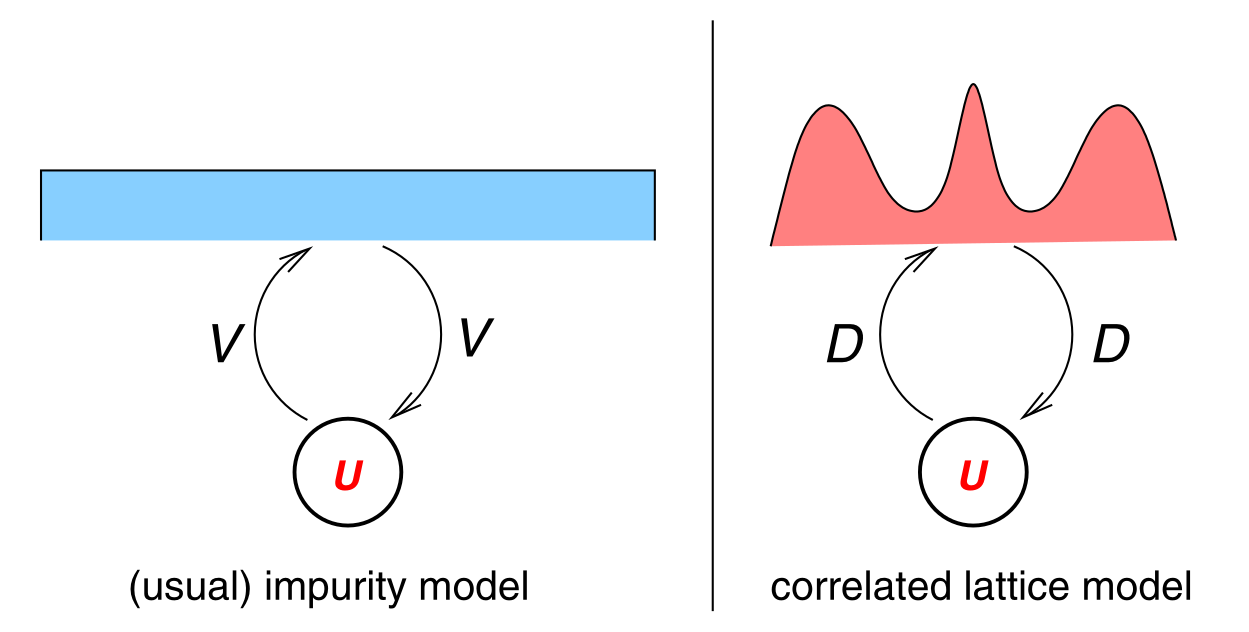
\includegraphics[width=0.5\textwidth]{../figures/correlated_bath.png}
\caption{"Comparison of the usual Anderson
impurity model of a strongly interacting site coupled via $V$ to
an uncorrelated featureless and wide conduction-electron band
(left-hand side) and the Hubbard model situation (right-hand
side). In the latter case, an electron leaving a correlated site
moves within the strongly correlated and narrow band of the
central peak. In this situation there is a kink at the effective
Kondo energy scale which is smaller than the width of the
narrow band." Image and caption source in footnote.}
\end{figure}


\section*{Hamiltonian}
We will include a local particle-hole symmetric correlation of strength \(U_b\) on the origin of the lattice:
\begin{equation}\begin{aligned}
	\mathcal{H} = \sum_{k\sigma}\epsilon_k \tau_{k\sigma} + \epsilon_d \left( \hat n_{d \uparrow} - \hat n_{d \downarrow} \right) ^2 + \sum_{k\sigma} \left(V_{k} c^\dagger_{k\sigma} c_{d\sigma} + h.c.\right) +J \vec{S_d}\cdot\vec{s} + K \vec{C_d}\cdot\vec{C}- U_b\left(\hat n_{0 \uparrow} - \hat n_{0 \downarrow}\right)^2 
\end{aligned}\end{equation}

\begin{figure}[htpb]
	\centering
	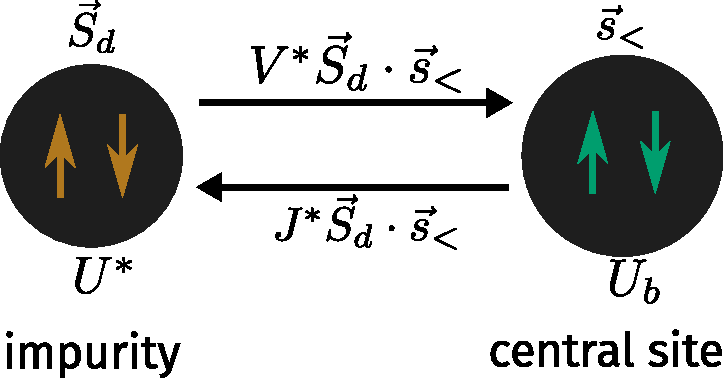
\includegraphics[width=0.5\textwidth]{../figures/zeromode.pdf}
	\caption{While we have studied the full model under renormalisation group, often we will turn to a simplified zero-bandwidth version of the model that is obtained by ignoring the kinetic energy part of the Hamiltonian. This zero-bandwidth model is effectively a two site model.}
\end{figure}

\section*{RG Equations}
The derivation of the RG equations are shown at the end. \(n_j\) is the number of \(k-\)states at the \(j^\text{th}\) isoenergetic shell. 
\begin{gather}
	\Delta U_b = 0, ~ ~\Delta U = 4V^2 n_j\left(\frac{1}{d_1} - \frac{1}{d_0}\right) - n_j\left(\frac{J^2}{d_2} - \frac{K^2}{d_3}\right),\\
	\Delta V = -\frac{3n_j V}{8}\left[\left(J + 4U_b/3\right) \left(\frac{1}{d_2} + \frac{1}{d_1}\right) + \left(K + 4U_b/3\right)\left(\frac{1}{d_3} + \frac{1}{d_0}\right)\right],\\
	\Delta J = -\frac{n_j J\left(J + 4U_b\right)}{d_2},~ ~\Delta K = -\frac{n_j K\left(K + 4U_b\right)}{d_3}
\end{gather}

The denominators are
\begin{equation}\begin{aligned}
	d_0 = \omega - \frac{D}{2} + \frac{U_b}{2} - \frac{U}{2} + \frac{K}{4}, \quad d_1 = \omega - \frac{D}{2} + \frac{U_b}{2} + \frac{U}{2} + \frac{J}{4}, \quad d_2 = \omega - \frac{D}{2} + \frac{U_b}{2} + \frac{J}{4}, \quad d_3 = \omega - \frac{D}{2} + \frac{U_b}{2} + \frac{K}{4}
\end{aligned}\end{equation}

\paragraph{Important points regarding notation}
\begin{itemize}
	\item The labels \(U_0,J_0,V_0\) that may occur in the axes of the plots or anywhere else represent the bare values of the couplings \(U,J\) and \(V\). 
	\item Throughout the results, the bare value of \(U_b\) is set to the negative of the bare value of \(U_0\): \(U_b = -U_0\). This means that whenever we vary \(U_0\) along the axis of a plot, we are simultaneous varying \(U_b\).	
\end{itemize}

\section*{Phase diagram}

\begin{center}
	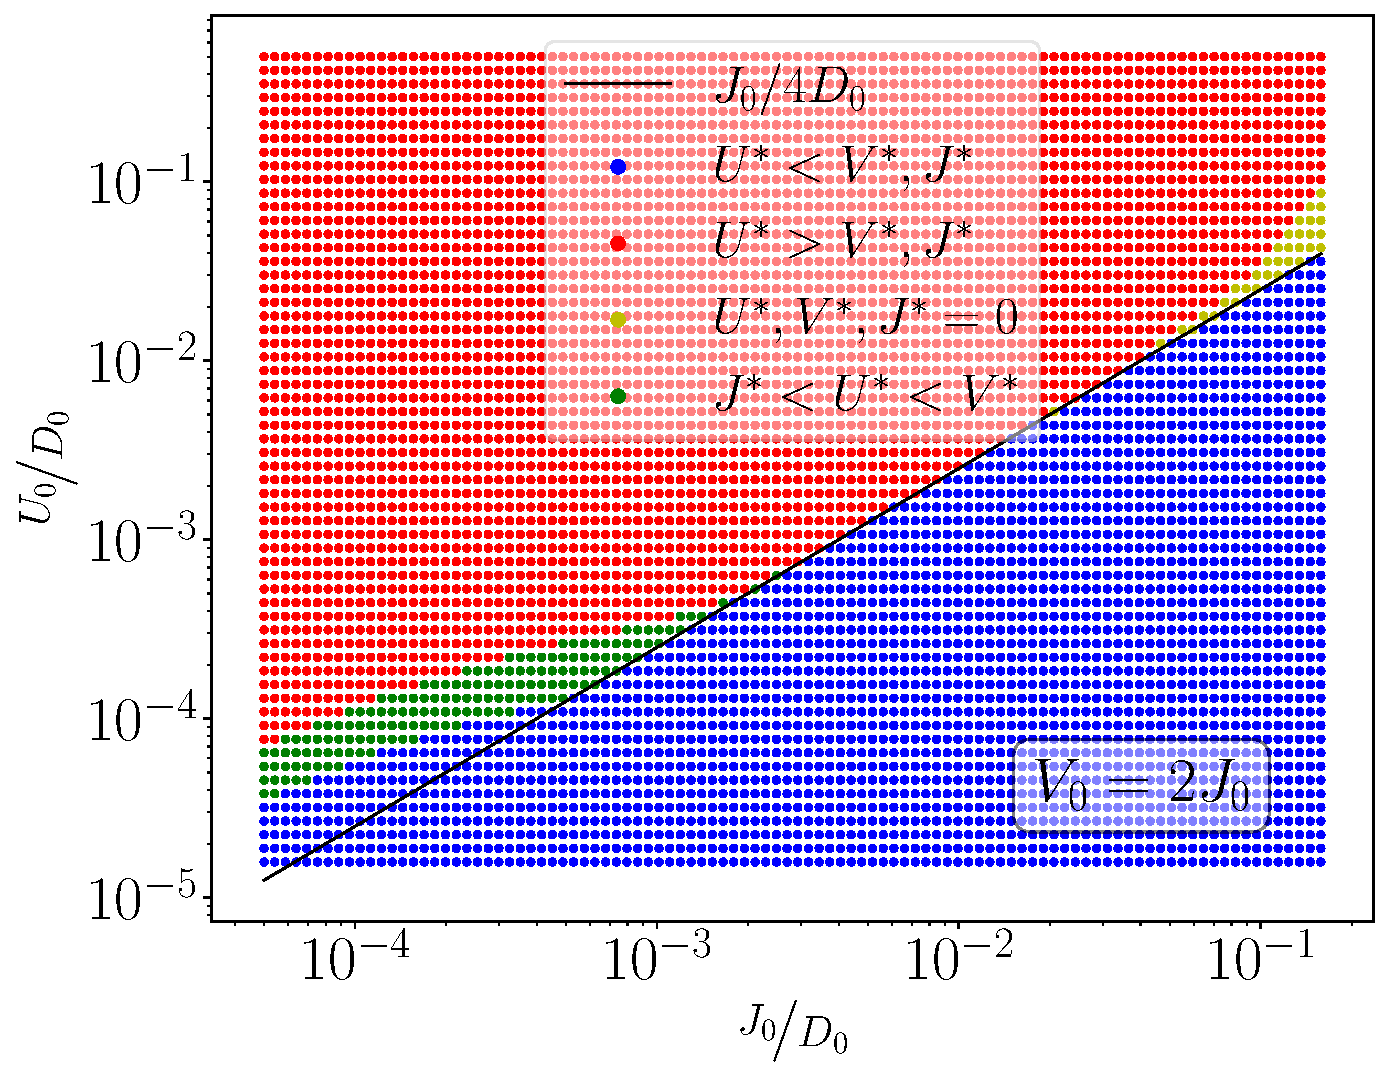
\includegraphics[width=0.9\textwidth]{../figures/phase-map_D=1000.pdf}
\end{center}

\begin{center}
\begin{tabular}{|c|c|c|c|c|}
\hline
phase & RG flow & fixed point & GS & 2-site GS \\ 
\hline
blue & \(\Delta U <0, \Delta J,\Delta V>0\) & \(U^* \ll V^* \ll J^*\) & SS & \(\ket{SS}=\ket{\uparrow,\downarrow} - \ket{\downarrow, \uparrow}\)  \\ 
green &  \(\Delta U < 0, \Delta J < 0,\Delta V>0\) & \(V^* < U^* \ll V^*\) & SS + CT-0 & \(c\ket{SS} + \sqrt{1-c^2}\ket{CT-0}\)  \\  
red &  \(\Delta U > 0, \Delta J,\Delta V<0\) & \(U^* \gg 1,  V^* = J^* = 0\) & decoupled LM & \(\left\{\ket{\uparrow}, \ket{\downarrow} \right\} \otimes \left\{\ket{0}, \ket{2}\right\} \) \\
yellow &  \(\Delta U, \Delta J,\Delta V < 0\) & \(U^* = V^* = J^* = 0\) & lattice & \(\left\{\ket{\uparrow}, \ket{\downarrow}, \ket{0}, \ket{2} \right\} \otimes \left\{\ket{0}, \ket{2}\right\}\) \\
\hline
\end{tabular}
\end{center}



\section*{Overlap of ground state against spin singlet and charge triplet zero states}
\begin{center}
	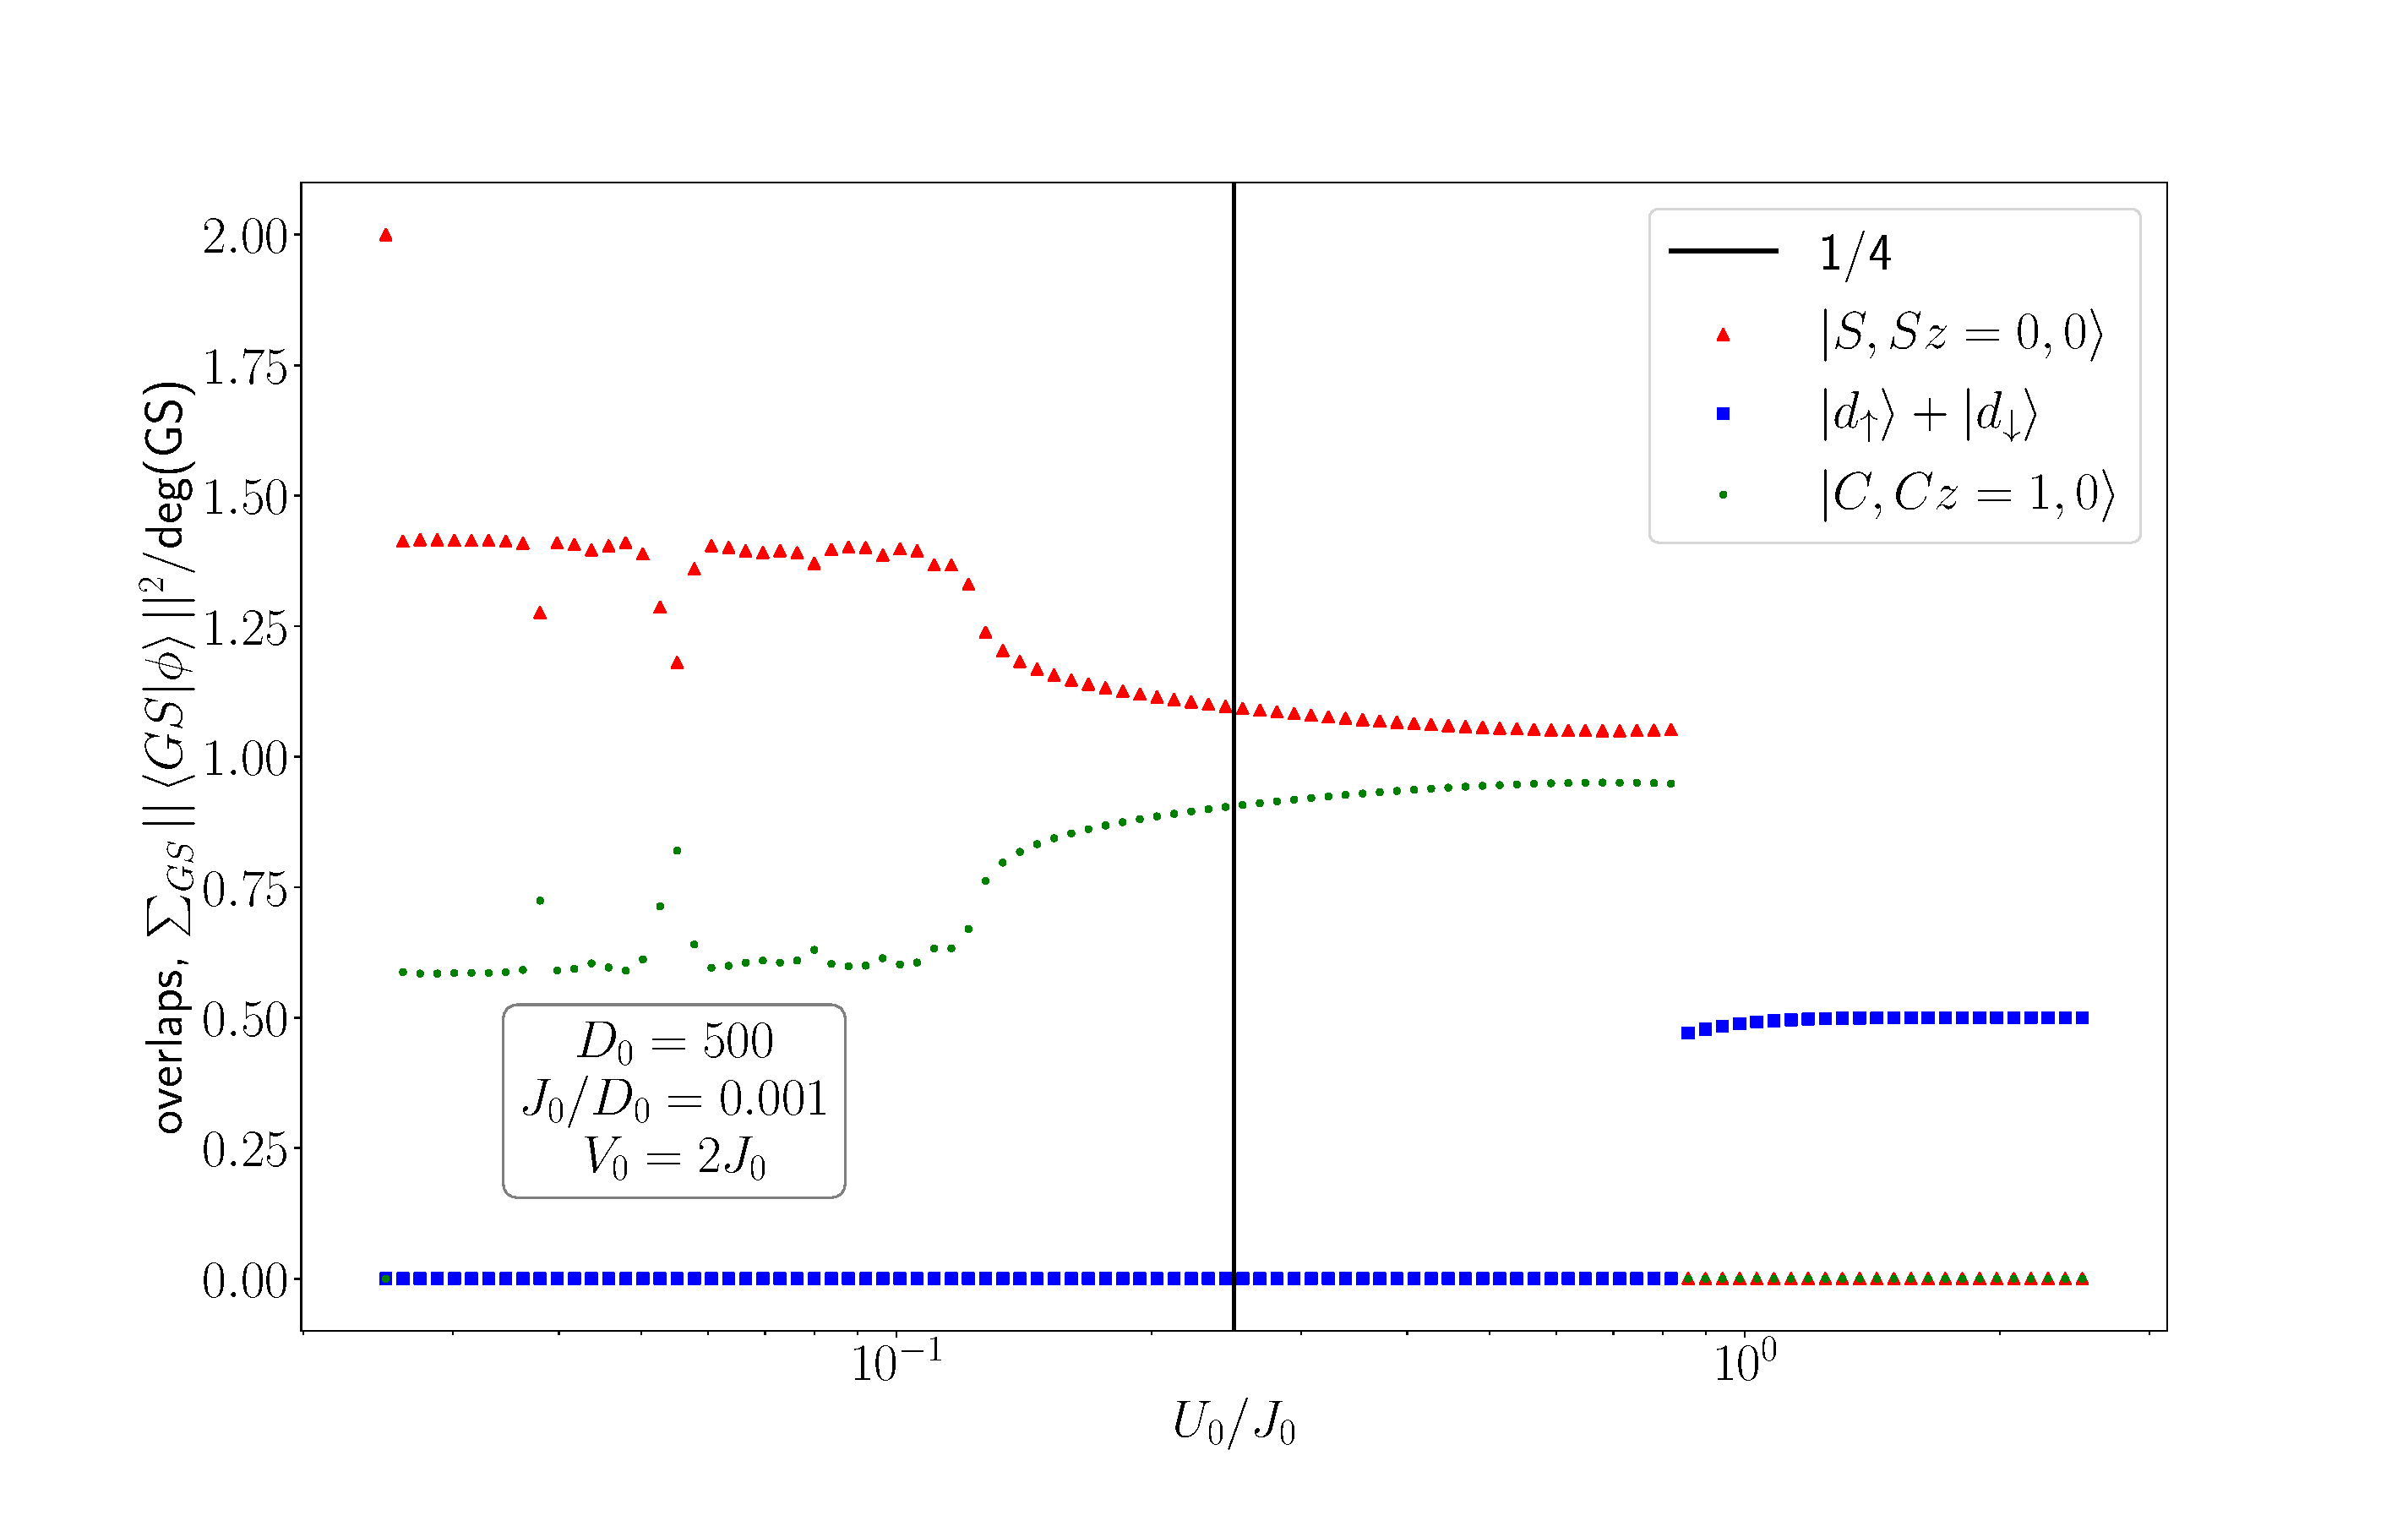
\includegraphics[width=0.8\textwidth]{../figures/overlaps_gs_D=500,J=0.500.pdf}\\
	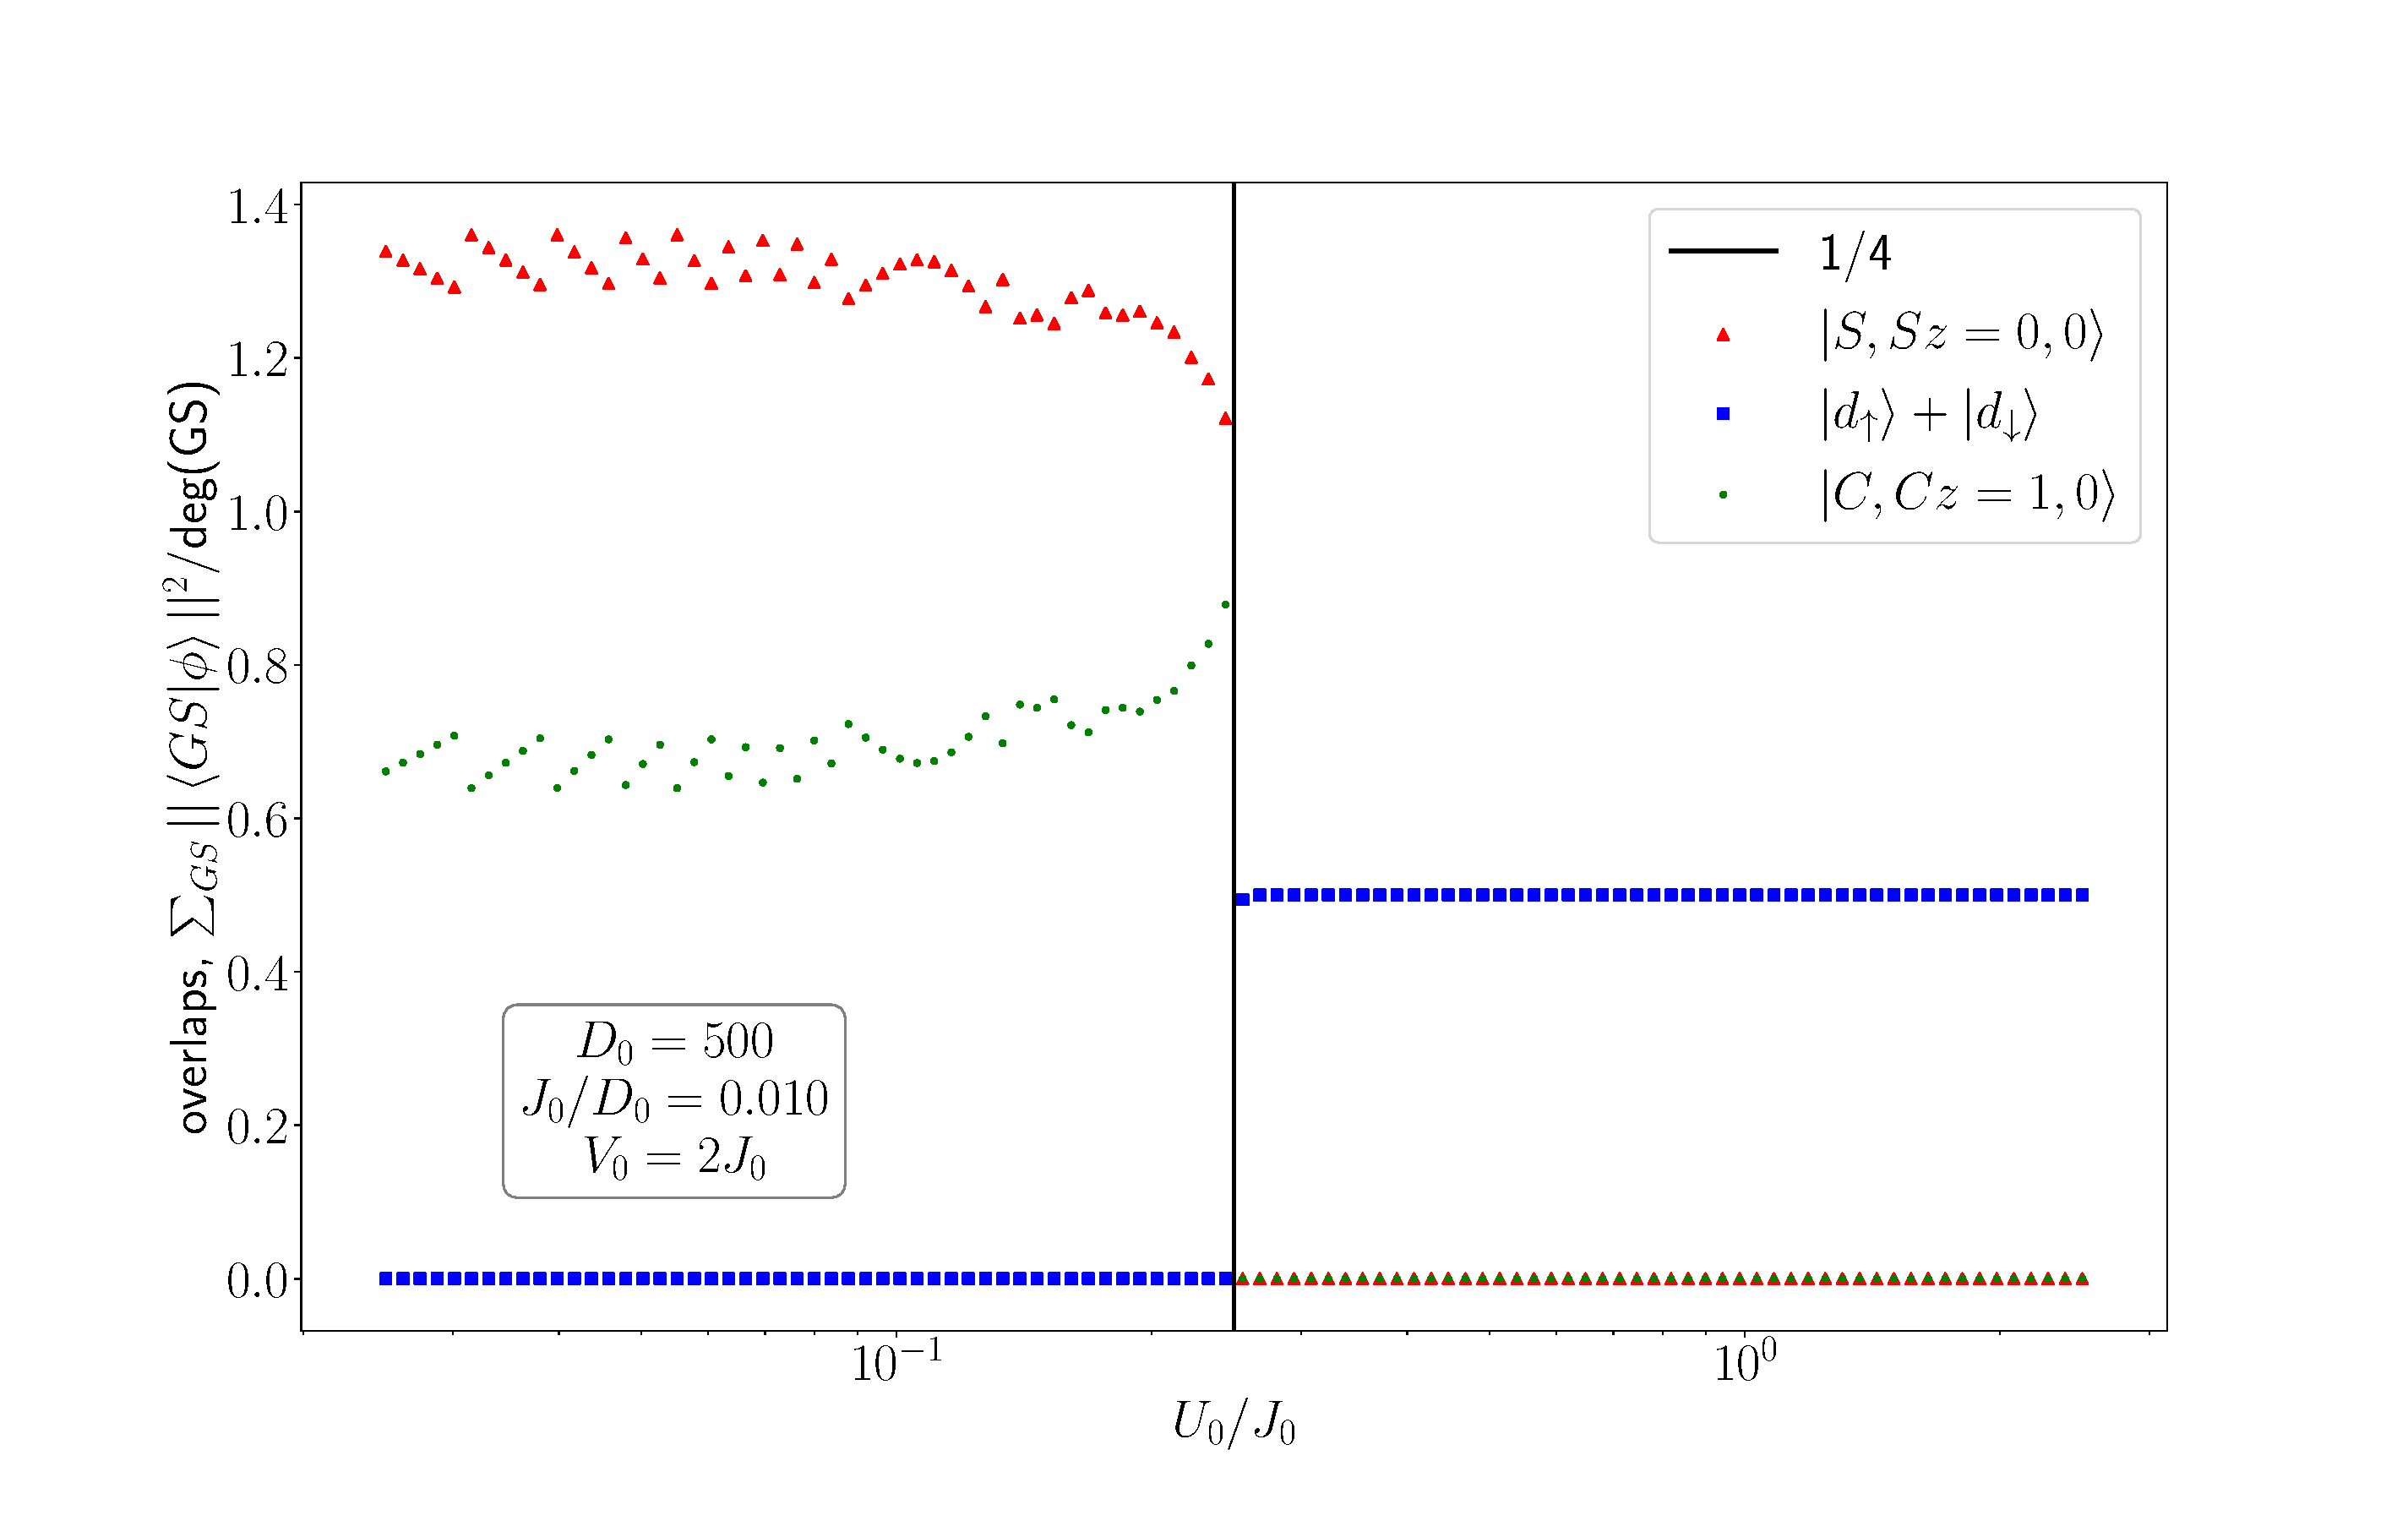
\includegraphics[width=0.8\textwidth]{../figures/overlaps_gs_D=500,J=5.000.pdf}\\
	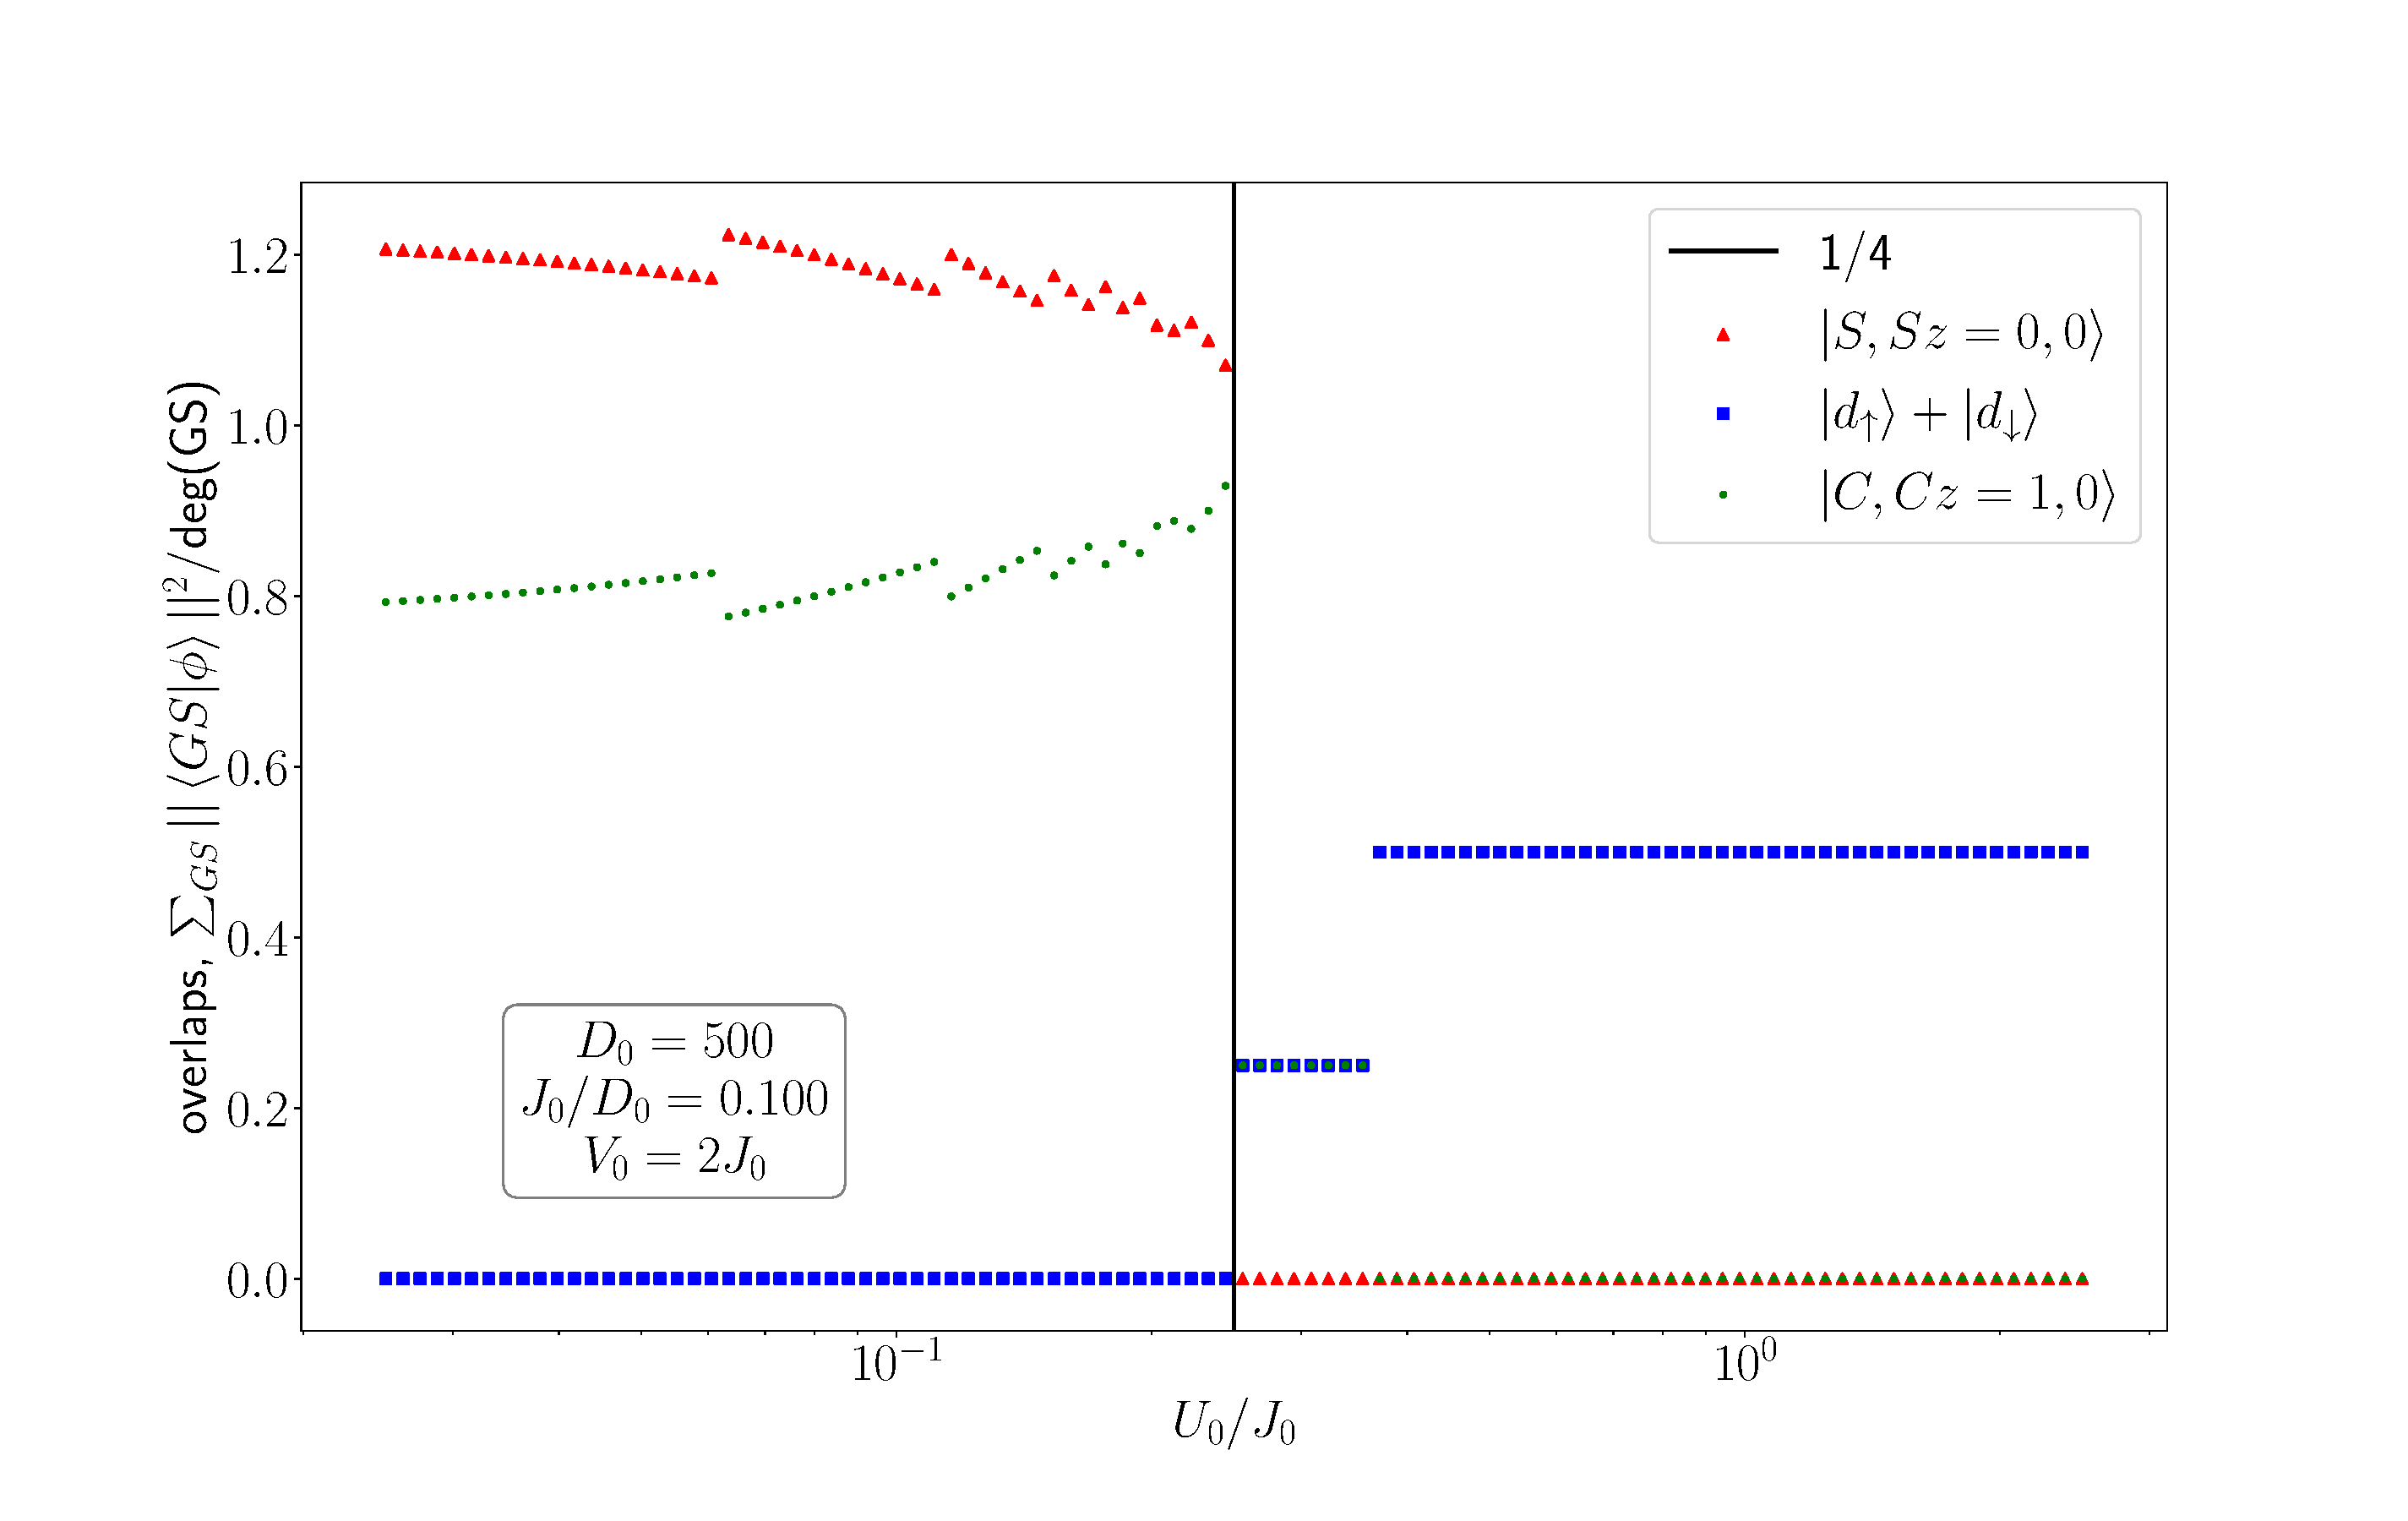
\includegraphics[width=0.8\textwidth]{../figures/overlaps_gs_D=500,J=50.000.pdf}
\end{center}

\section*{Spin and charge correlations in ground state}
\begin{center}
	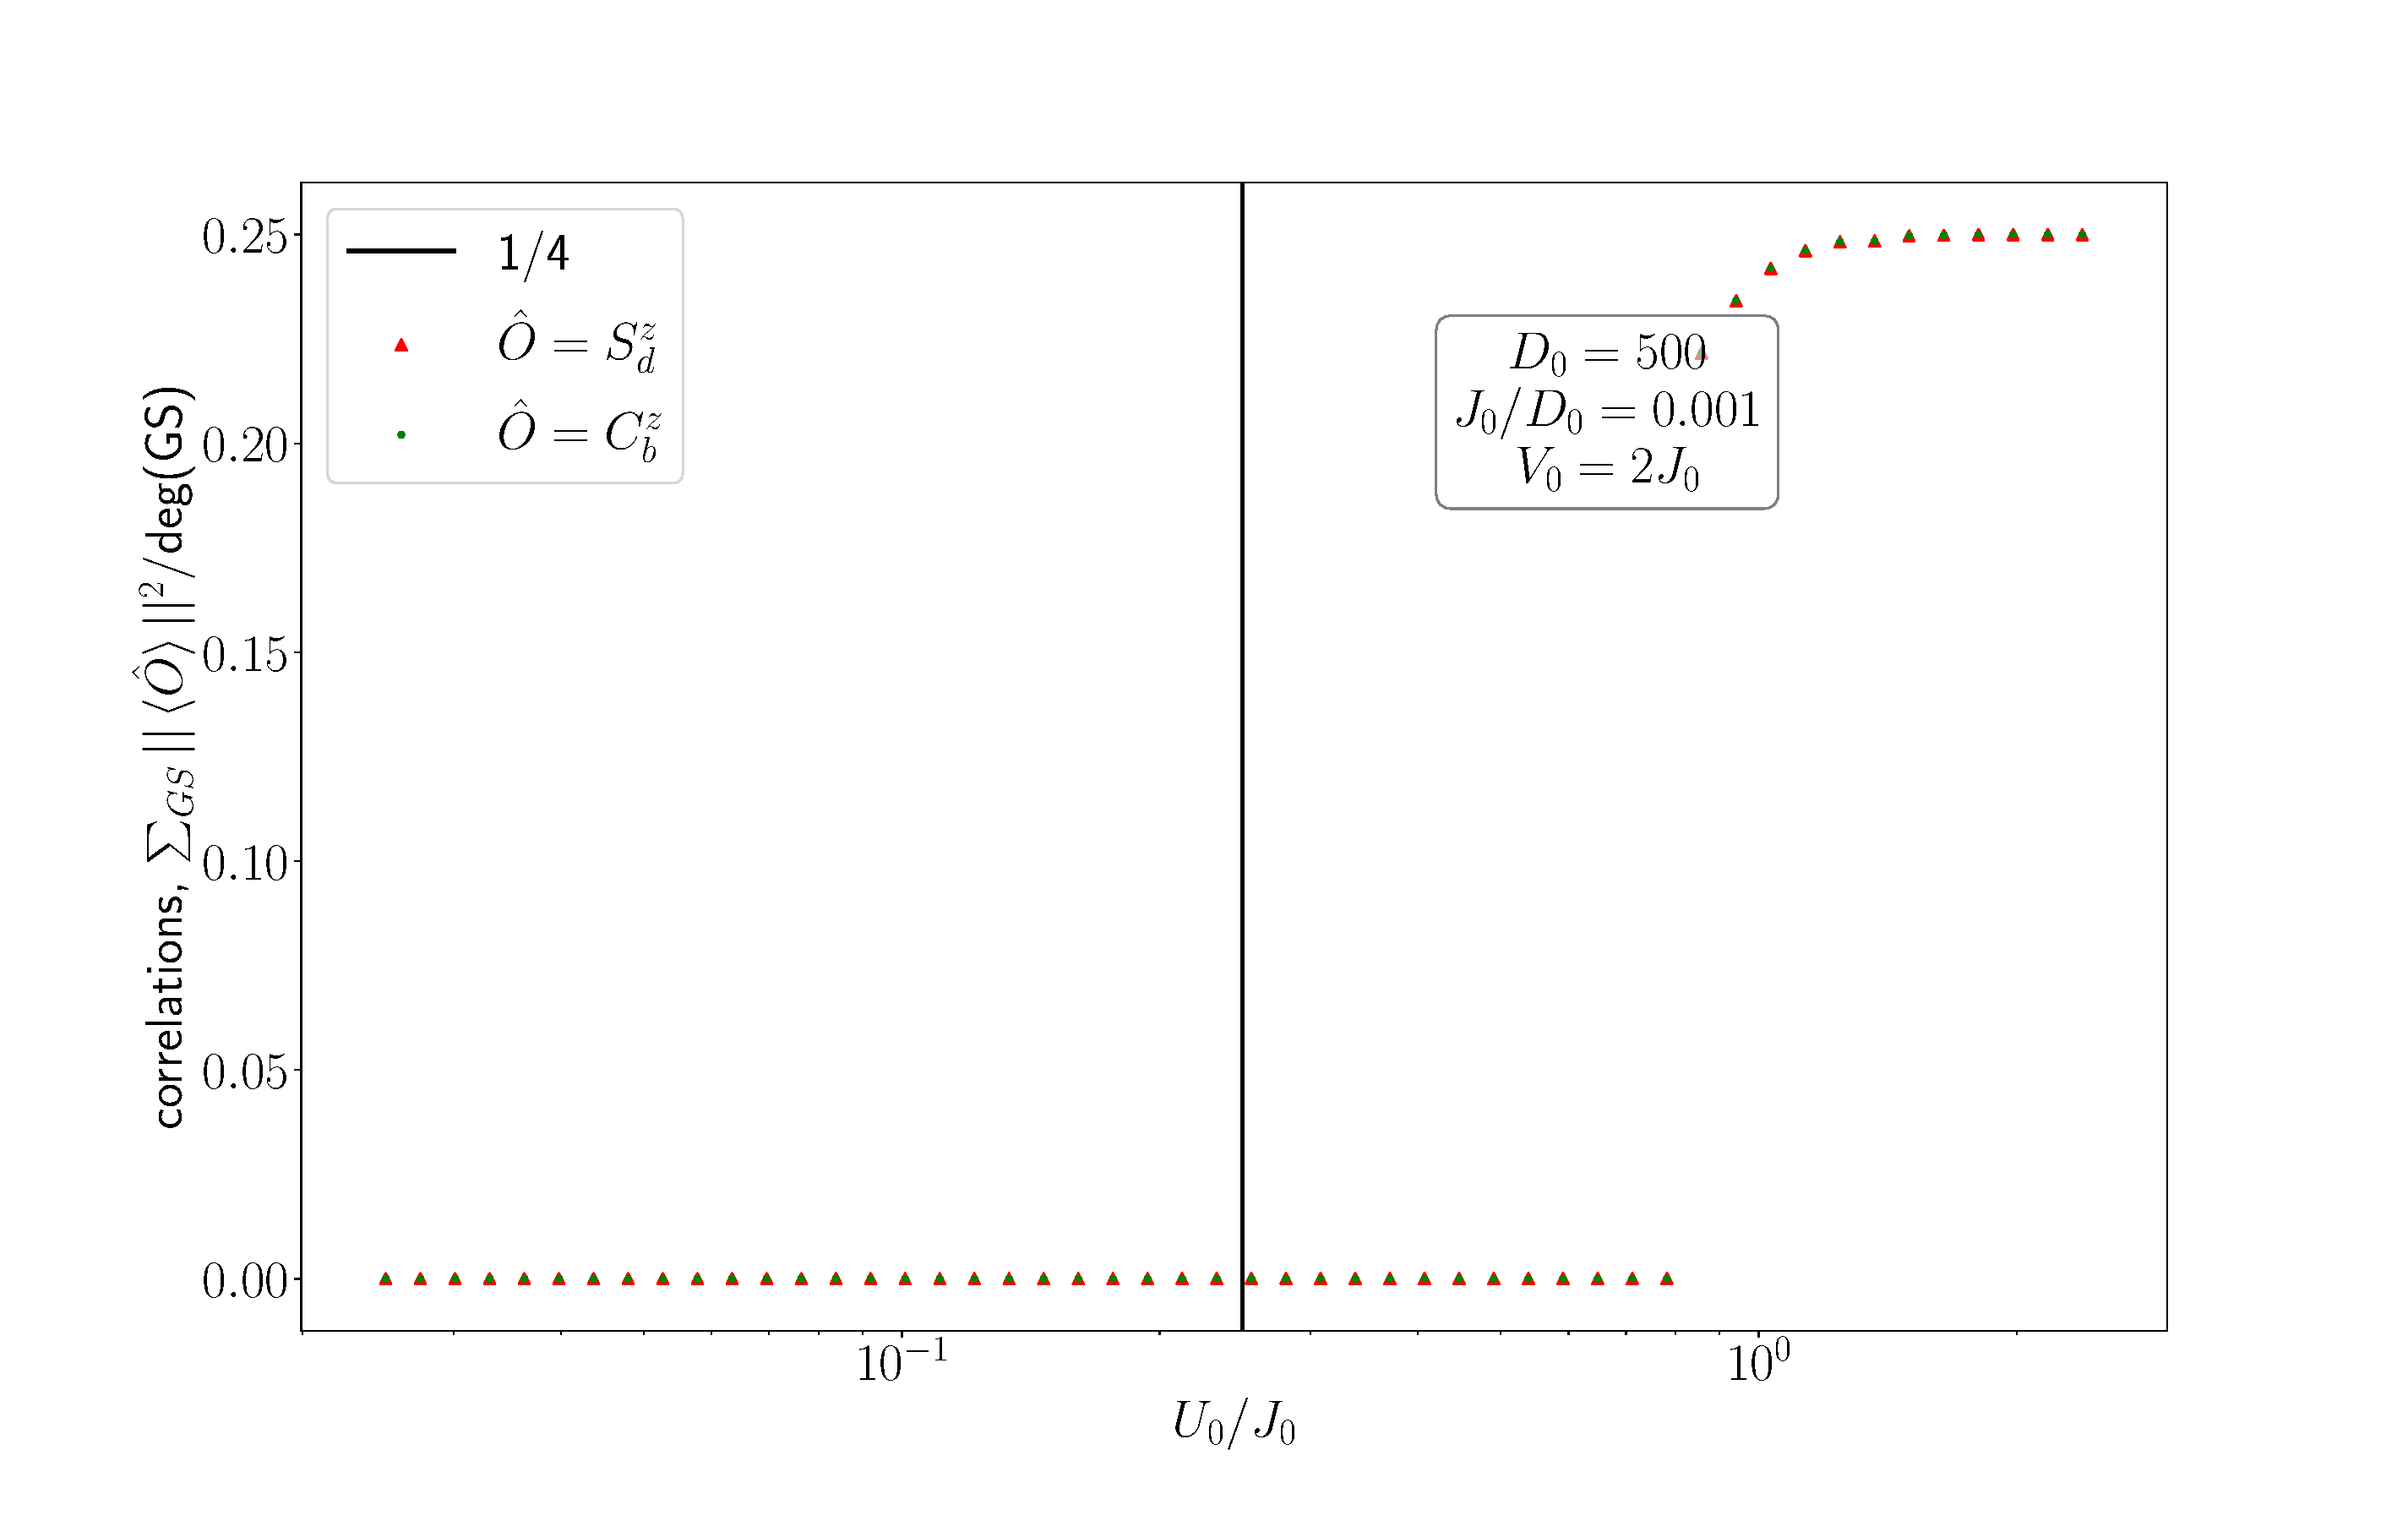
\includegraphics[width=0.8\textwidth]{../figures/corrs_gs_D=500,J=0.500.pdf}\\
	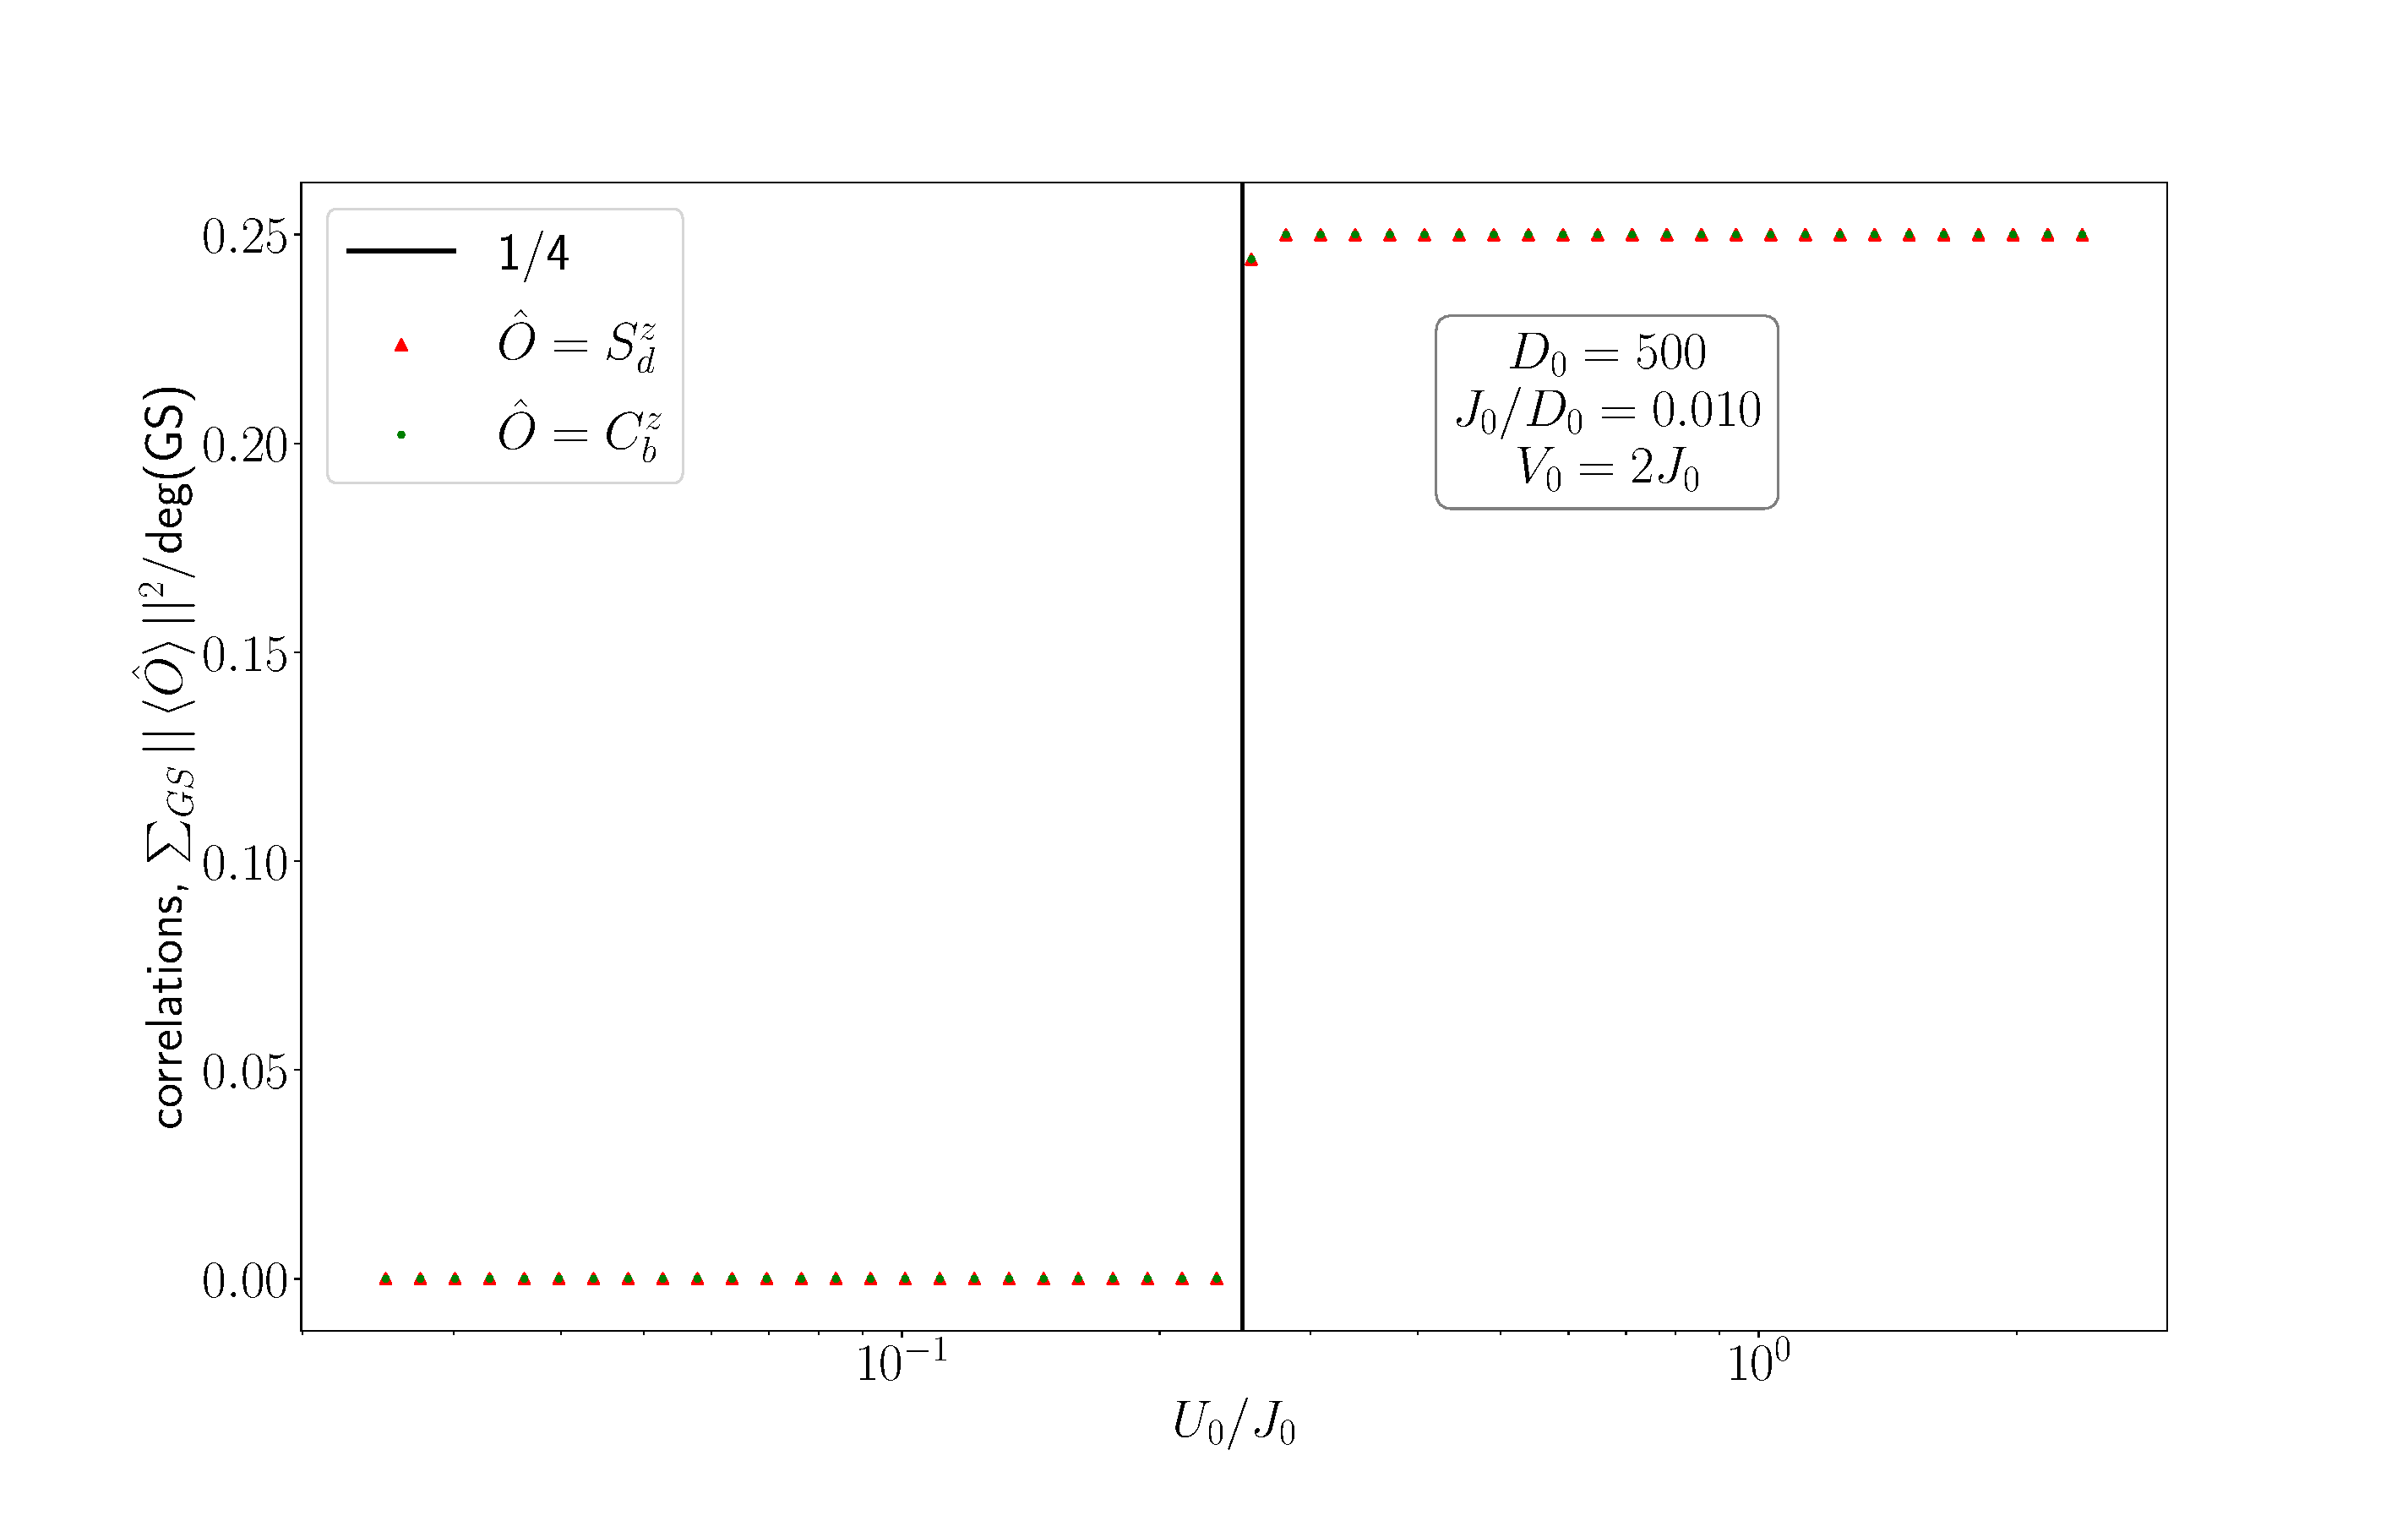
\includegraphics[width=0.8\textwidth]{../figures/corrs_gs_D=500,J=5.000.pdf}\\
	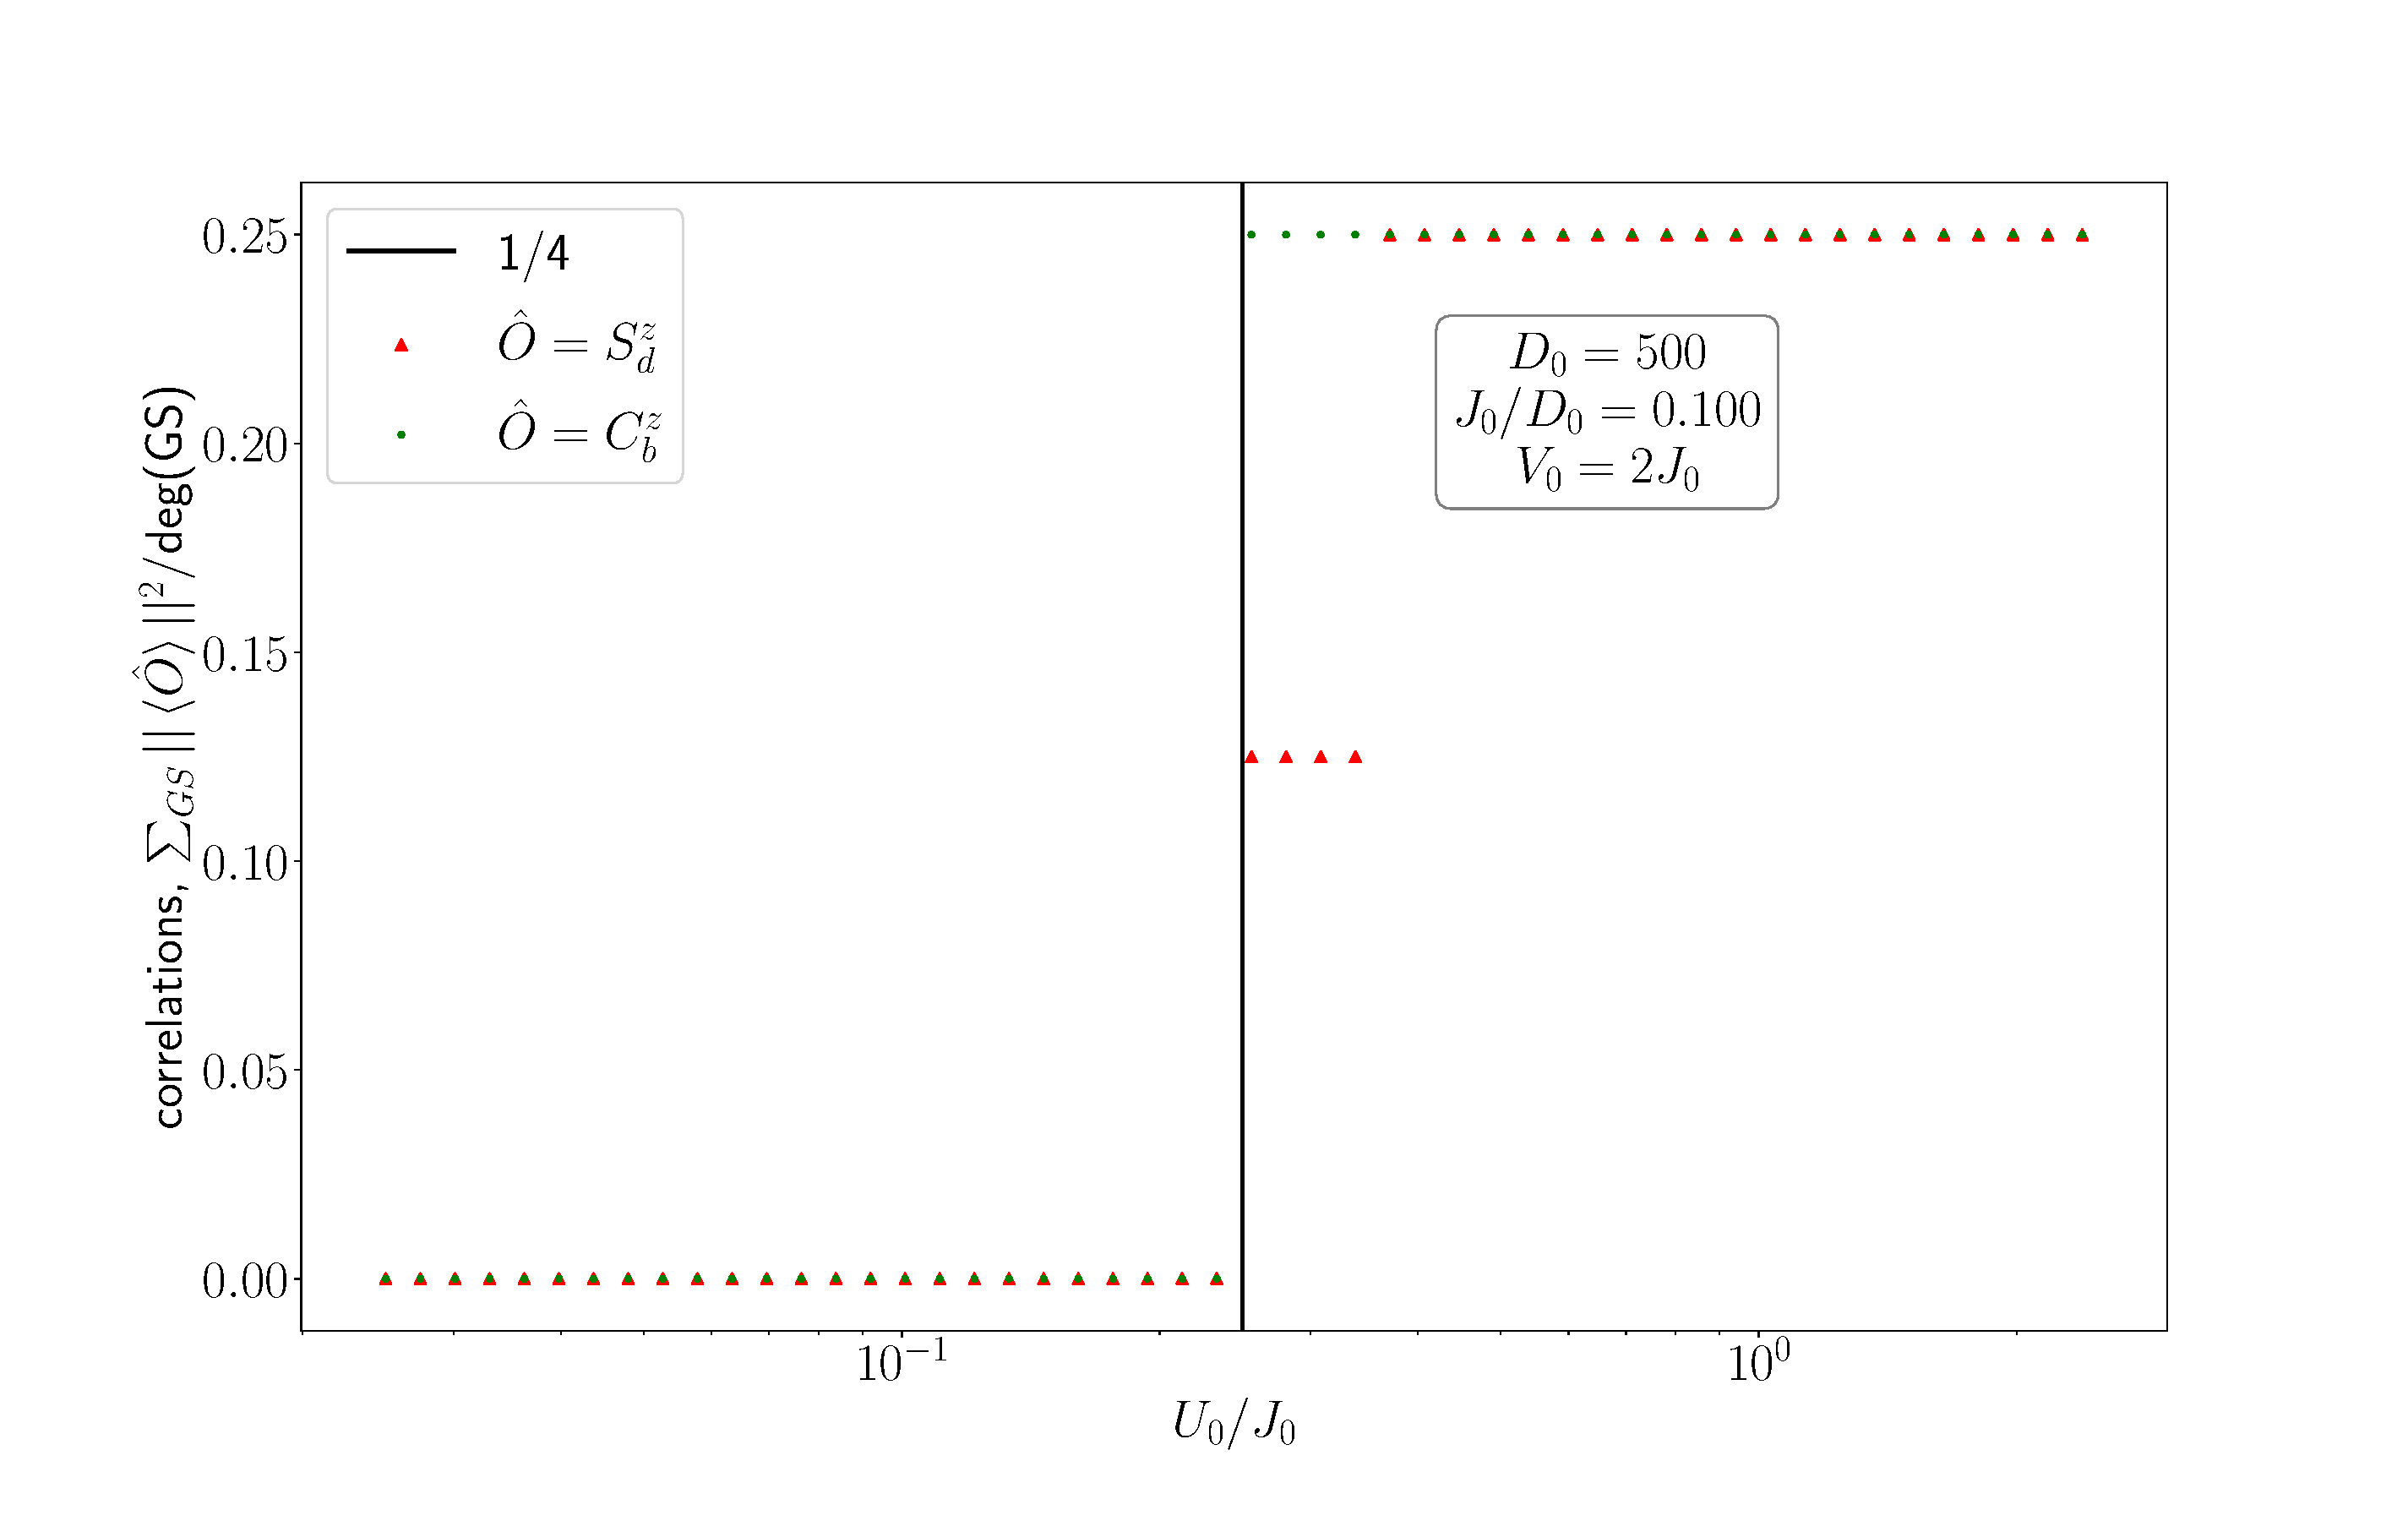
\includegraphics[width=0.8\textwidth]{../figures/corrs_gs_D=500,J=50.000.pdf}
\end{center}

\section*{\large Behaviour of \(\mathcal{F}\), the gap and the small parameter}
These quantities are related to the local Fermi liquid of the Kondo strong-coupling fixed point and the perturbation theory associated with it. \(min(\delta E)\) is the gap in the spectrum of the two-site Hamiltonian; this which acts as the denominator for the perturbation theoretic calculations. \(t^2/\delta E\) is the small parameter for the expansion, \(t\) being the tight-binding hopping. \(\mathcal{F}\) is the strength of the local Fermi liquid \((\mathcal{F} \hat n_{1 \uparrow} \hat n_{1 \downarrow})\).
\begin{center}
	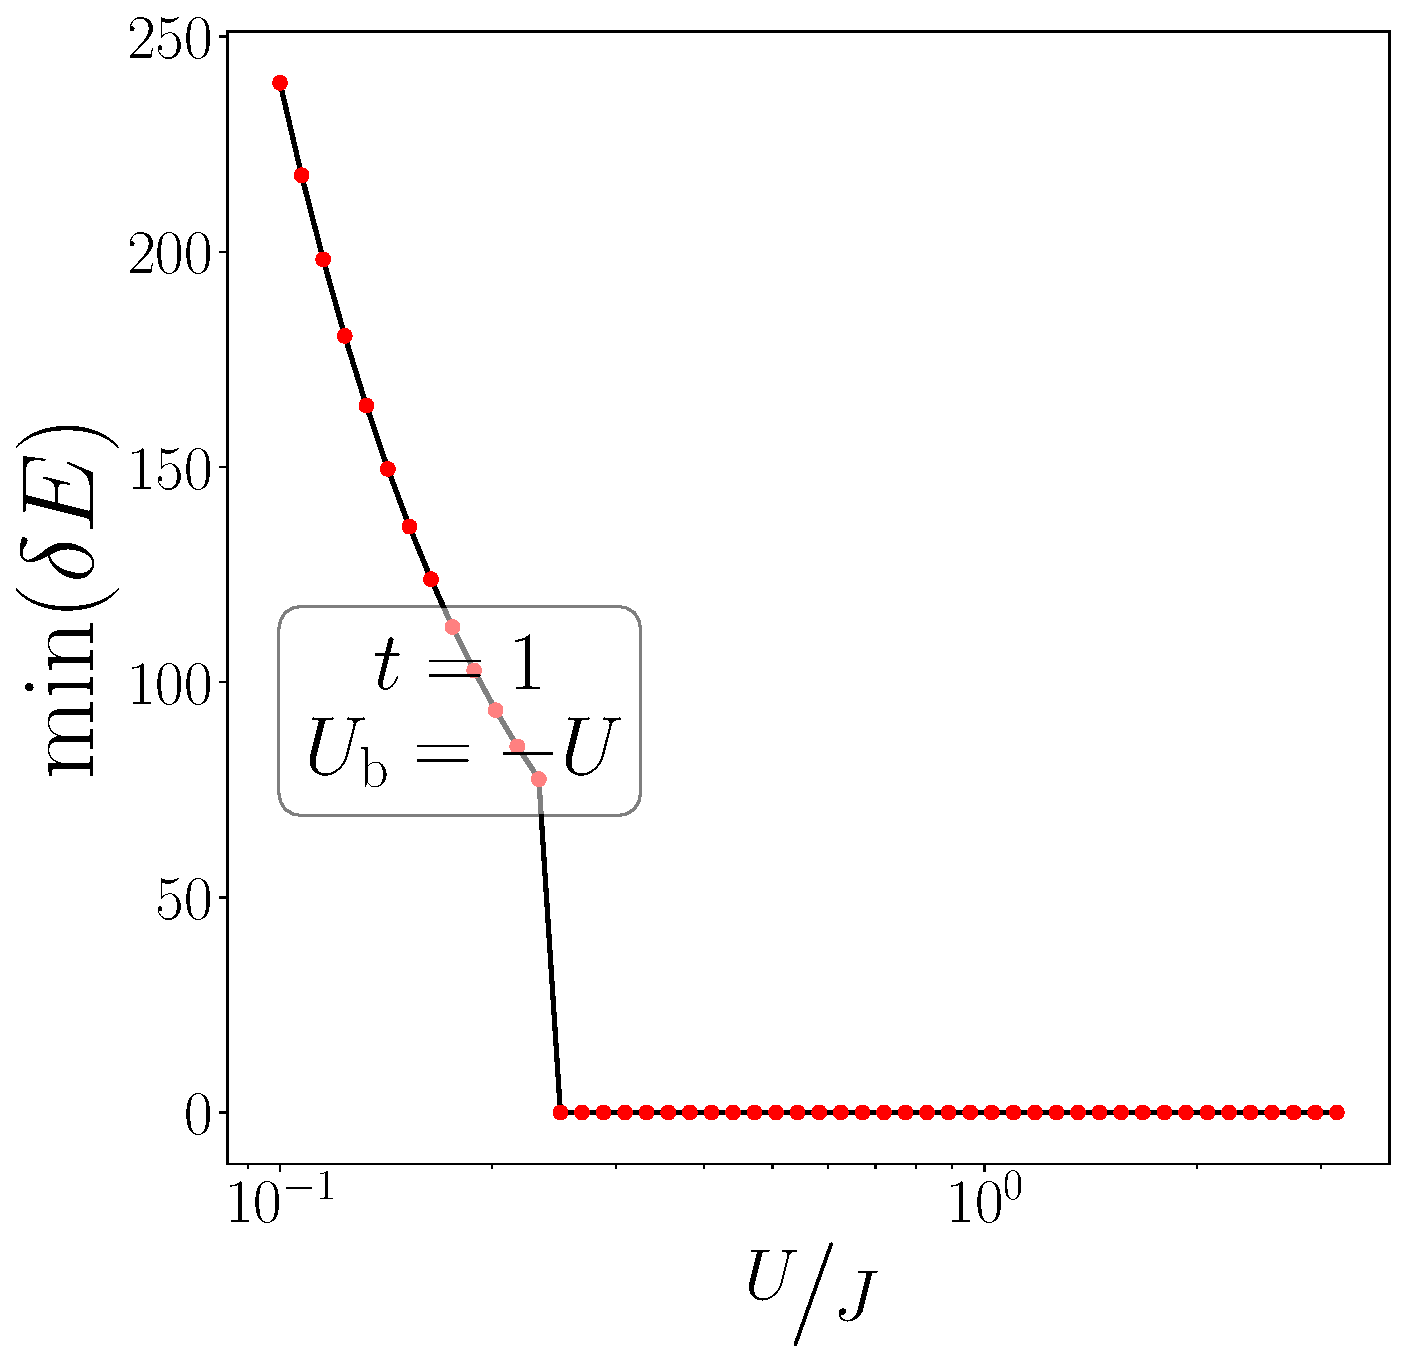
\includegraphics[width=0.32\textwidth]{../figures/gap-t=1.000,J=100,V=2J,Ubath=-U,N=4,U=0.100,3.162,50.pdf}
	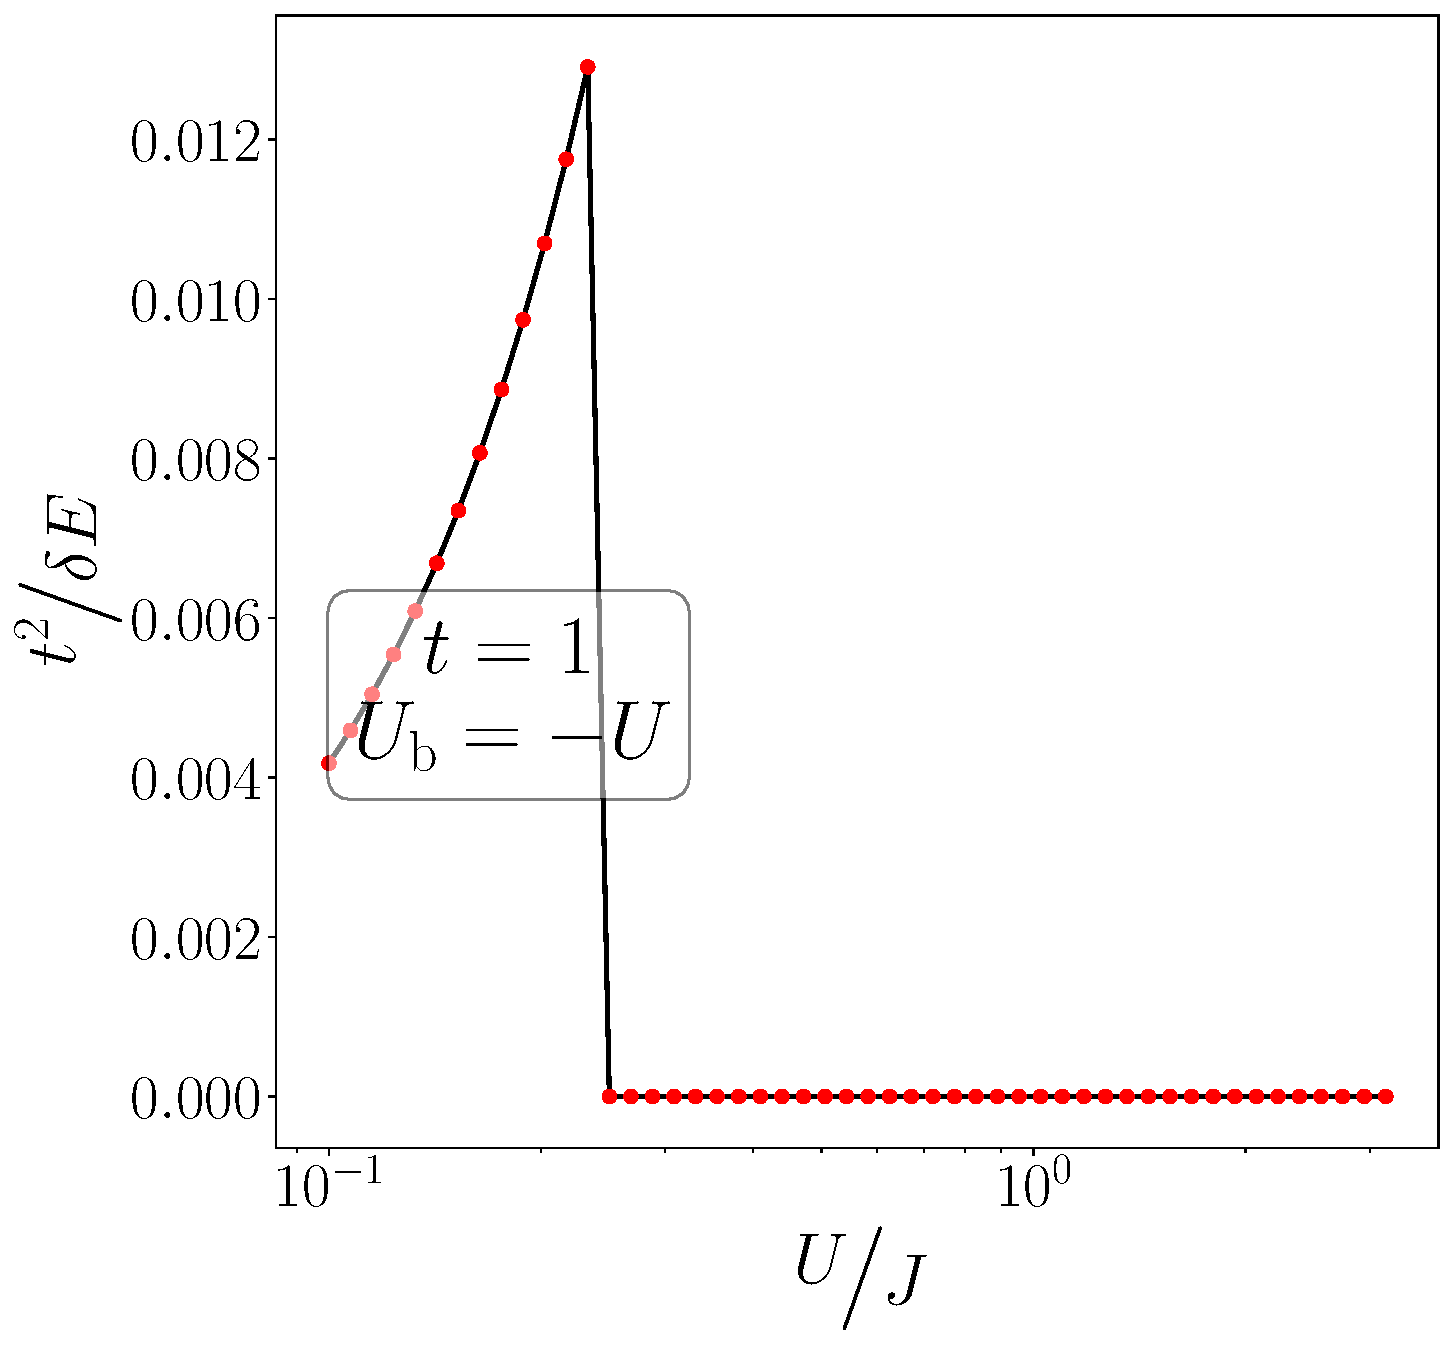
\includegraphics[width=0.32\textwidth]{../figures/par-t=1.000,J=100,V=2J,Ubath=-U,N=4,U=0.100,3.162,50.pdf}
	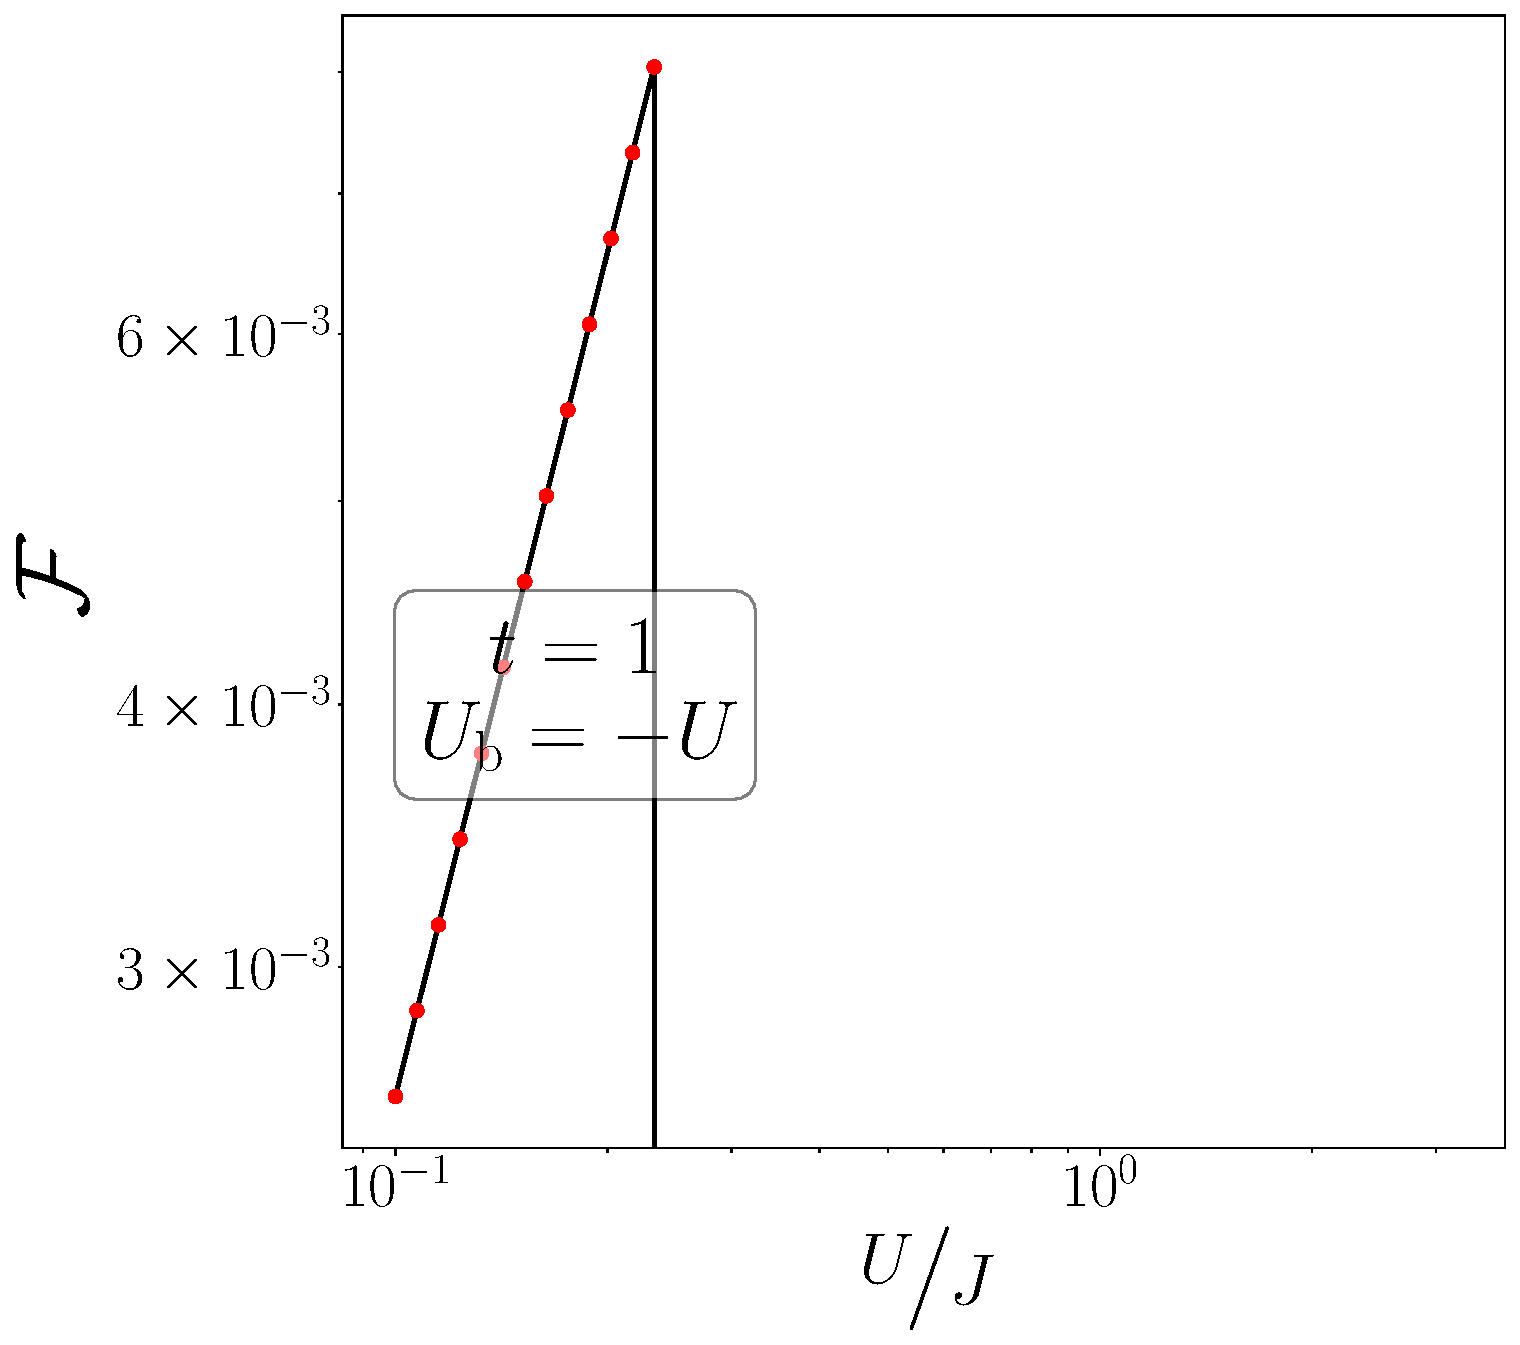
\includegraphics[width=0.32\textwidth]{../figures/lfl-t=1.000,J=100,V=2J,Ubath=-U,N=4,U=0.100,3.162,50.pdf}
\end{center}

\section*{\large Behaviour of correlation within the Kondo cloud}
\begin{center}
	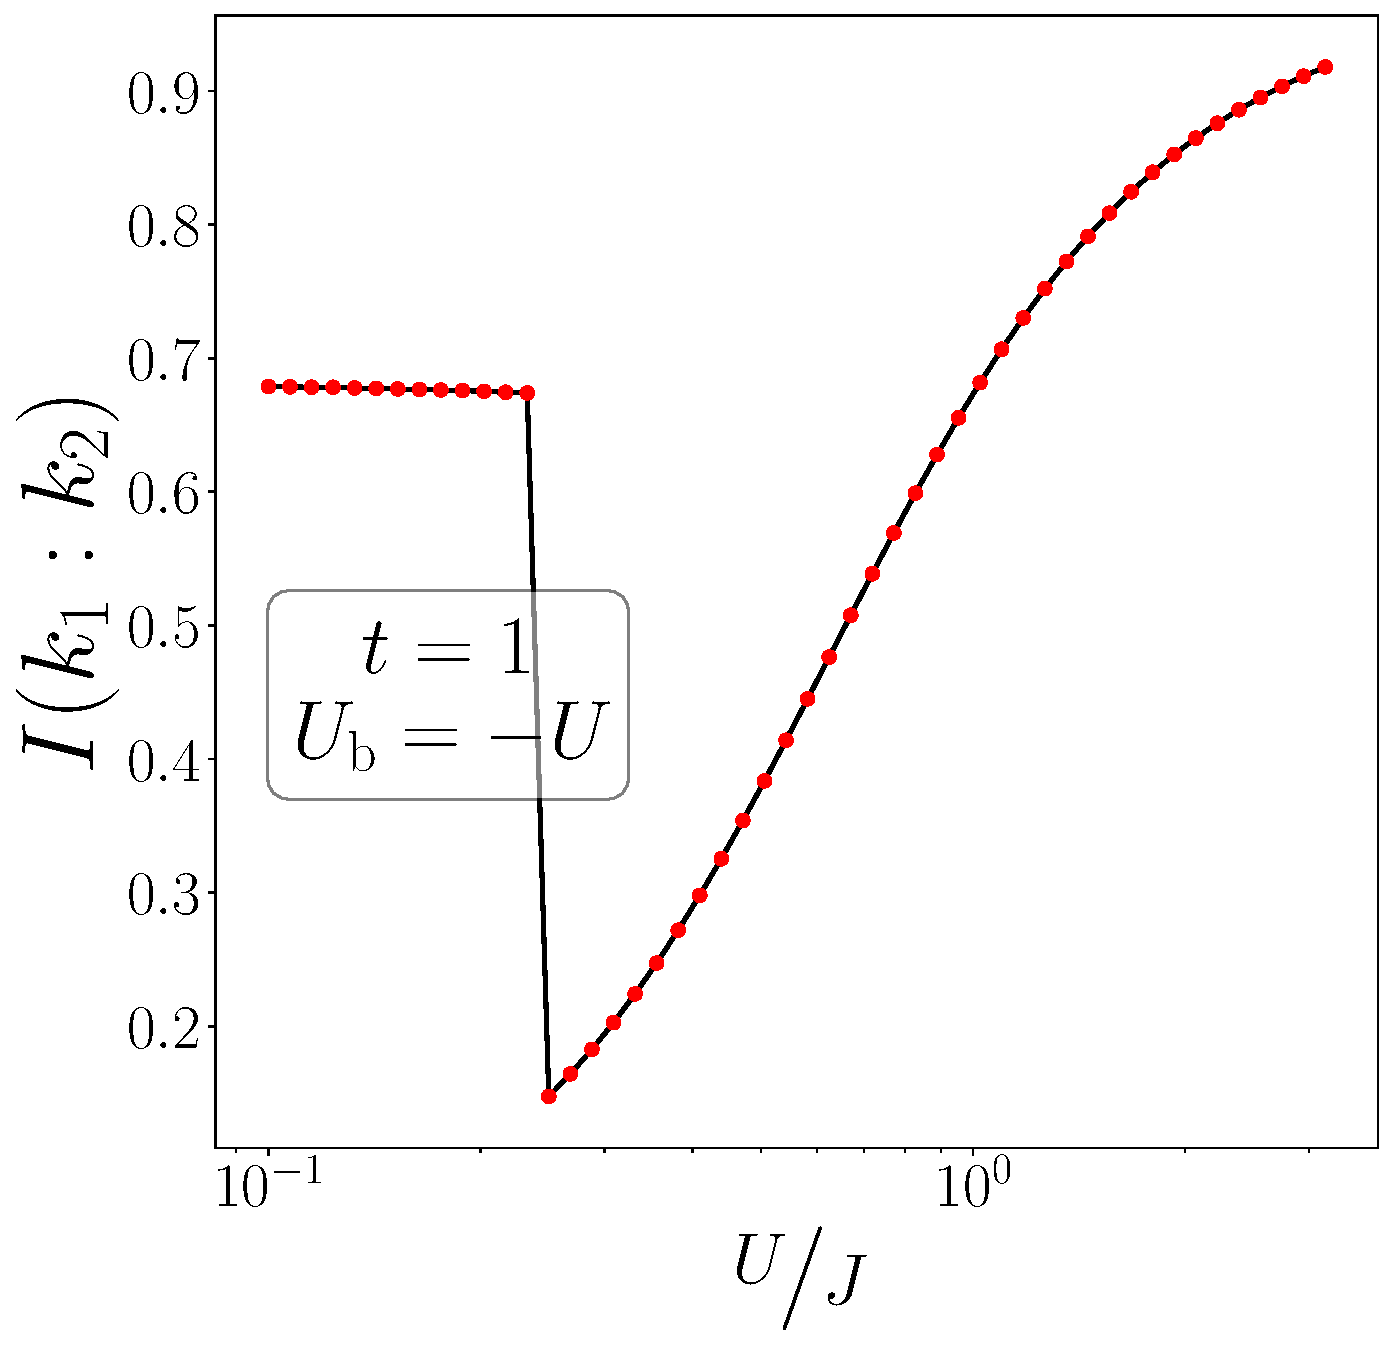
\includegraphics[width=0.24\textwidth]{../figures/corr-k-t=1.000,J=100,V=2J,Ubath=-U,N=4,U=0.100,3.162,50.pdf}
	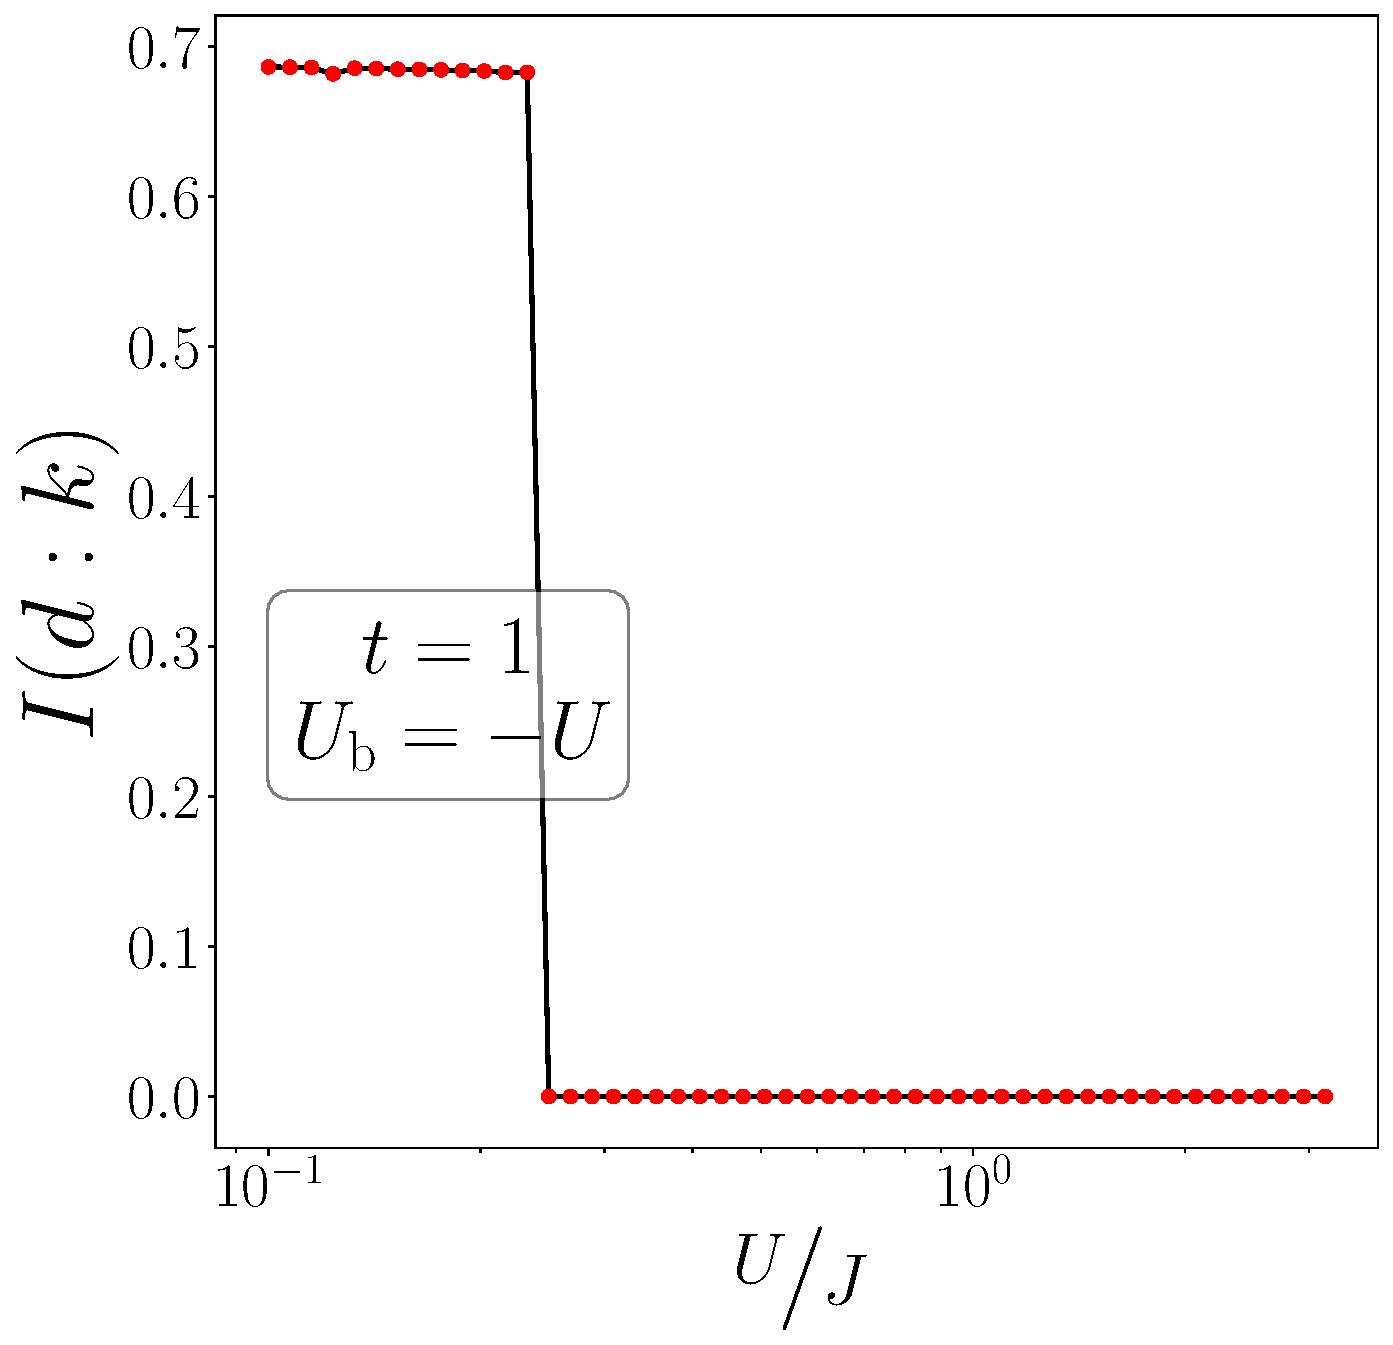
\includegraphics[width=0.24\textwidth]{../figures/mi-dk-t=1.000,J=100,V=2J,Ubath=-U,N=4,U=0.100,3.162,50.pdf}
	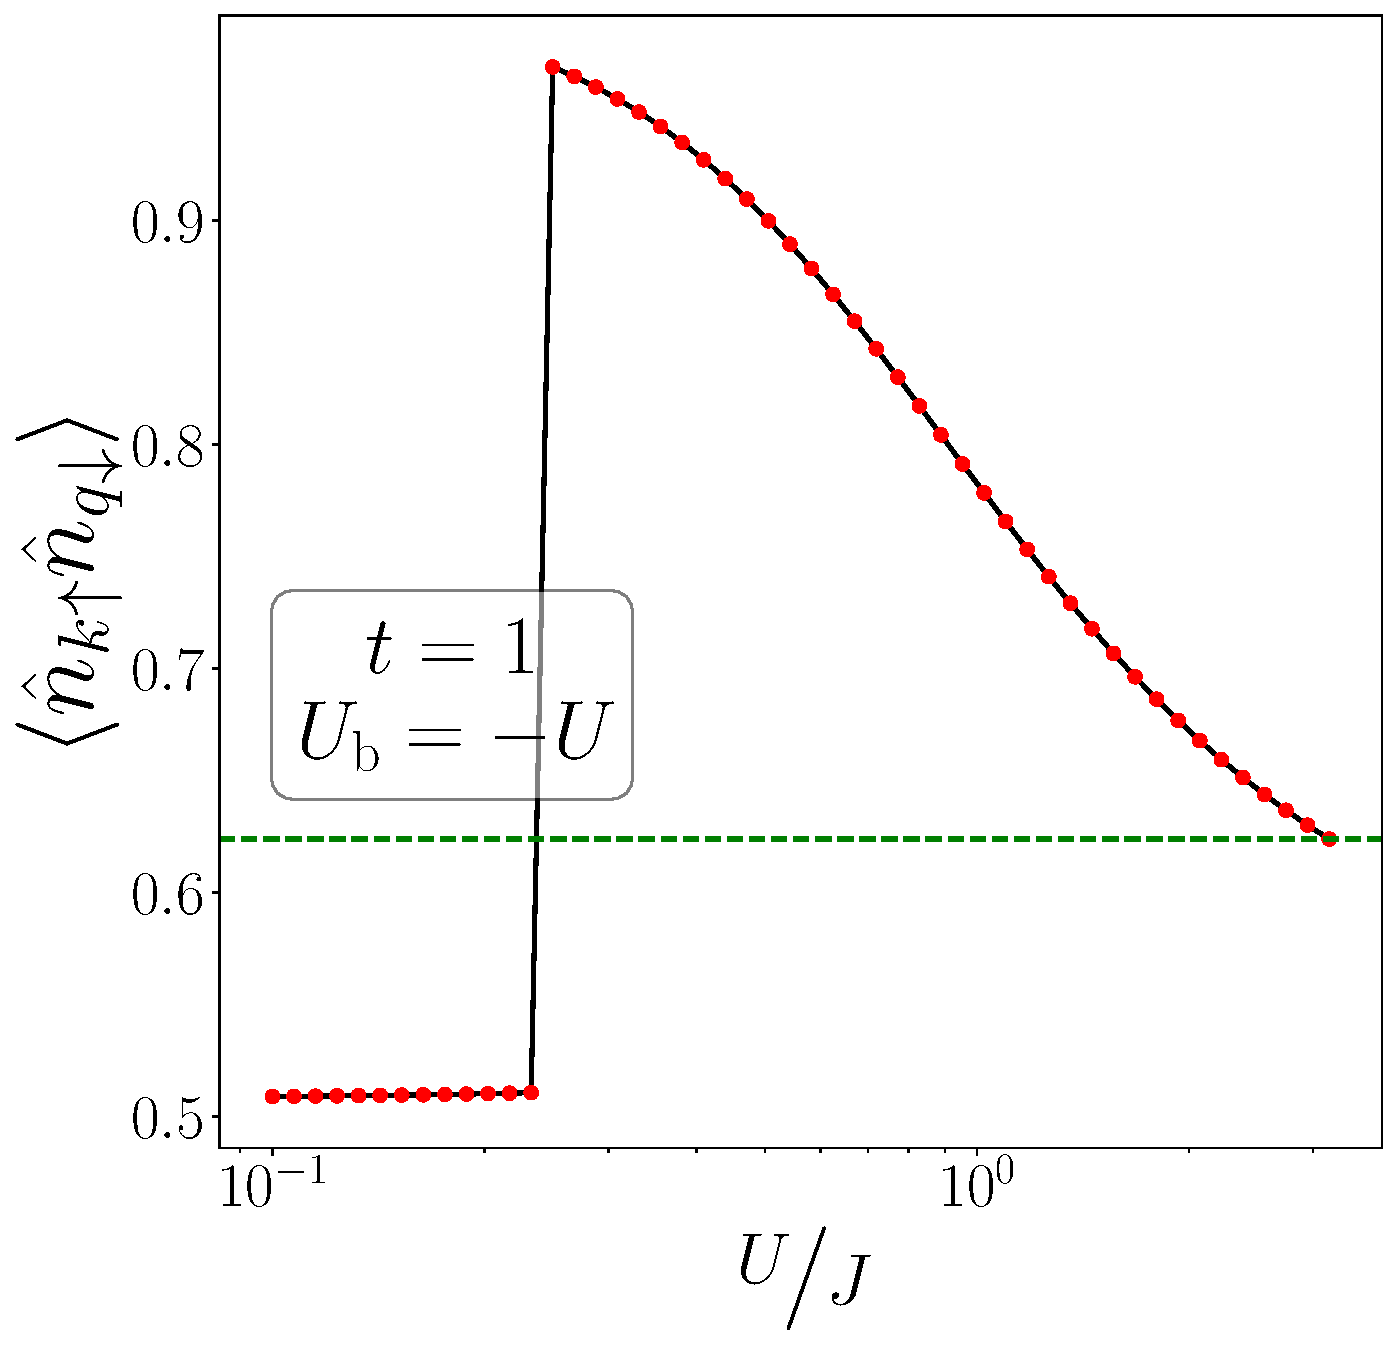
\includegraphics[width=0.24\textwidth]{../figures/corr-k-diag-t=1.000,J=100,V=2J,Ubath=-U,N=4,U=0.100,3.162,50.pdf}
	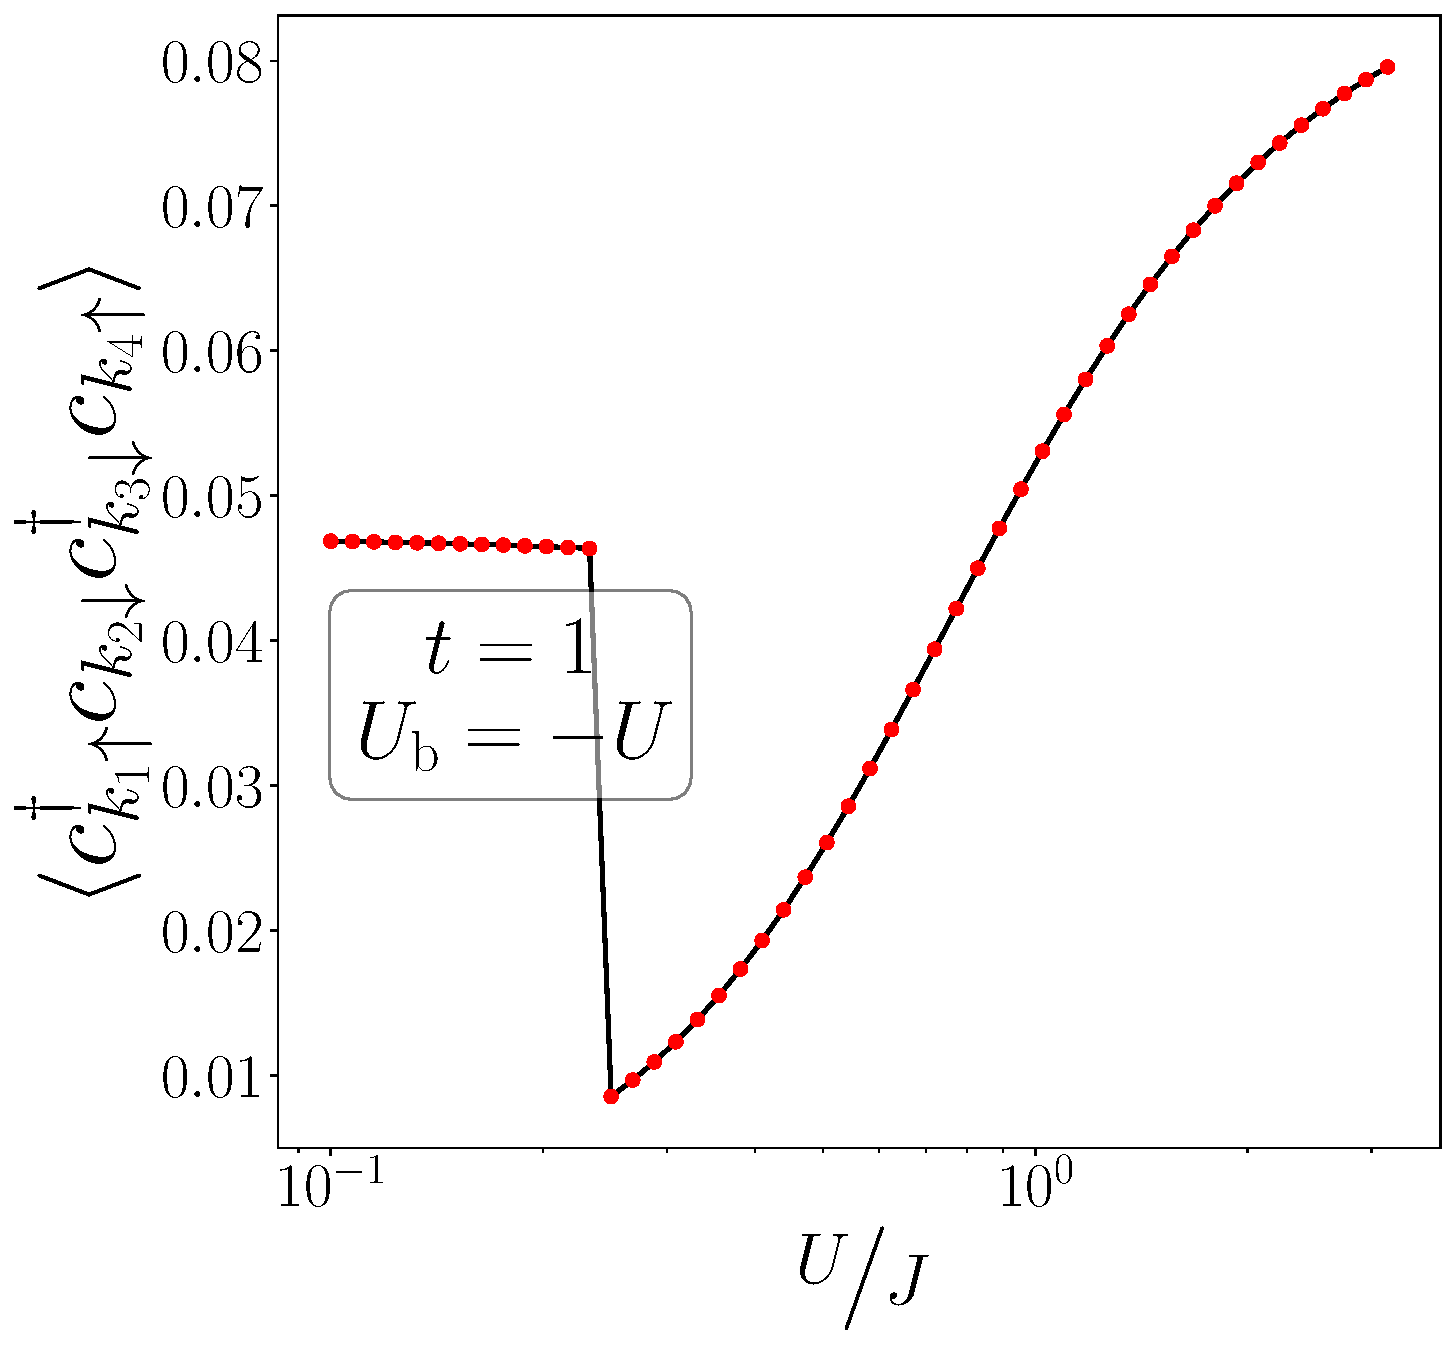
\includegraphics[width=0.24\textwidth]{../figures/corr-k-od-t=1.000,J=100,V=2J,Ubath=-U,N=4,U=0.100,3.162,50.pdf}
\end{center}

\section*{\large Behaviour of mutual information between various real space members}
\begin{center}
	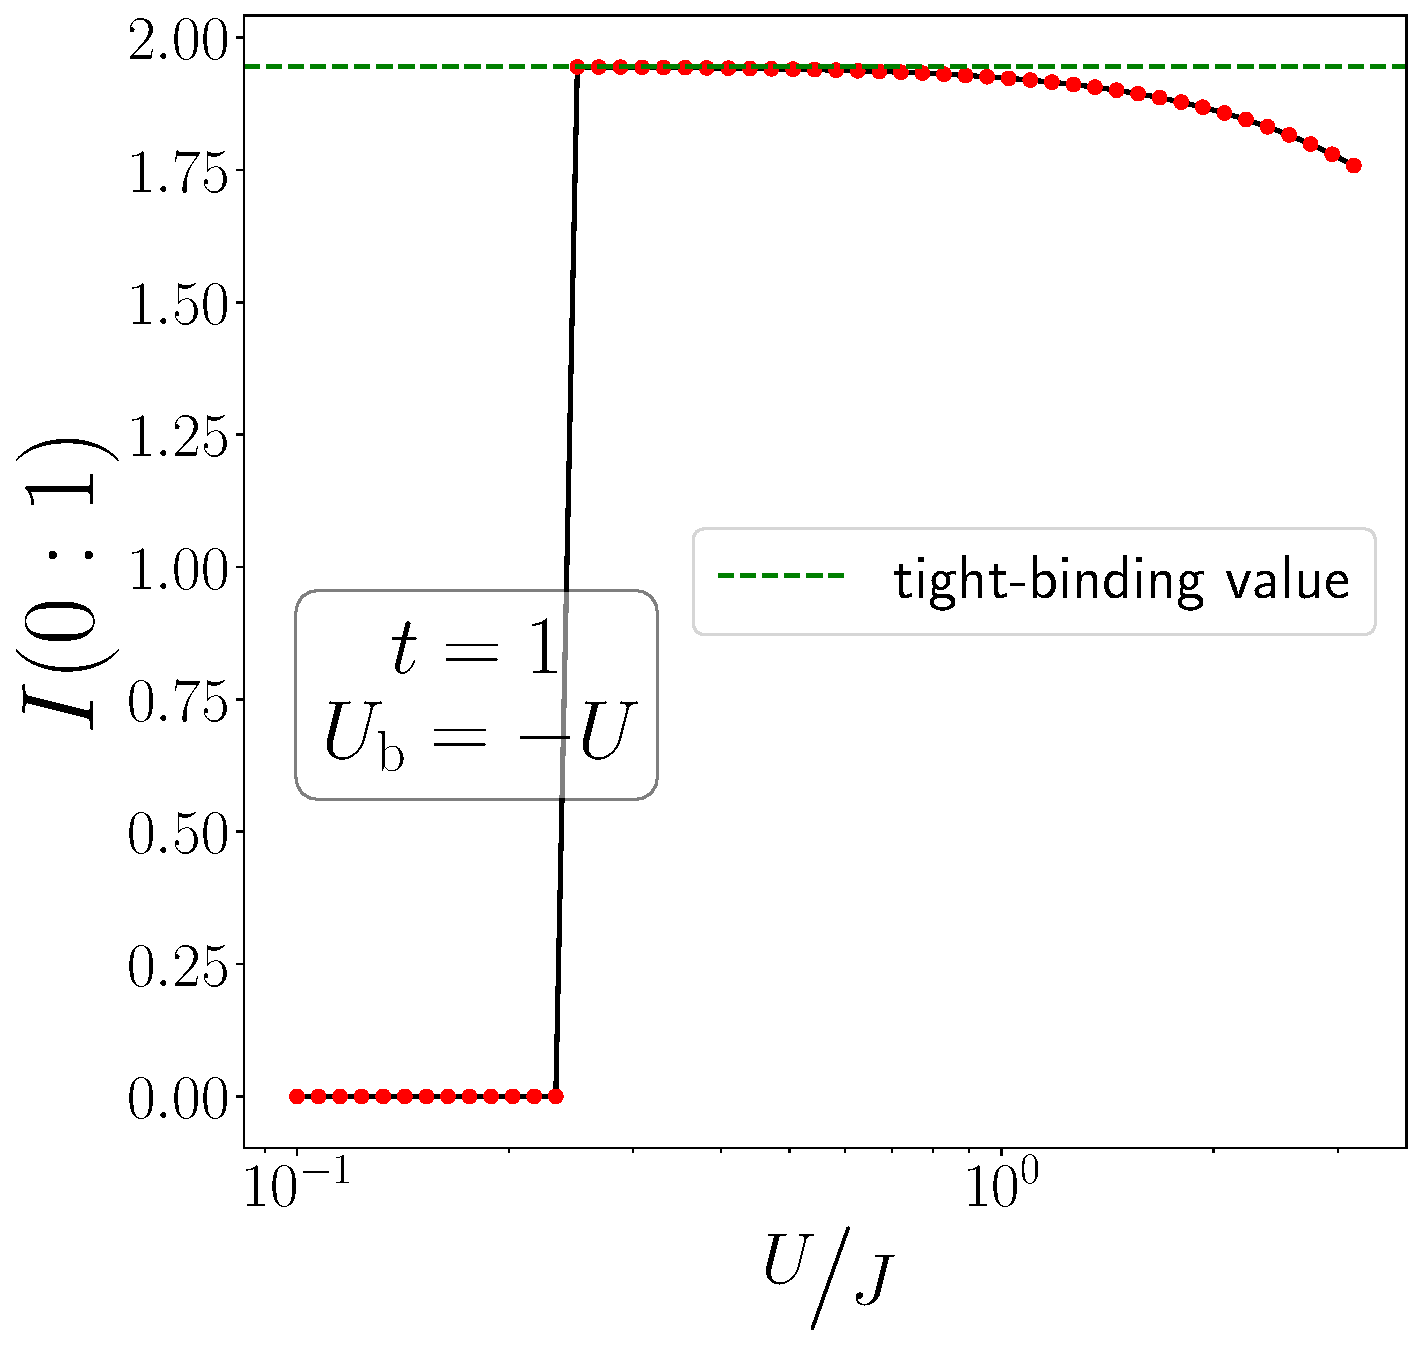
\includegraphics[width=0.32\textwidth]{../figures/mi-01-t=1.000,J=100,V=2J,Ubath=-U,N=4,U=0.100,3.162,50.pdf}
	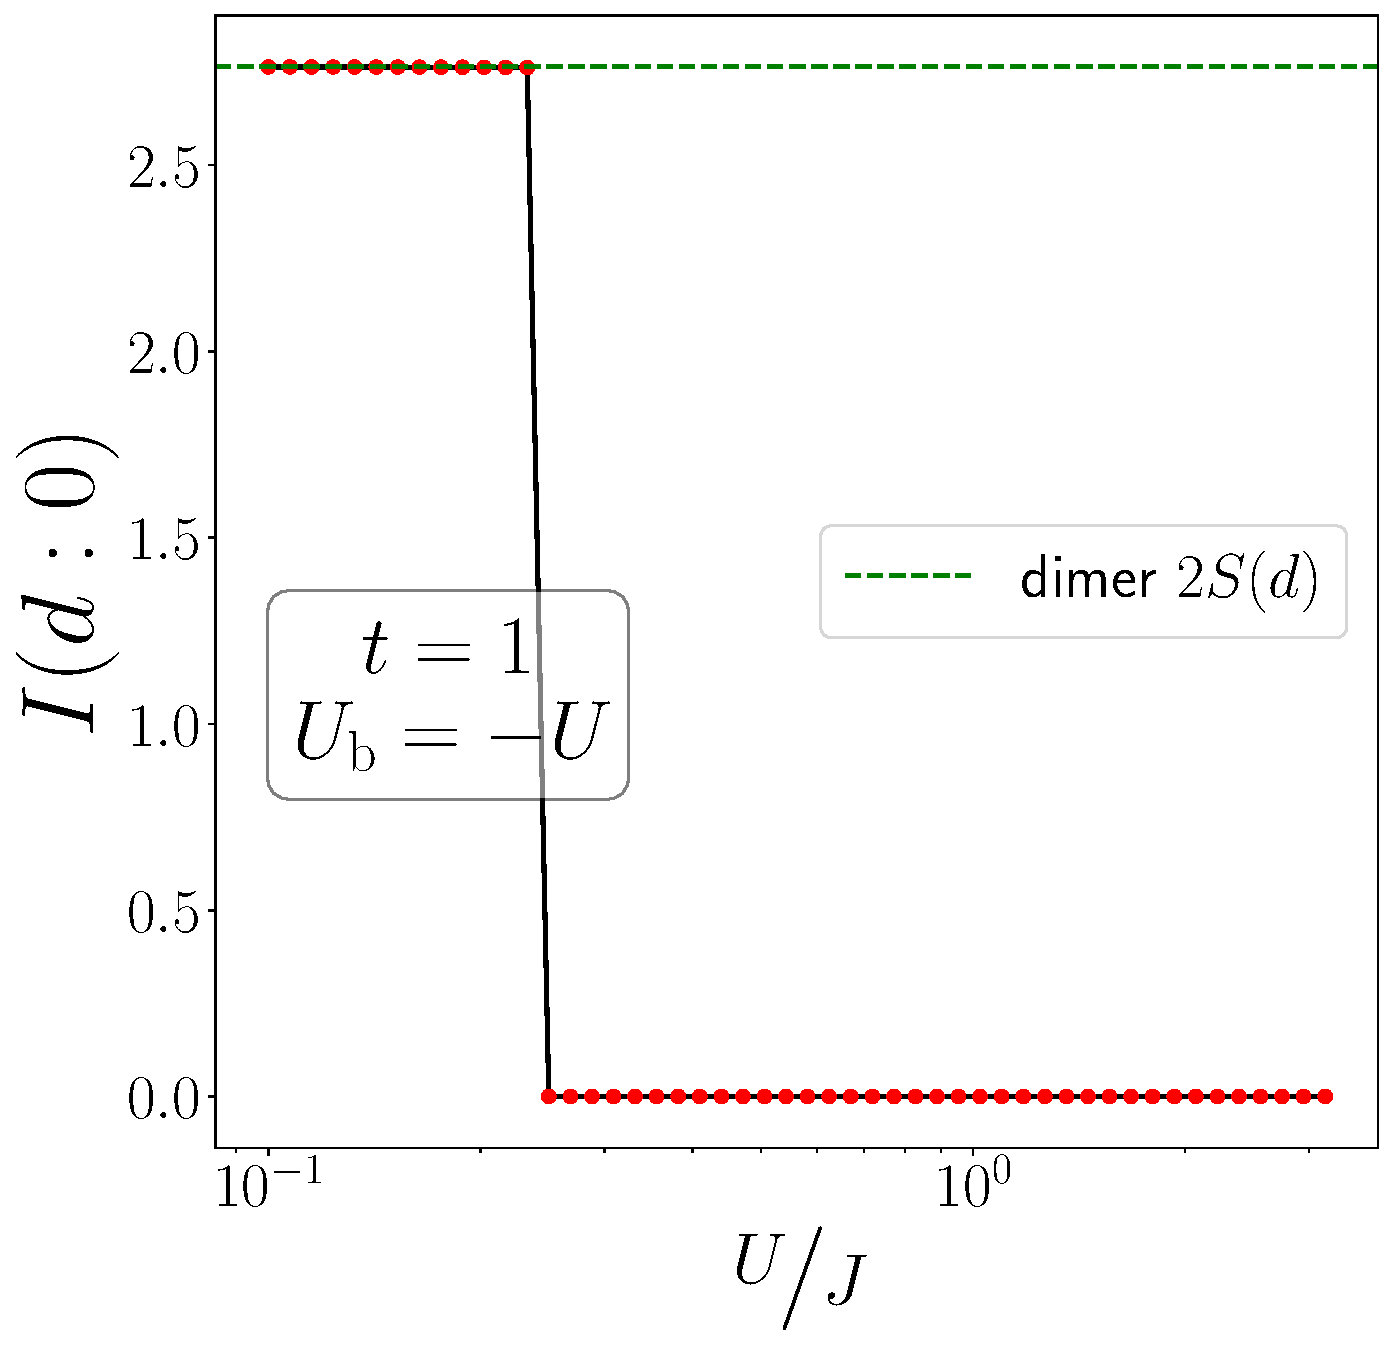
\includegraphics[width=0.32\textwidth]{../figures/mi-d0-t=1.000,J=100,V=2J,Ubath=-U,N=4,U=0.100,3.162,50.pdf}
	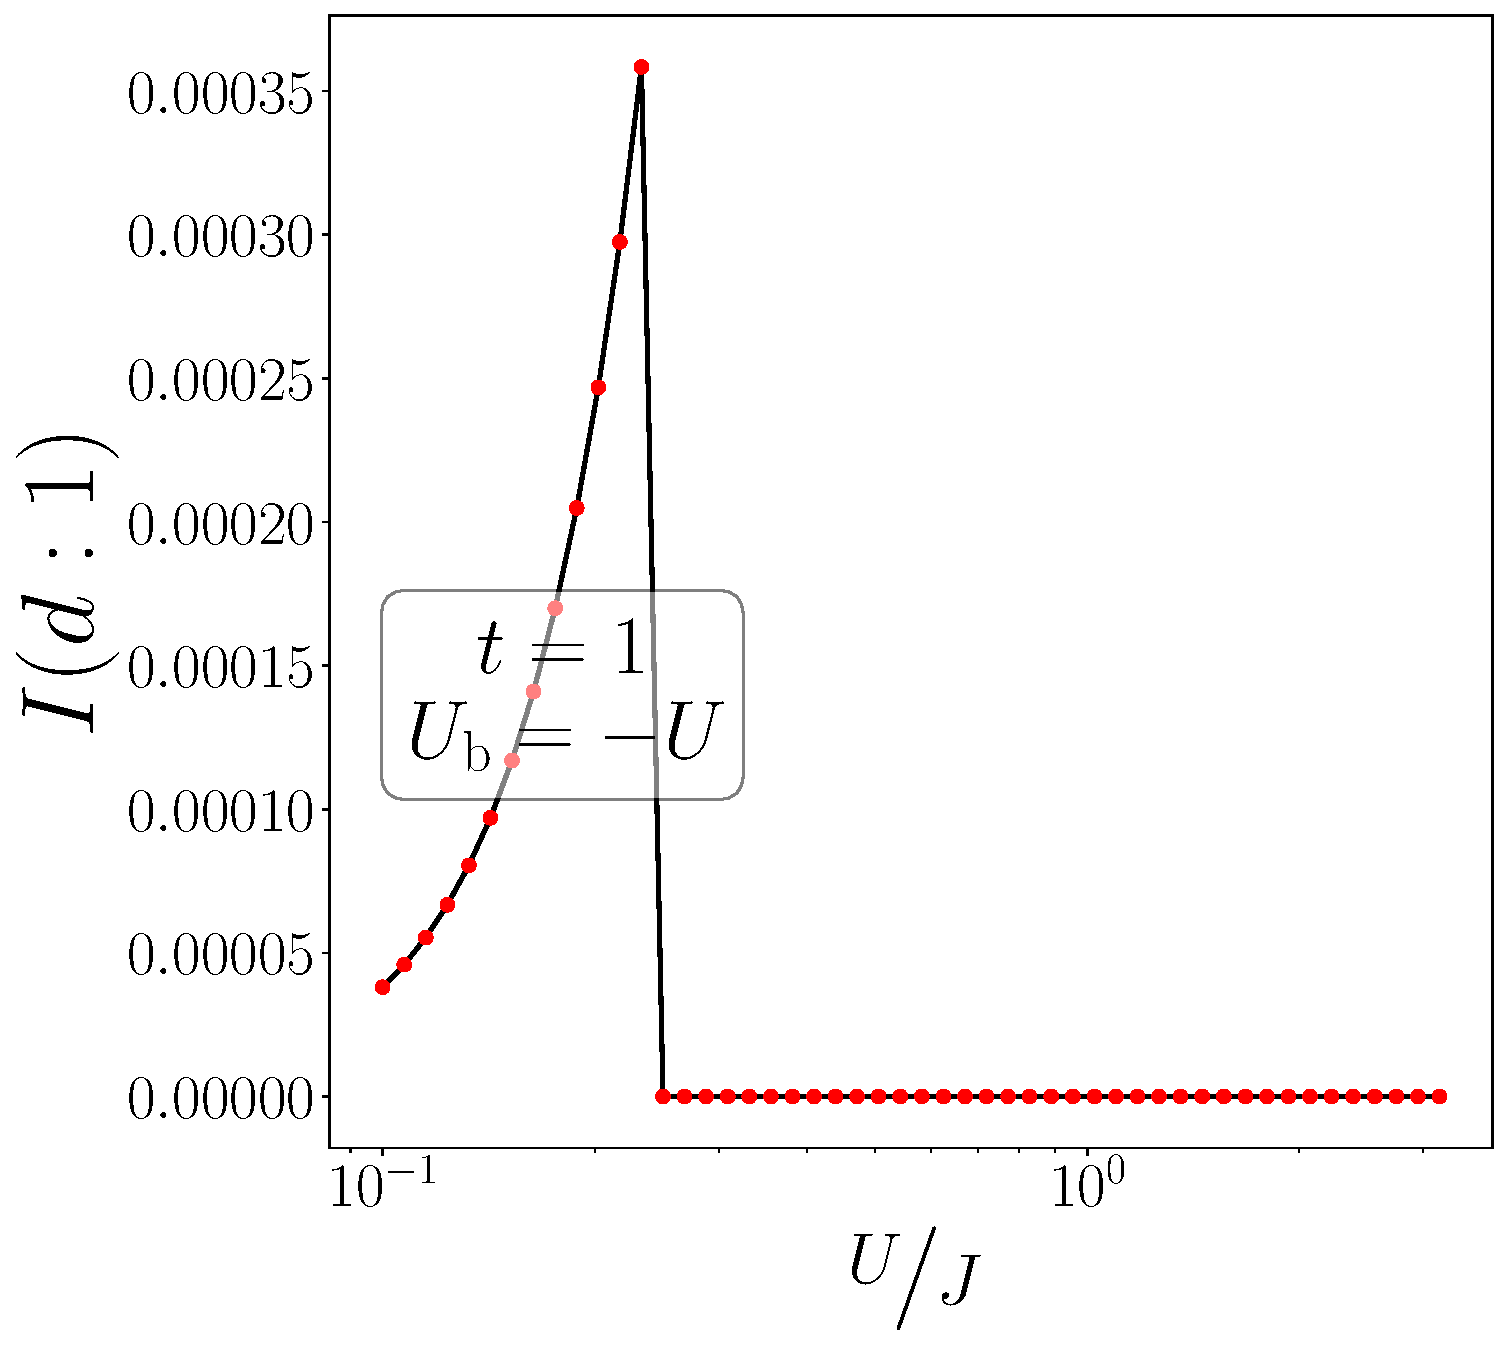
\includegraphics[width=0.32\textwidth]{../figures/mi-d1-t=1.000,J=100,V=2J,Ubath=-U,N=4,U=0.100,3.162,50.pdf}
\end{center}

\section*{\large Behaviour of impurity entanglement entropy and spin-spin correlations}

\begin{center}
	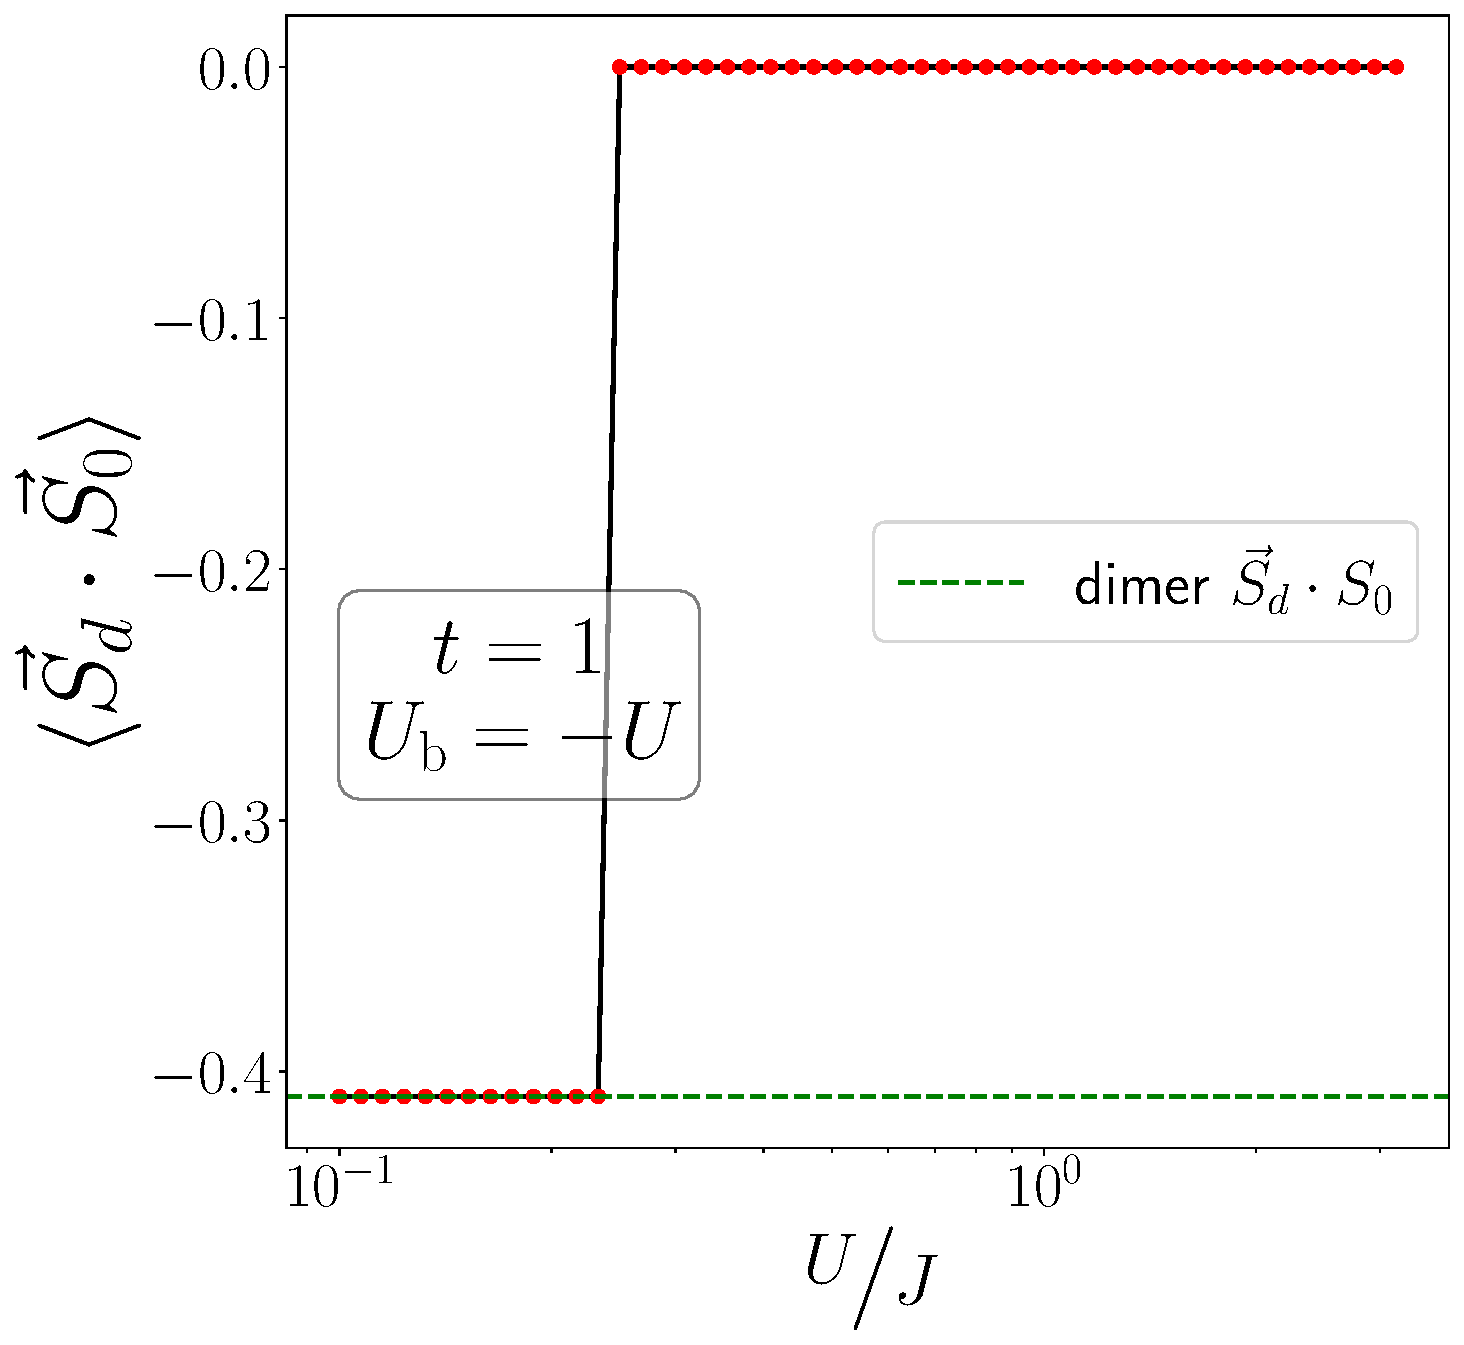
\includegraphics[width=0.32\textwidth]{../figures/corr-d0-t=1.000,J=100,V=2J,Ubath=-U,N=4,U=0.100,3.162,50.pdf}
	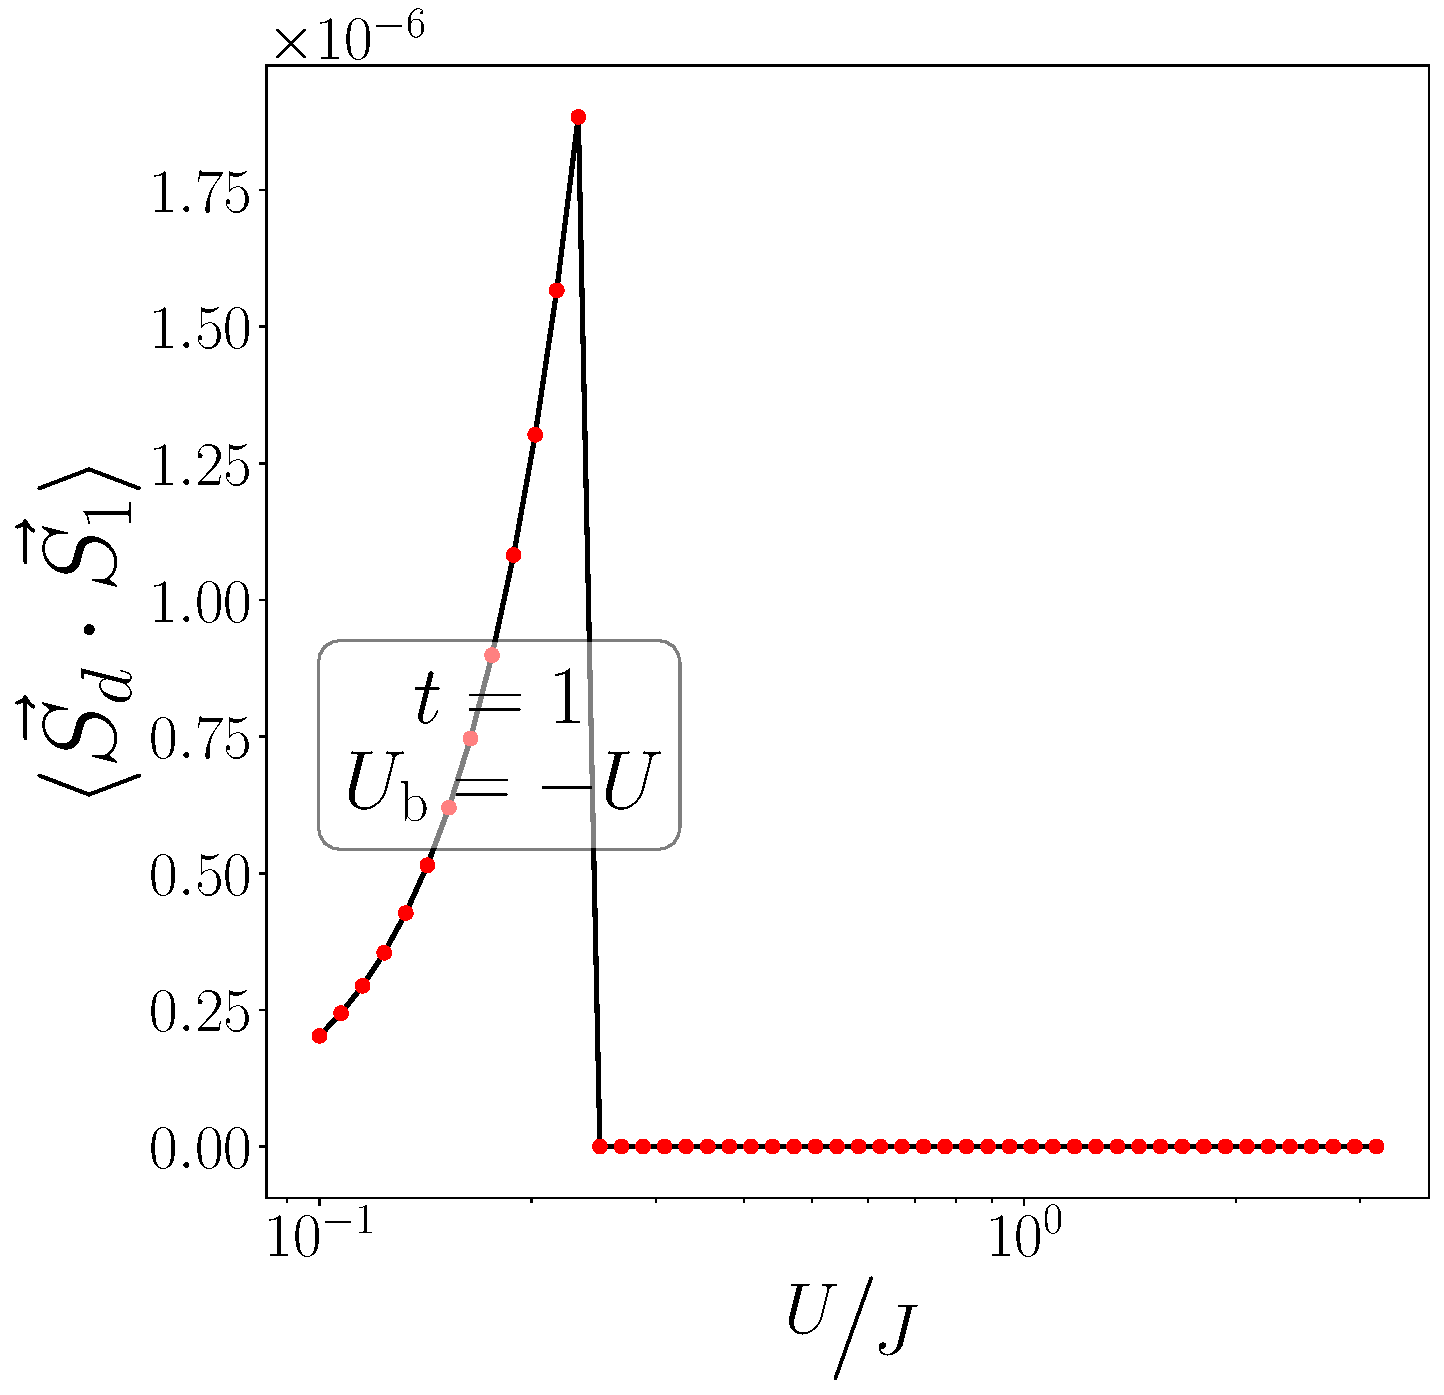
\includegraphics[width=0.32\textwidth]{../figures/corr-d1-t=1.000,J=100,V=2J,Ubath=-U,N=4,U=0.100,3.162,50.pdf}
	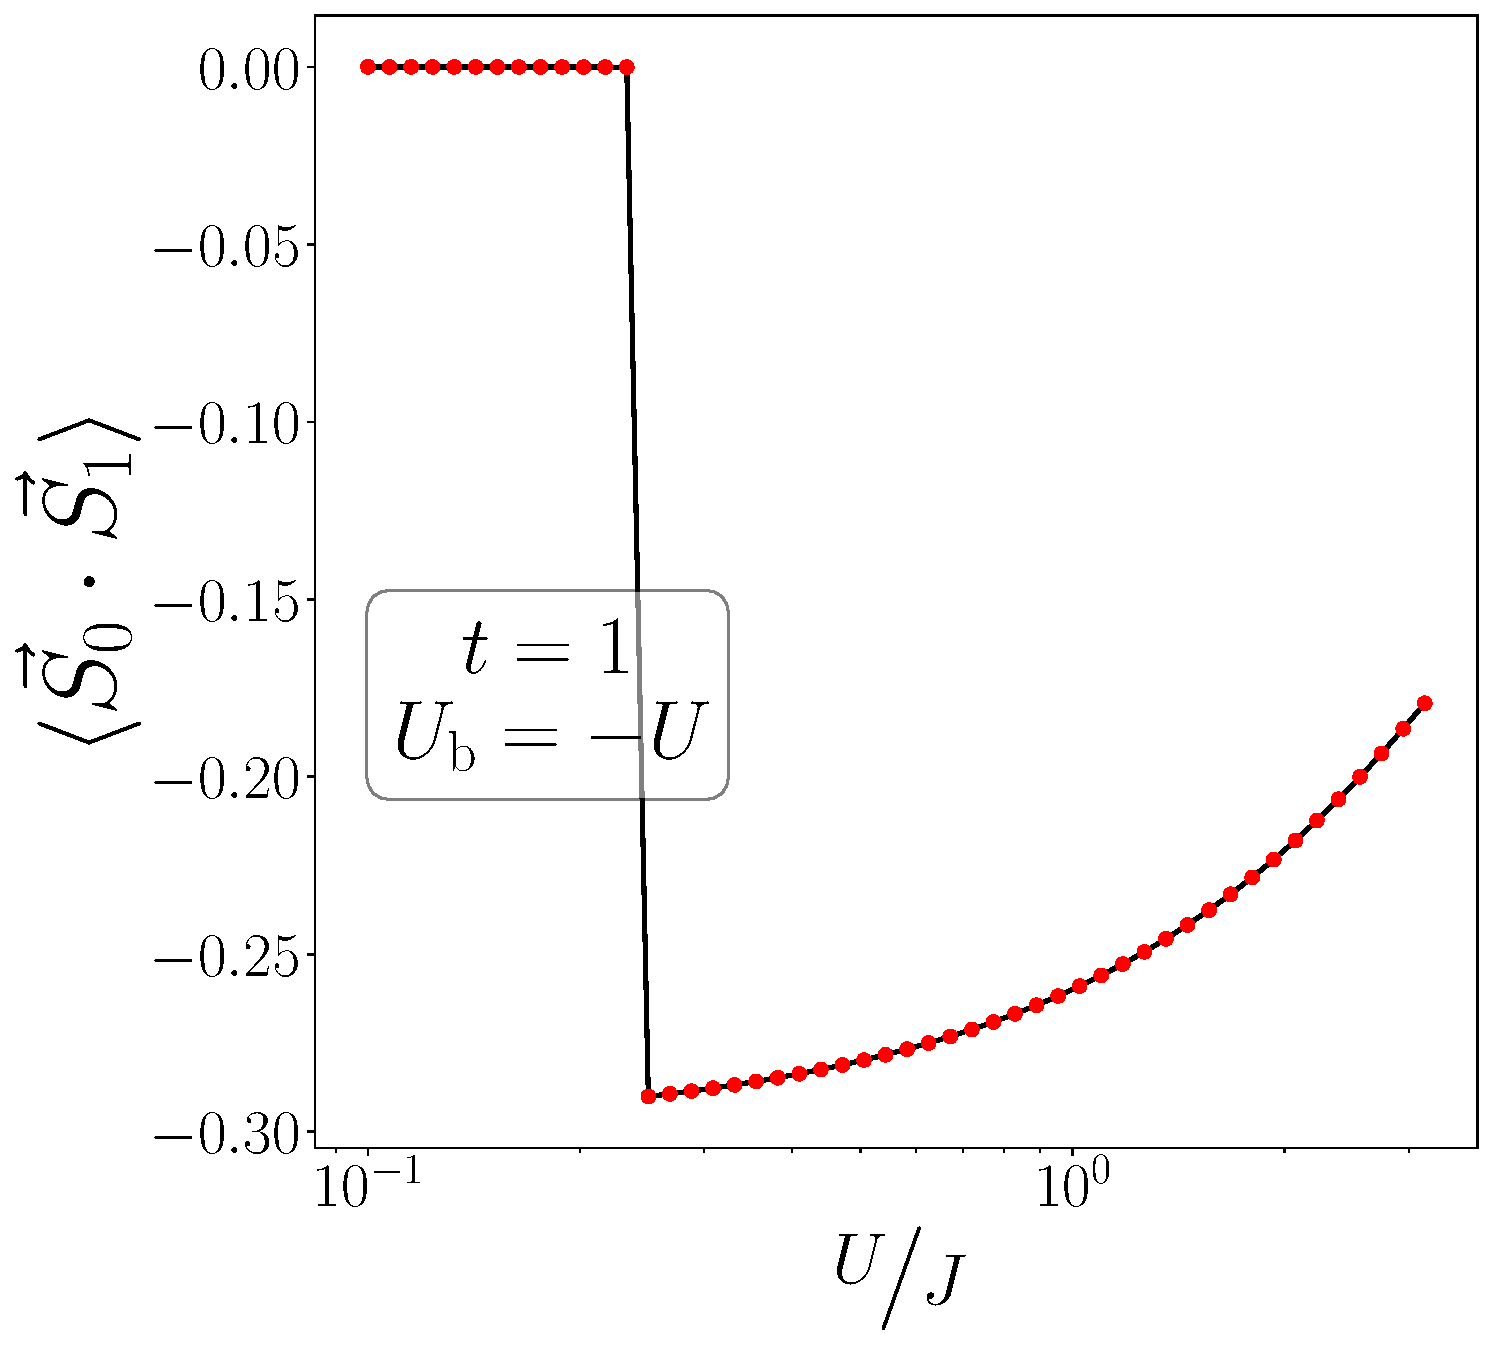
\includegraphics[width=0.32\textwidth]{../figures/r-vec-corr-t=1.000,J=100,V=2J,Ubath=-U,N=4,U=0.100,3.162,50.pdf}

	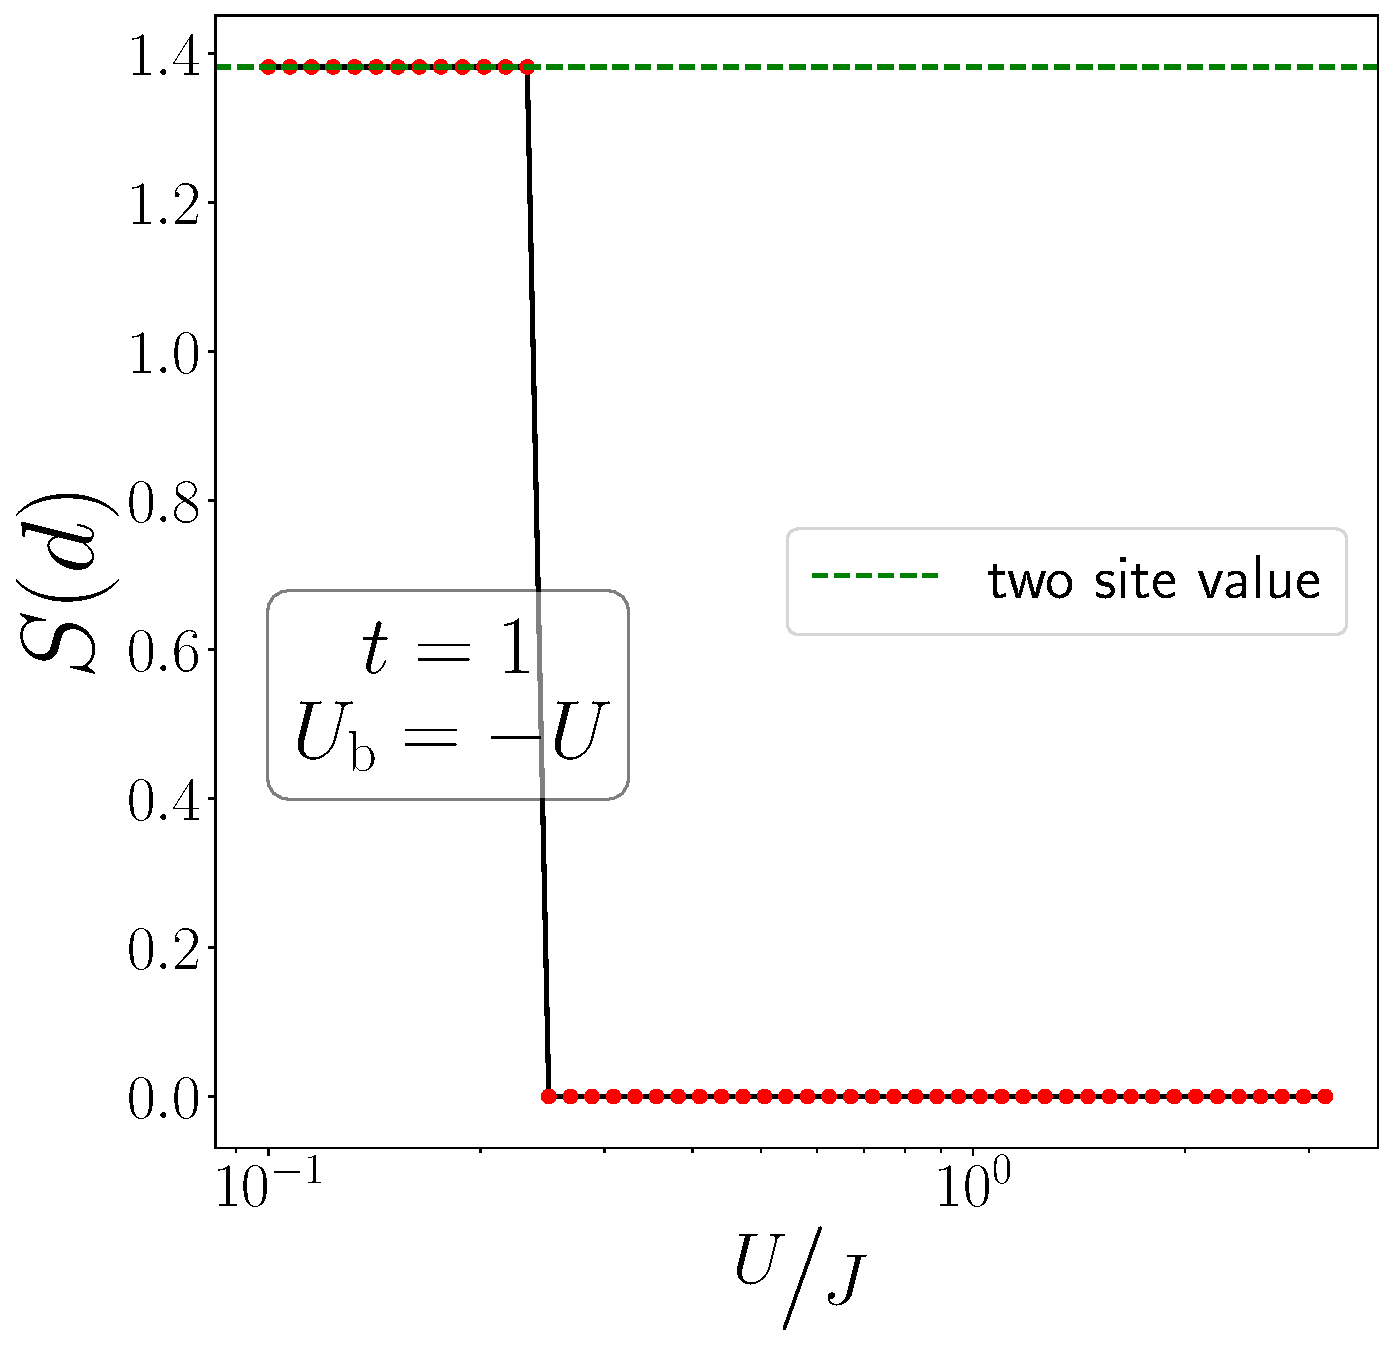
\includegraphics[width=0.32\textwidth]{../figures/EE-d-t=1.000,J=100,V=2J,Ubath=-U,N=4,U=0.100,3.162,50.pdf}
\end{center}

\section*{Behaviour of real-space correlations}
\begin{center}
	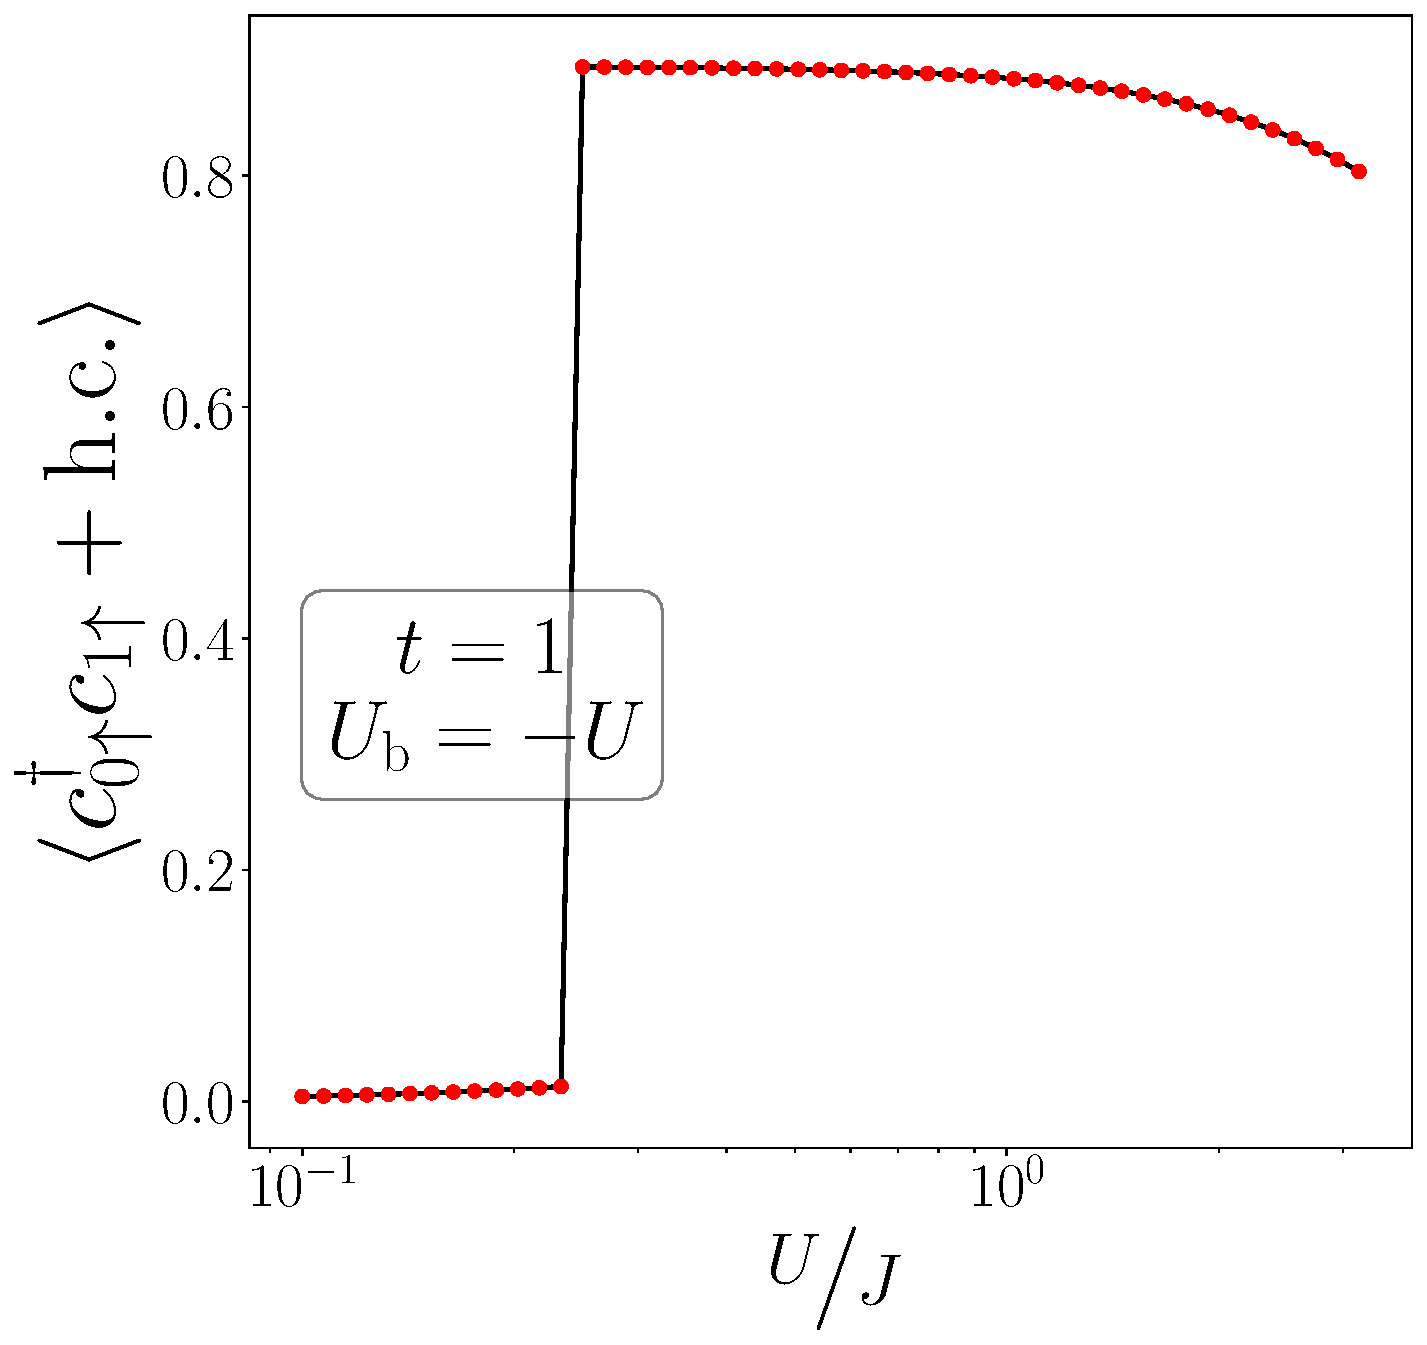
\includegraphics[width=0.32\textwidth]{../figures/r1p-t=1.000,J=100,V=2J,Ubath=-U,N=4,U=0.100,3.162,50.pdf}
	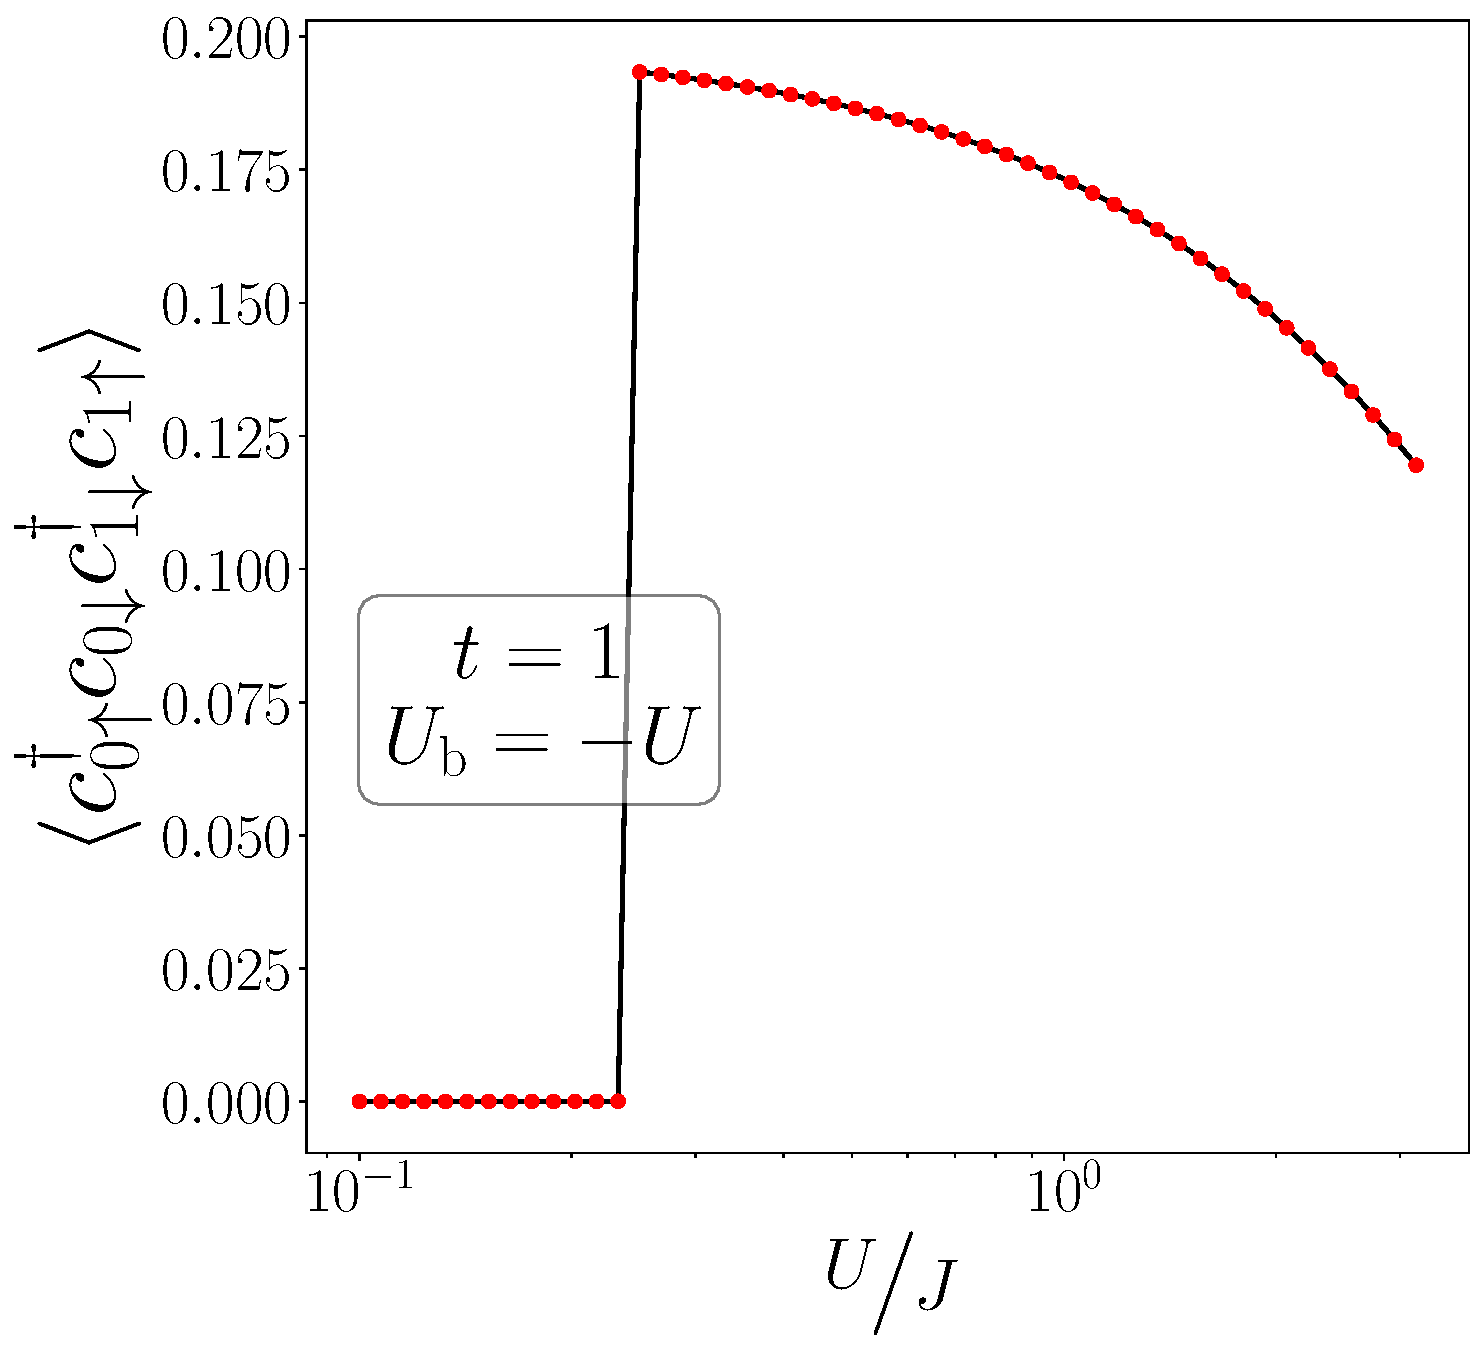
\includegraphics[width=0.32\textwidth]{../figures/r-od-t=1.000,J=100,V=2J,Ubath=-U,N=4,U=0.100,3.162,50.pdf}
	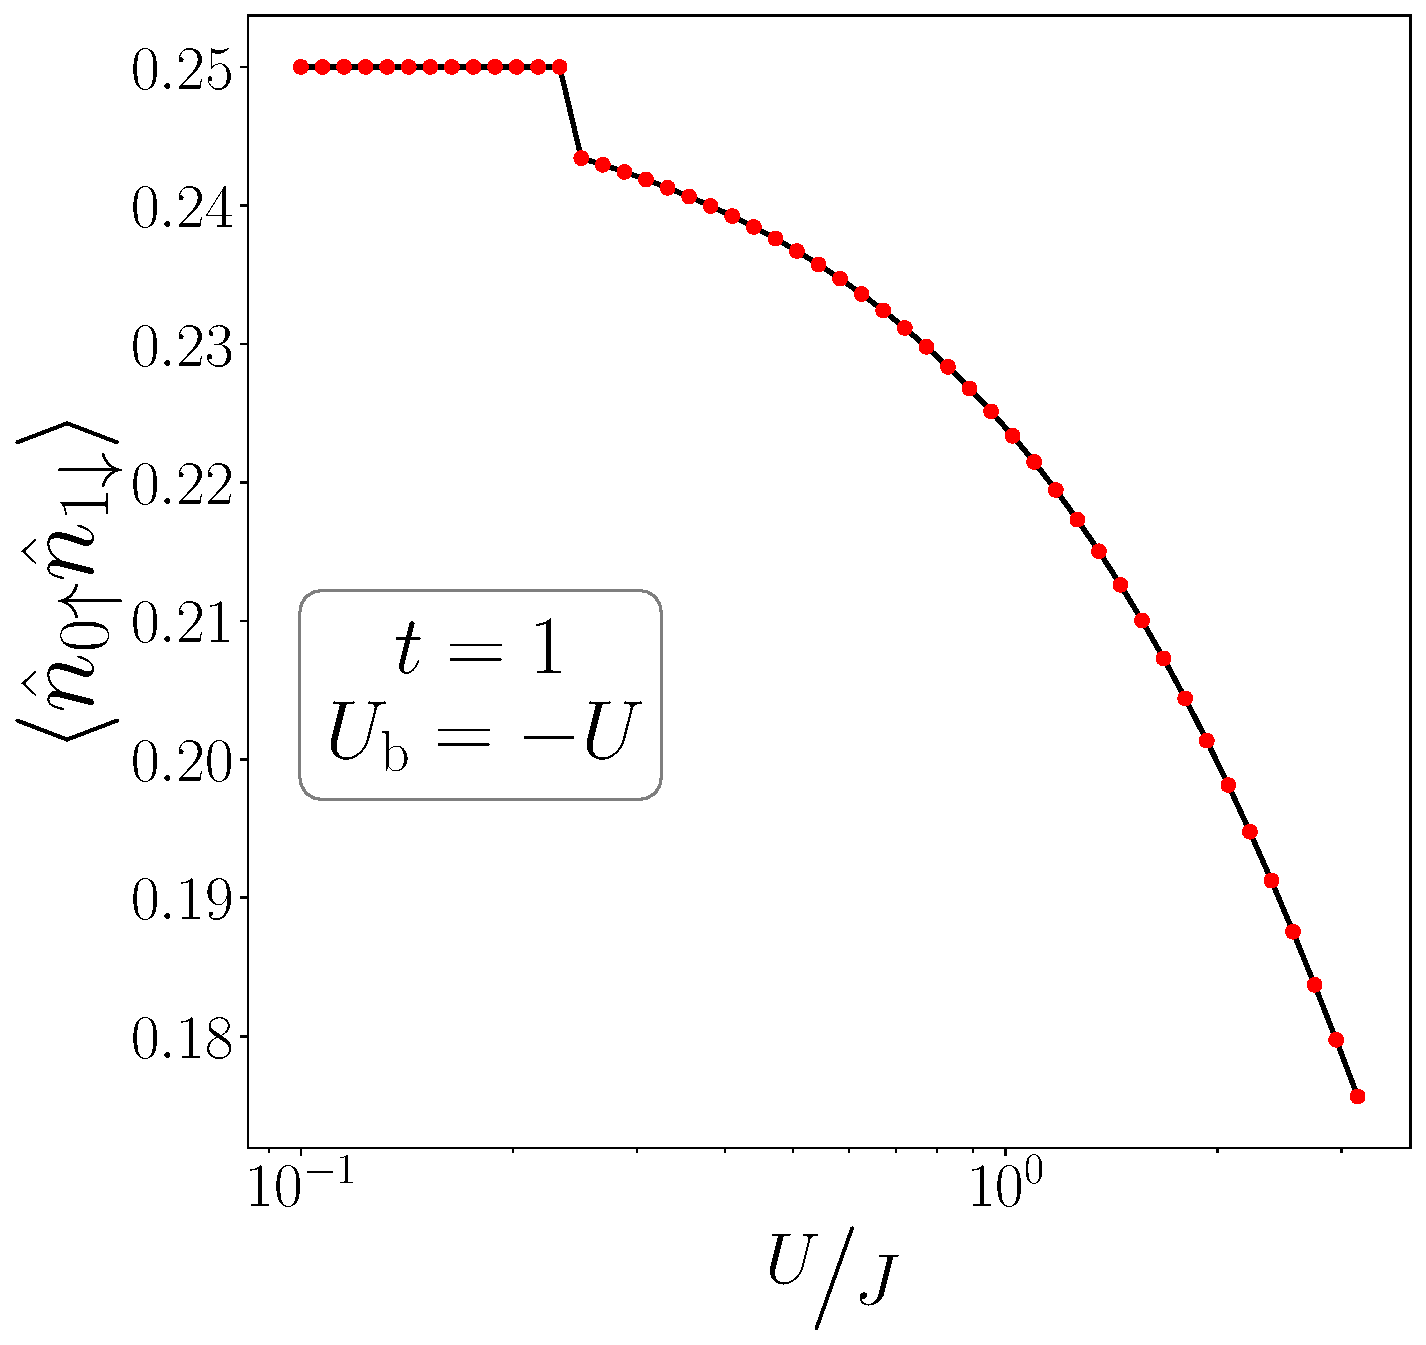
\includegraphics[width=0.32\textwidth]{../figures/r-opp-t=1.000,J=100,V=2J,Ubath=-U,N=4,U=0.100,3.162,50.pdf}

	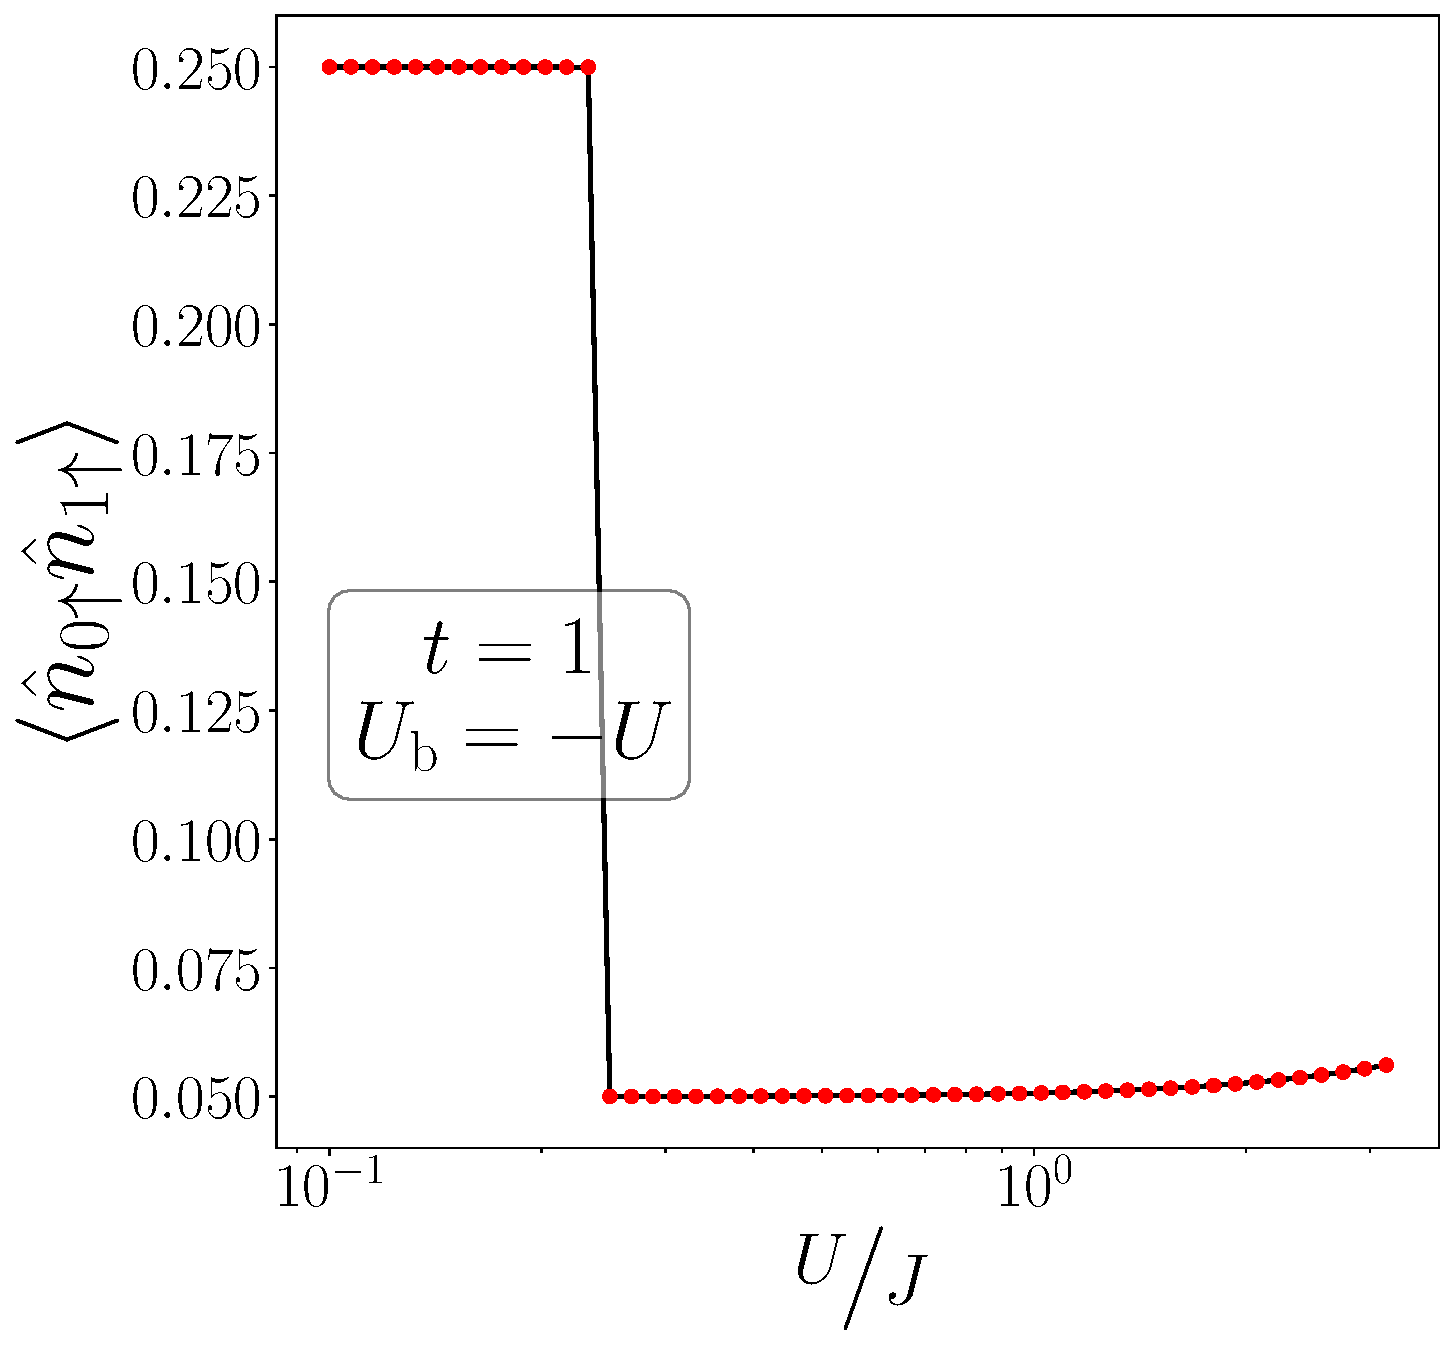
\includegraphics[width=0.3\textwidth]{../figures/r-par-t=1.000,J=100,V=2J,Ubath=-U,N=4,U=0.100,3.162,50.pdf}
	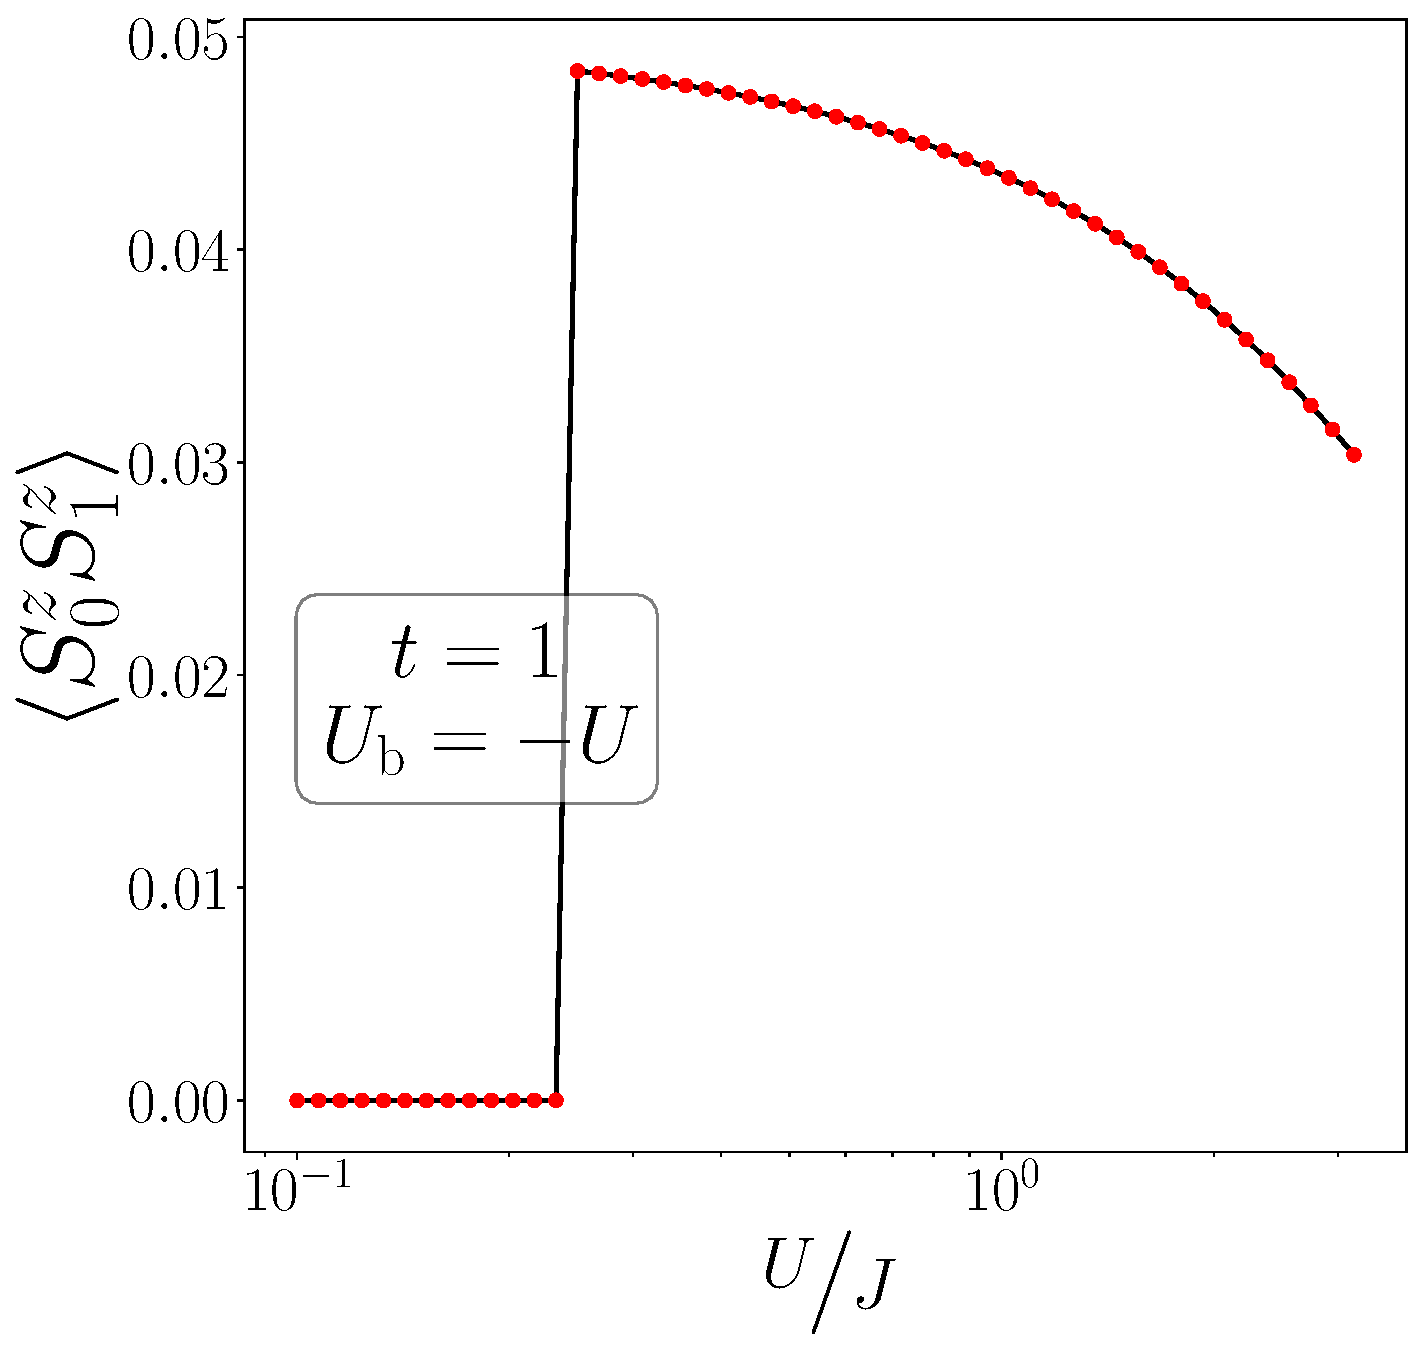
\includegraphics[width=0.3\textwidth]{../figures/r-ising-t=1.000,J=100,V=2J,Ubath=-U,N=4,U=0.100,3.162,50.pdf}
	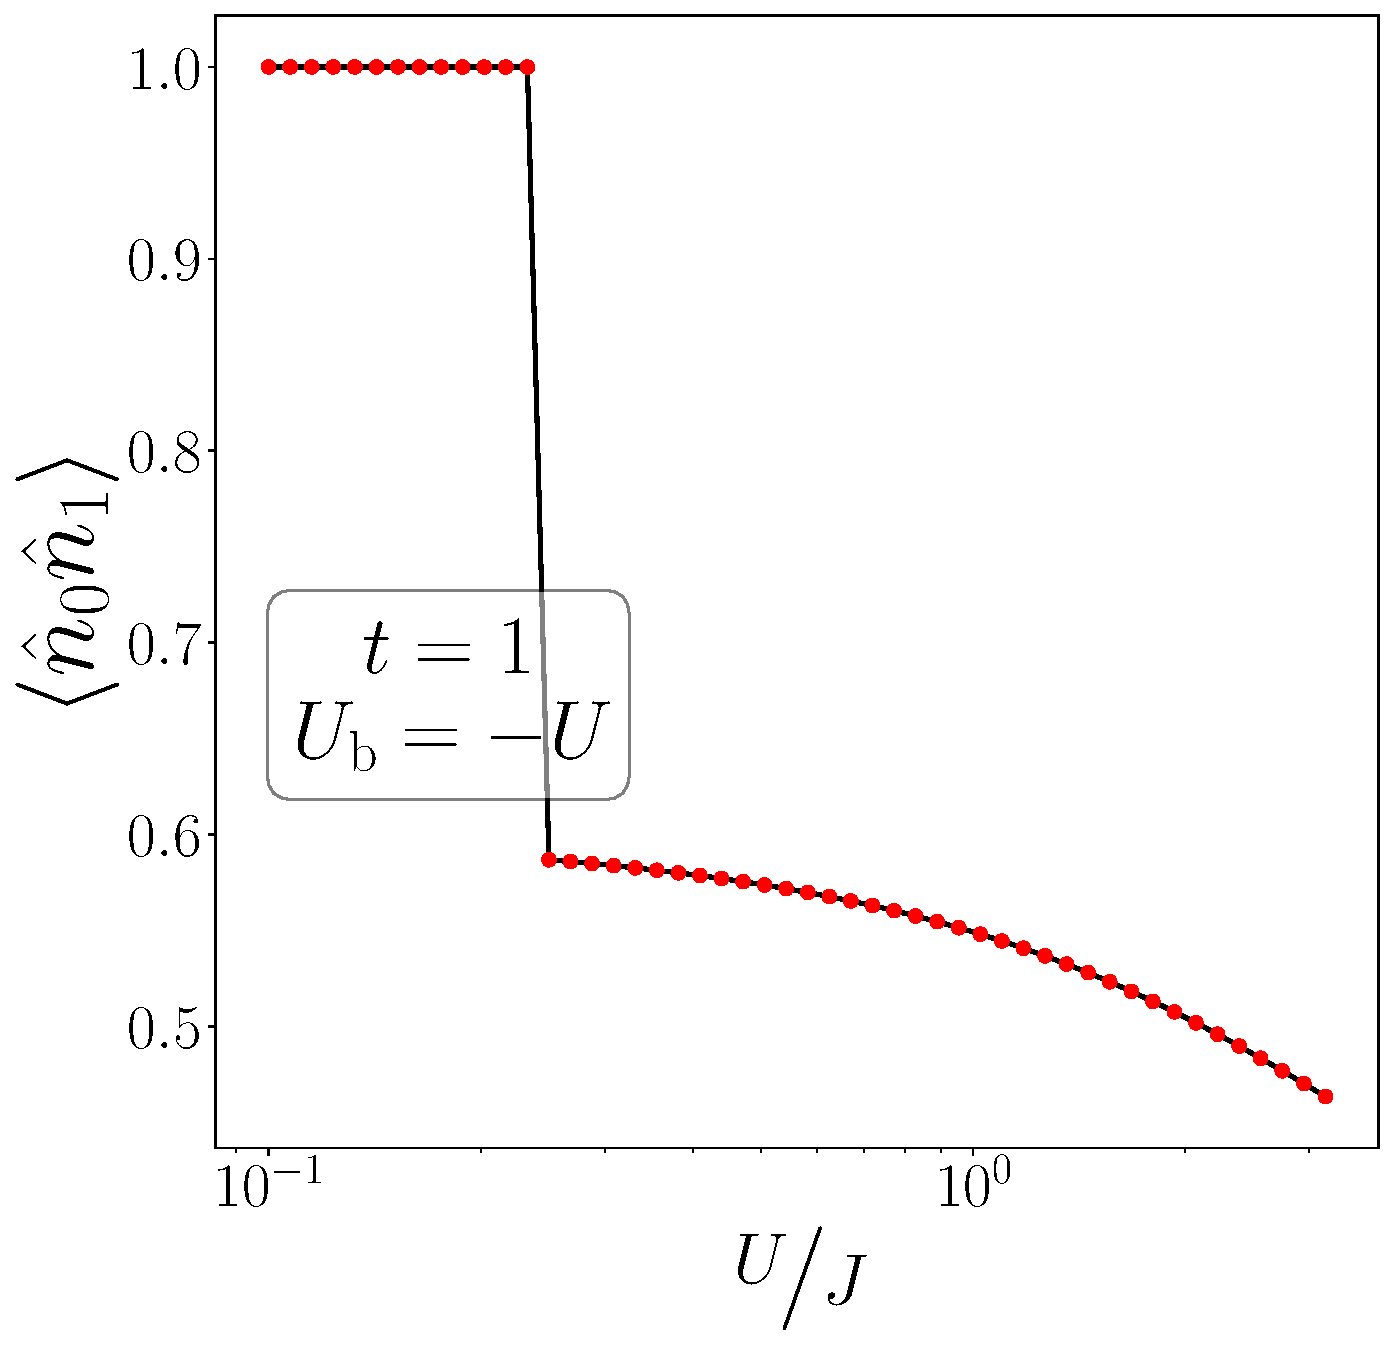
\includegraphics[width=0.3\textwidth]{../figures/r-charge-t=1.000,J=100,V=2J,Ubath=-U,N=4,U=0.100,3.162,50.pdf}
\end{center}

\section*{Impurity spectral function}
\begin{center}
	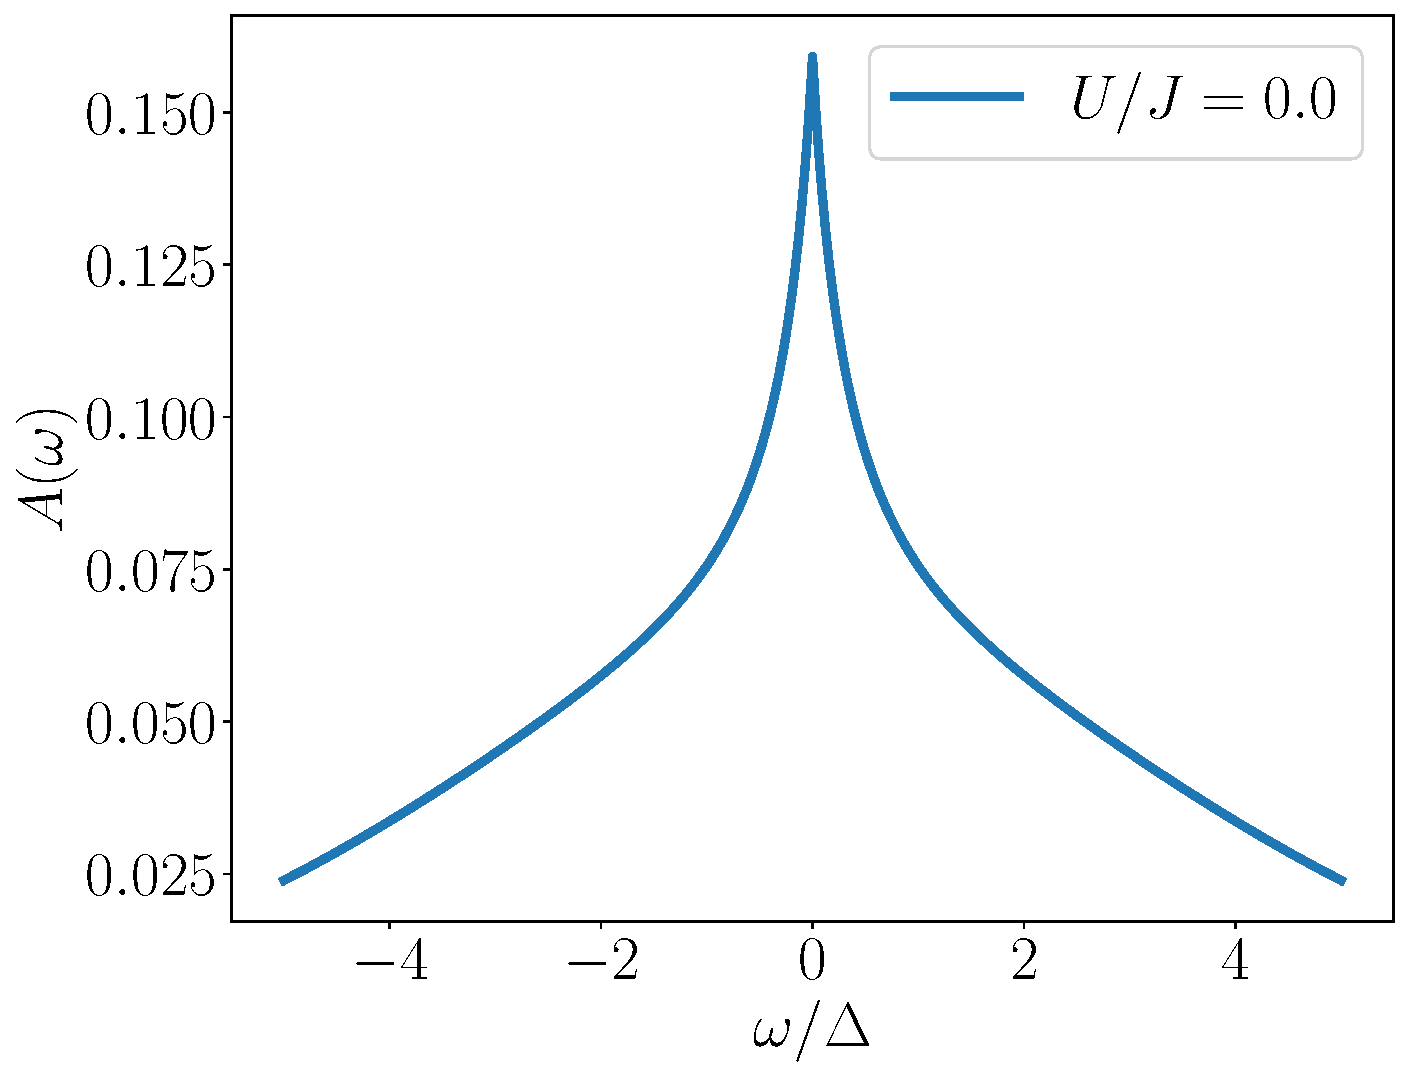
\includegraphics[width=0.45\textwidth]{../figures/spec_func_U_by_J=0.00.pdf}
	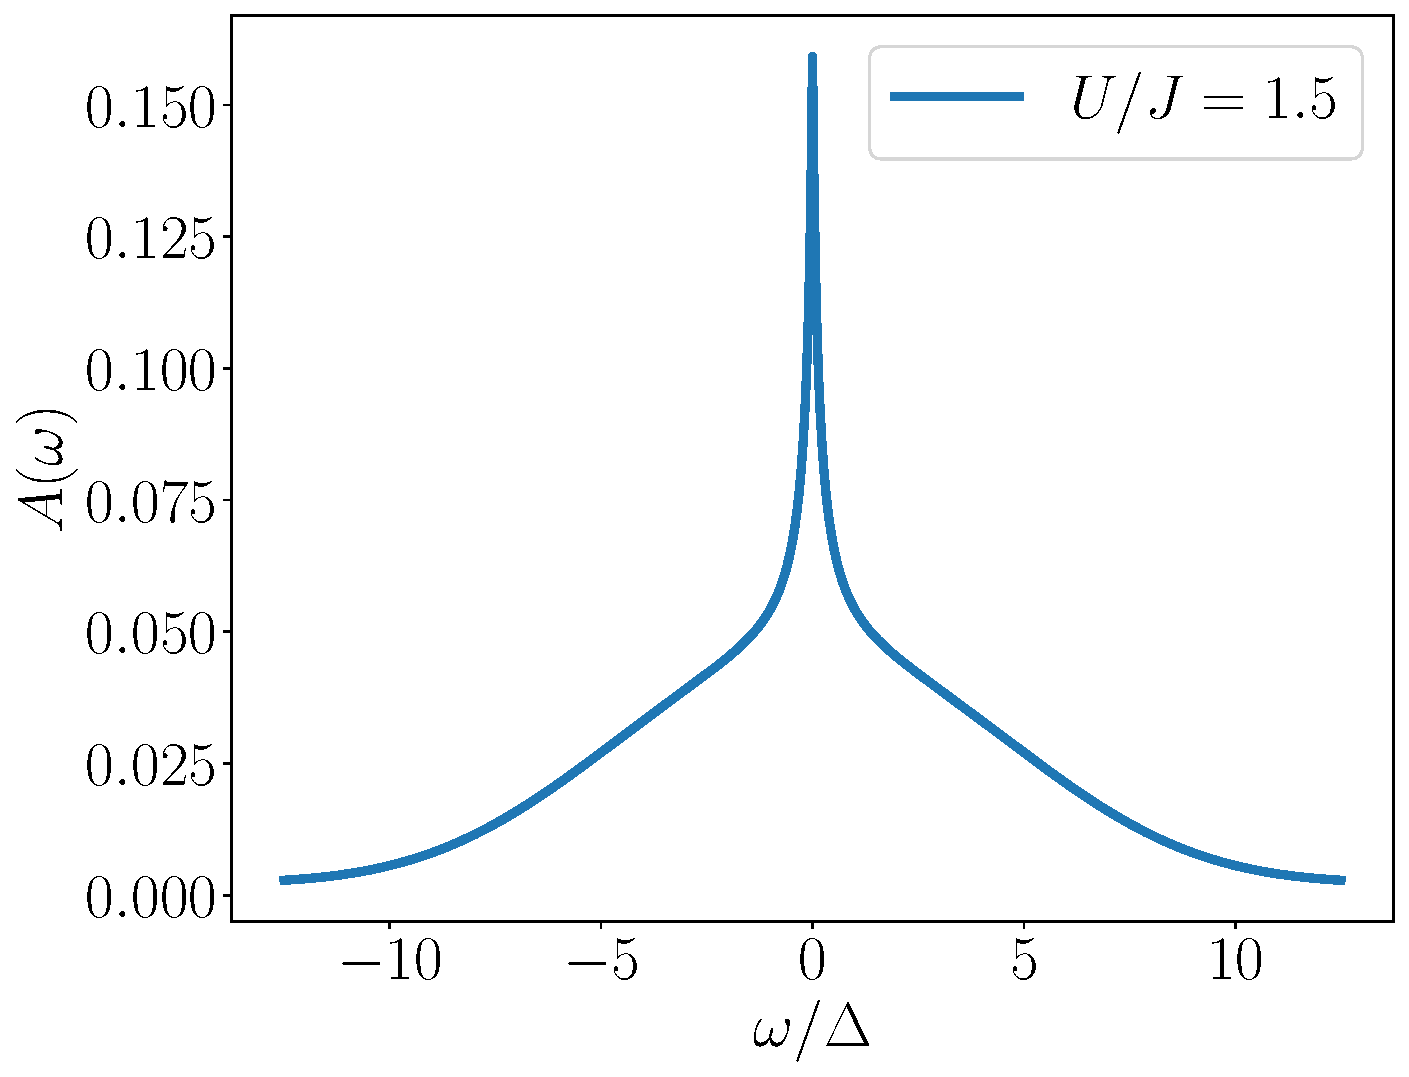
\includegraphics[width=0.45\textwidth]{../figures/spec_func_U_by_J=1.50.pdf}\\
	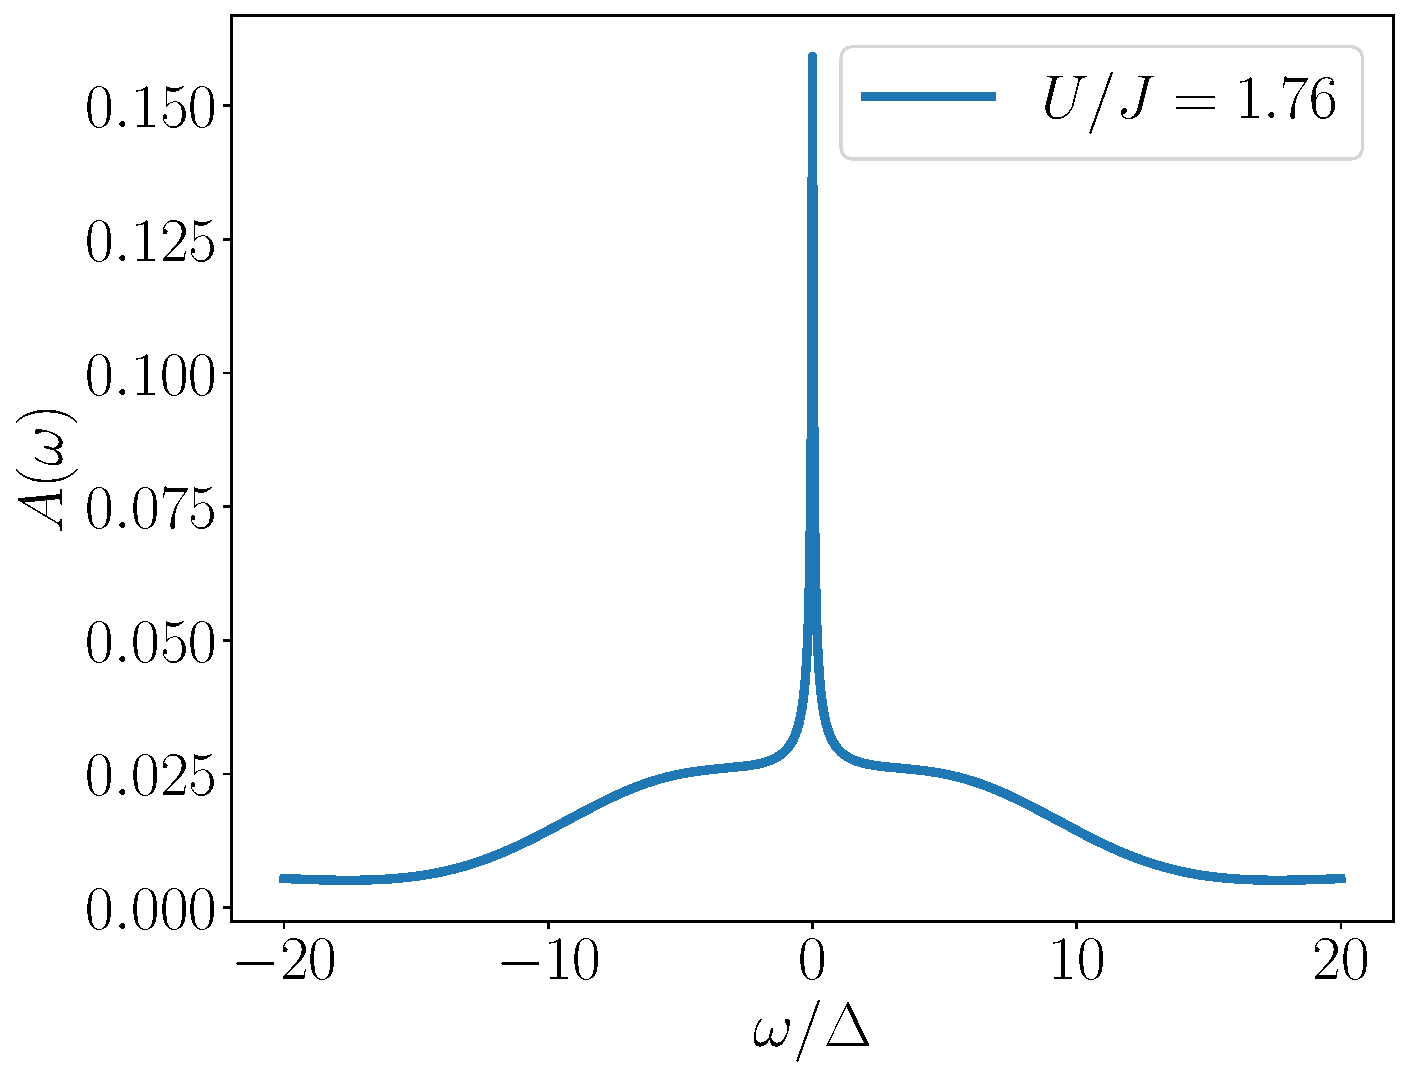
\includegraphics[width=0.45\textwidth]{../figures/spec_func_U_by_J=1.76.pdf}
	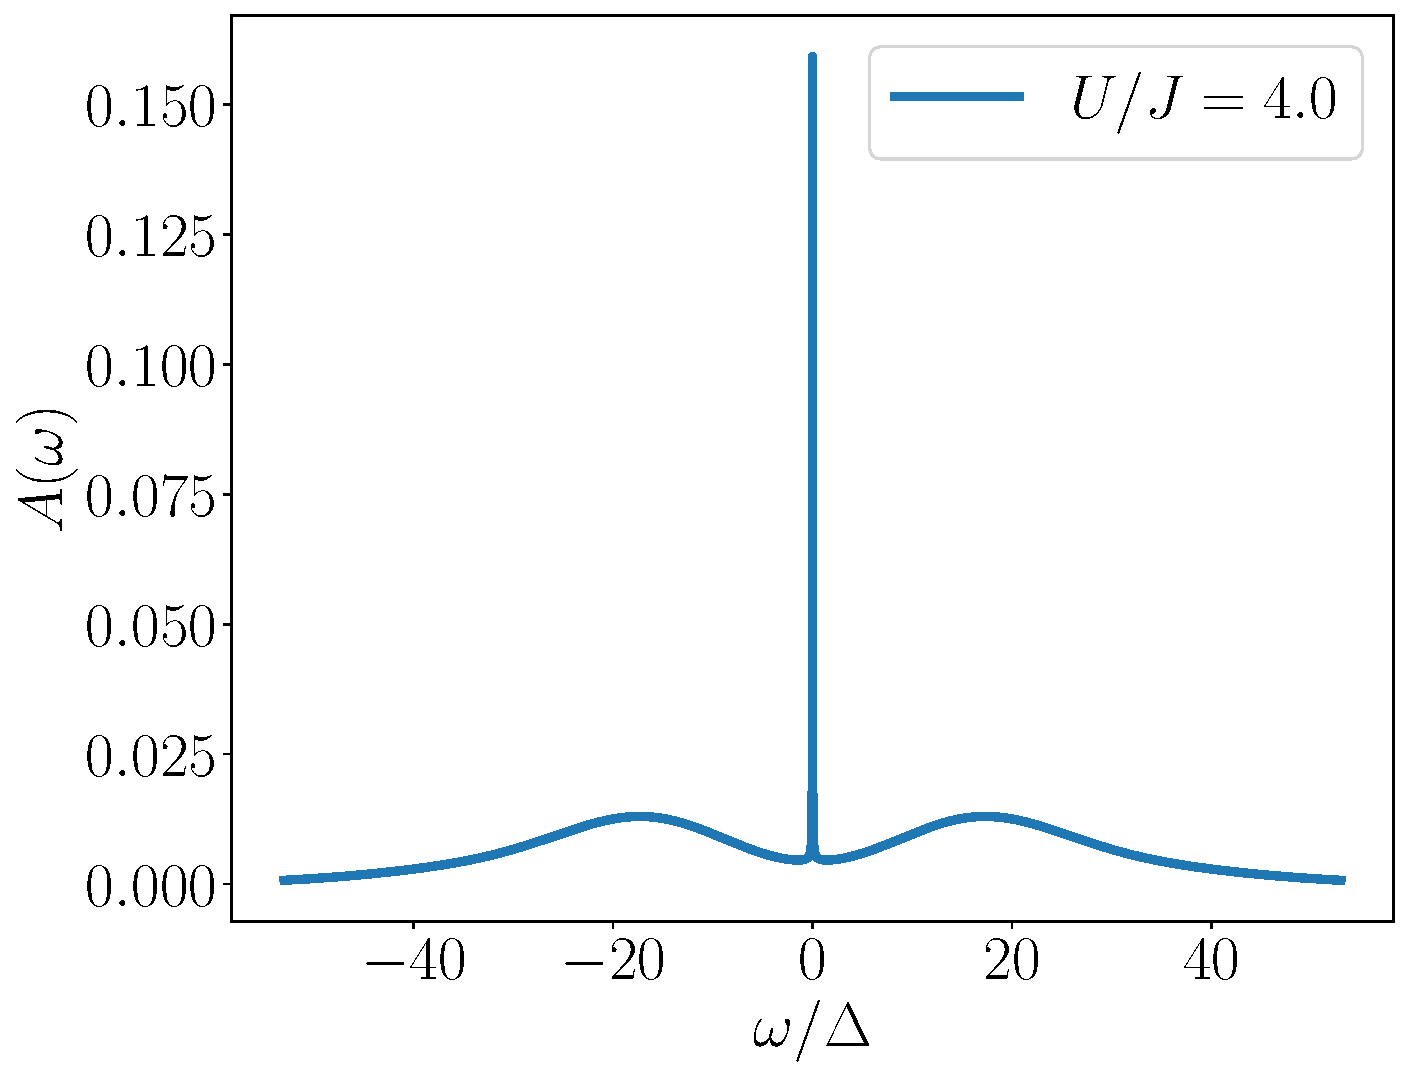
\includegraphics[width=0.45\textwidth]{../figures/spec_func_U_by_J=4.00.pdf}\\
	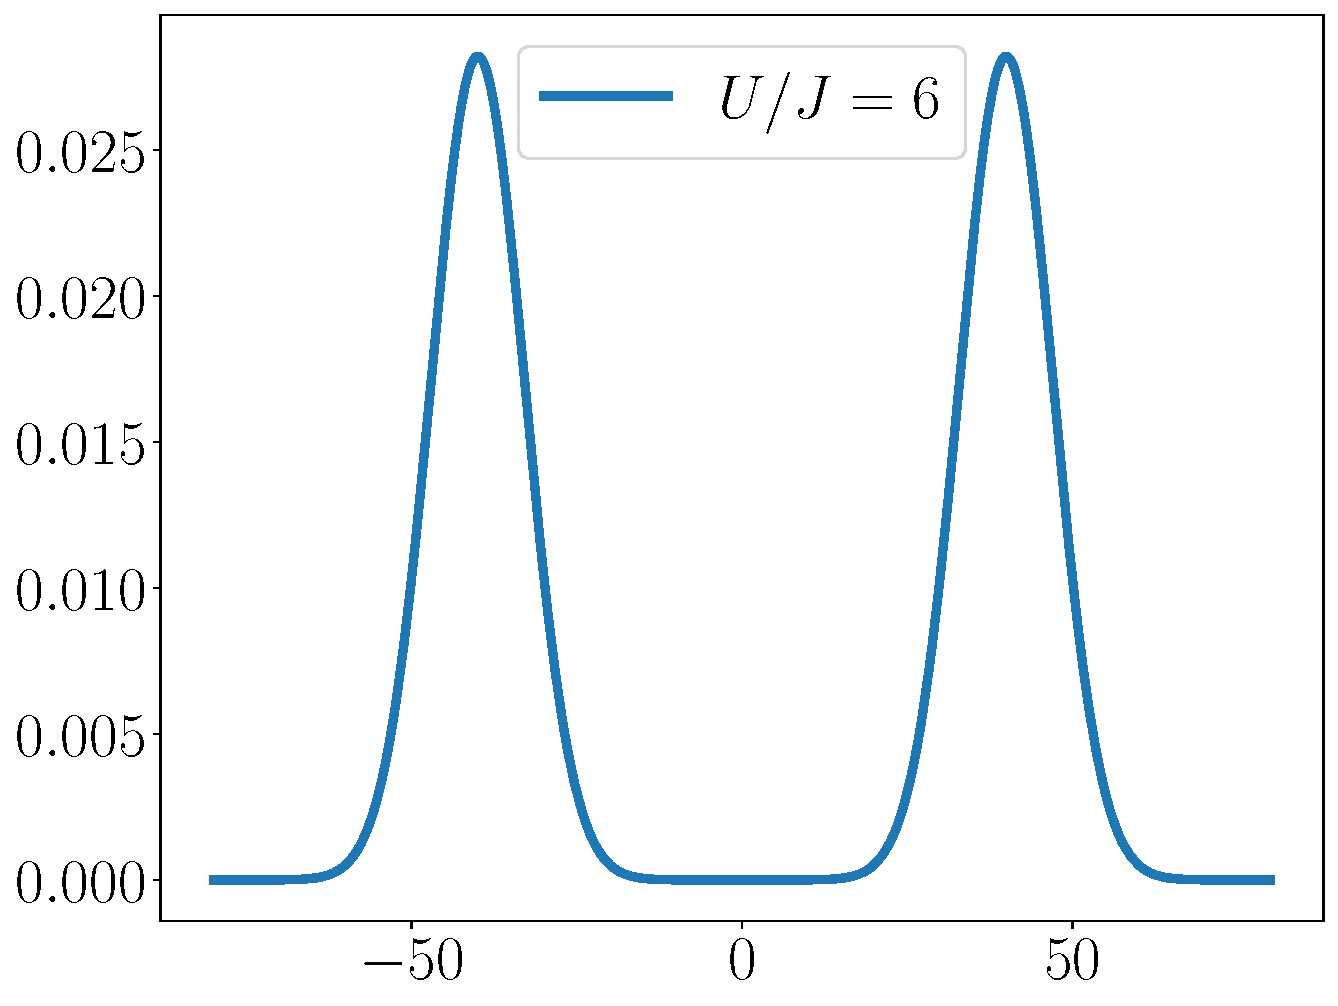
\includegraphics[width=0.45\textwidth]{../figures/spec_func_U_by_J=6.00.pdf}
\end{center}

\section*{Derivation of RG equations}

To treat this under RG, we first Fourier transform this term to \(k-\)space. In \(k-\)space, the diagonal contribution (to \(H_D\)) coming from this term is the single-particle self-energy \(-U_b\left(\hat n_{q \beta}\right)^2\) which can be made particle-hole symmetric in the form:
\begin{equation}\begin{aligned}
	-U_b\left(\tau_{q \beta}\right)^2
\end{aligned}\end{equation}
where \(q\) is the \(k-\)state being decoupled and \(\tau \equiv \hat n - 1/2\). In the initial state \(\ket{\Psi}_i\), we have \(\langle \hat n_{q\beta} \rangle = 1/2 \implies \tau_{q\beta} = 0\), so the contribution of \(U_b\) to that state is 0. For both hole excitations \(c_{q\beta}\ket{\Psi}_i\) as well as particle excitations \(c^\dagger_{q\beta}\ket{\Psi}_i\), the intermediate state energy lowers to \(-U_b/4\).

The off-diagonal part is
\begin{equation}\begin{aligned}
	-\frac{U_b}{2}\sum_{kk^\prime\sigma}c^\dagger_{k\sigma}c_{k^\prime\sigma} + U_b \sum_{k_1,k_2,k_1^\prime,k_2^\prime} c^\dagger_{k_1 \uparrow}c_{k_2 \uparrow} c^\dagger_{k^\prime_1 \downarrow}c_{k^\prime_2 \downarrow} 
\end{aligned}\end{equation}
We ignore the potential scattering arising from the first term.

\subsection*{Renormalisation of \(U_b\)}
\(U_b\) can renormalise only via itself. The relevant renormalisation term in the particle sector is
\begin{equation}\begin{aligned}
	U_b^2 \sum_{q\beta}\sum_{k_1,k_2,k_3,k_1^\prime,k_2^\prime,k_3^\prime} c^\dagger_{q\beta}c_{k_1\beta}c^\dagger_{k_3\overline\beta}c_{k_1^\prime\overline\beta}\frac{1}{\omega - H_D}c^\dagger_{k_2^\prime\overline\beta}c_{k_3^\prime\overline\beta}c^\dagger_{k_2\beta}c_{q\beta}
\end{aligned}\end{equation}
In order to renormalise \(U_b\), we need to contract one more pair of momenta. There are two choices. The first is by setting \(k_3 = k_3^\prime = q\). The two internal states, then, are \(q\beta\) and \(q\overline\beta\). As discussed above, the intermediate state energy is \(-U_b/4\). We therefore have
\begin{equation}\begin{aligned}
	\frac{U_b^2 n_j}{\omega - D/2 + U_b/4}\sum_{\beta}\sum_{k_1,k_2,k_1^\prime,k_2^\prime} c_{k_1\beta}c_{k_1^\prime\overline\beta}c^\dagger_{k_2^\prime\overline\beta}c^\dagger_{k_2\beta} = \frac{U_b^2 n_j}{\omega - D/2 + U_b/4}\sum_{\beta}\sum_{k_1,k_2,k_1^\prime,k_2^\prime} c^\dagger_{k_2^\prime\overline\beta}c_{k_1^\prime\overline\beta}c^\dagger_{k_2\beta}c_{k_1\beta}
\end{aligned}\end{equation}
Another way to contract the momenta is by setting \(k_1^\prime = k_2^\prime = q\), which gives a renormalisation of
\begin{equation}\begin{aligned}
	\frac{U_b^2 n_j}{\omega - D/2 + U_b/4}\sum_{\beta}\sum_{k_1,k_2,k_3,k_3^\prime} c_{k_1\beta}c^\dagger_{k_3 \overline\beta}c_{k_3\prime\overline\beta}c^\dagger_{k_2\beta} = -\frac{U_b^2 n_j}{\omega - D/2}\sum_{\beta}\sum_{k_1,k_2,k_3,k_3^\prime} c^\dagger_{k_3 \overline\beta}c_{k_3\prime\overline\beta}c^\dagger_{k_2\beta}c_{k_1\beta}
\end{aligned}\end{equation}
The two contributions cancel each other. The same cancellation happens in the hole sector as well.

\subsection*{Renormalisation of \(U\)}
\(U_b\) does not have any new renormalisation term on account of \(U_b\). \(U_b\) does however modify the existing RG equation for \(U\), by shifting the denominator. The existing RG equation is
\begin{equation}\begin{aligned}
	\Delta U &= -4V^2 n_j\left(\frac{1}{\omega - \frac{D}{2} + \epsilon_d + \frac{K}{4}} - \frac{1}{\omega - \frac{D}{2} - \epsilon_d + \frac{J}{4}}\right) - n_j\left(\frac{J^2}{\omega - \frac{D}{2} + \frac{J}{4}} - \frac{K^2}{\omega - \frac{D}{2} + \frac{K}{4}}\right)~.
\end{aligned}\end{equation}
On accounting for the contribution of \(U_b\) to the denominator, we get
\begin{equation}\begin{aligned}
	\Delta U &= -4V^2 n_j\left(\frac{1}{\omega - \frac{D}{2} + \frac{U_b}{4} + \epsilon_d + \frac{K}{4}} - \frac{1}{\omega - \frac{D}{2} + \frac{U_b}{4} - \epsilon_d + \frac{J}{4}}\right) - n_j\left(\frac{J^2}{\omega - \frac{D}{2} + \frac{U_b}{4} + \frac{J}{4}} - \frac{K^2}{\omega - \frac{D}{2} + \frac{U_b}{4} + \frac{K}{4}}\right)~.
\end{aligned}\end{equation}

\subsection*{Renormalisation of \(V\)}
The single-particle  hybridisation \(V\) renormalises through terms of \(V U_b\) and \(U_b V\) kind. The first term gives
\begin{equation}\begin{aligned}
	&\sum_{q\beta}\sum_{k}U_b V c^\dagger_{q\beta}c_{k\beta} \hat n_{q\overline\beta} \frac{1}{\omega - H_D} c^\dagger_{d\beta}c_{q\beta} \\
	&= n_jU_b V\sum_{k\beta} c_{k\beta} \left[\frac{\hat n_{d\overline\beta}}{2}\left(\frac{1}{\omega_1 - E_1} + \frac{1}{\omega^\prime_1 - E_1}\right) + \frac{1-\hat n_{d\overline\beta}}{2}\left(\frac{1}{\omega_0 - E_0} + \frac{1}{\omega_0^\prime - E_0}\right)\right] c^\dagger_{d\beta}
\end{aligned}\end{equation}
\(E_1\) and \(E_0\) are the intermediate state energies for \(\hat n_{d\overline\beta}=1\) and 0 respectively. \(\omega_{1,0}\) are the quantum fluctuation scales for the corresponding initial states. \(\omega^\prime_{1,0}\) are the fluctuation scales for the corresponding final states.
The intermediate energies are \(E_1 = D/2 - U_b/4 - K/4,~ ~ ~ E_0 = D/2 - U_b/4 - U/2 - J/4\). The fluctuation scales are \(\omega_1 = \omega - U/2= \omega_0^\prime,~ ~ ~ \omega_1^\prime = \omega = \omega_0\). Substituting these gives
\begin{equation}\begin{aligned}
	-n_jU_b V\sum_{k\beta} c^\dagger_{d\beta} c_{k\beta} \left[\frac{\hat n_{d\overline\beta}}{2}\left(\frac{1}{\omega - \frac{D}{2} - \frac{U}{2} + \frac{U_b}{4} + \frac{K}{4}} + \frac{1}{\omega - \frac{D}{2} + \frac{U_b}{4} + \frac{K}{4}}\right) \right.\\
+\left. \frac{1-\hat n_{d\overline\beta}}{2}\left(\frac{1}{\omega - \frac{D}{2} + \frac{U_b}{4} + \frac{U}{2} + \frac{J}{4}} + \frac{1}{\omega - \frac{D}{2} + \frac{U_b}{4} + \frac{J}{4}}\right)\right]
\end{aligned}\end{equation}

The second term is of the form
\begin{equation}\begin{aligned}
	\sum_{q\beta}\sum_{k}U_b V c^\dagger_{q\beta}c_{d\beta} \frac{1}{\omega - H_D} \hat n_{q\overline\beta} c^\dagger_{k\beta}c_{q\beta}
\end{aligned}\end{equation}
and this is just the Hermitian conjugate of the previous term, so these two terms together lead to
\begin{equation}\begin{aligned}
	-n_jU_b V\sum_{k\beta} \left(c^\dagger_{d\beta} c_{k\beta} + \text{h.c.}\right) \left[\frac{\hat n_{d\overline\beta}}{2}\left(\frac{1}{\omega - \frac{D}{2} - \frac{U}{2} + \frac{U_b}{4} + \frac{K}{4}} + \frac{1}{\omega - \frac{D}{2} + \frac{U_b}{4} + \frac{K}{4}}\right) \right.\\
	+ \left.\frac{1-\hat n_{d\overline\beta}}{2}\left(\frac{1}{\omega - \frac{D}{2} + \frac{U_b}{4} + \frac{U}{2} + \frac{J}{4}} + \frac{1}{\omega - \frac{D}{2} + \frac{U_b}{4} + \frac{J}{4}}\right)\right]
\end{aligned}\end{equation}

In the hole sector, we have
\begin{equation}\begin{aligned}
	&\sum_{q\beta}\sum_{k}U_b V \hat n_{q\overline\beta} c^\dagger_{k\beta}c_{q\beta} \frac{1}{\omega - H_D} c^\dagger_{q\beta}c_{d\beta}\\
	&-\sum_{q\beta}\sum_{k}U_b V \left(1 - \hat n_{q\overline\beta}\right) c^\dagger_{k\beta}c_{q\beta} \frac{1}{\omega - H_D} c^\dagger_{q\beta}c_{d\beta}\\
	&= -n_jU_b V\sum_{k\beta} c^\dagger_{k\beta} \left[\frac{\hat n_{d\overline\beta}}{2}\left(\frac{1}{\omega_1 - E_1} + \frac{1}{\omega^\prime_1 - E_1}\right) + \frac{1-\hat n_{d\overline\beta}}{2}\left(\frac{1}{\omega_0 - E_0} + \frac{1}{\omega_0^\prime - E_0}\right)\right] c_{d\beta}
\end{aligned}\end{equation}
\(E_1 = D/2 - U_b/4 - U/2 - J/4,~ ~ ~ E_0 = D/2 - U_b/4 - K/4\). The fluctuation scales are \(\omega_1 = \omega = \omega_0^\prime,~ ~ ~ \omega_1^\prime = \omega - U/2 = \omega_0\). Substituting these gives
\begin{equation}\begin{aligned}
	-n_jU_b V\sum_{k\beta} c^\dagger_{d\beta} c_{k\beta} \left[\frac{1 - \hat n_{d\overline\beta}}{2}\left(\frac{1}{\omega - \frac{D}{2} - \frac{U}{2} + \frac{U_b}{4} + \frac{K}{4}} + \frac{1}{\omega - \frac{D}{2} + \frac{U_b}{4} + \frac{K}{4}}\right) \right.\\
+\left. \frac{\hat n_{d\overline\beta}}{2}\left(\frac{1}{\omega - \frac{D}{2} + \frac{U_b}{4} + \frac{U}{2} + \frac{J}{4}} + \frac{1}{\omega - \frac{D}{2} + \frac{U_b}{4} + \frac{J}{4}}\right)\right]
\end{aligned}\end{equation}
The other term, obtained by exchanging \(V\) and \(U_b\), gives the Hermitian conjugate, so the overall contribution from the hole sector is the same as the total contribution from the particle sector, but with \(\hat n_{d\overline\beta} \to 1 - \hat n_{d\overline\beta}\). Combining both the sectors, we get
\begin{equation}\begin{aligned}
	-n_jU_b V\sum_{k\beta} \left(c^\dagger_{d\beta} c_{k\beta} + \text{h.c.}\right) \frac{1}{2}\left[\left(\frac{1}{\omega - \frac{D}{2} - \frac{U}{2} + \frac{U_b}{4} + \frac{K}{4}} + \frac{1}{\omega - \frac{D}{2} + \frac{U_b}{4} + \frac{K}{4}}\right) \right.\\
+\left. \left(\frac{1}{\omega - \frac{D}{2} + \frac{U_b}{4} + \frac{U}{2} + \frac{J}{4}} + \frac{1}{\omega - \frac{D}{2} + \frac{U_b}{4} + \frac{J}{4}}\right)\right]
\end{aligned}\end{equation}

Combining with the already existing RG equations, the complete RG equation for \(V\) becomes
\begin{equation}\begin{aligned}
	\Delta V =& -\frac{3n_j V}{8}\left[\left(\frac{J}{\omega - \frac{D}{2} + \frac{U_b}{4} + \frac{J}{4}} + \frac{J}{\omega - \frac{D}{2} + \frac{U_b}{4} + \frac{U}{2} + \frac{J}{4}}\right) + K \left(\frac{K}{\omega - \frac{D}{2} + \frac{U_b}{4} + \frac{K}{4}} + \frac{K}{\omega - \frac{D}{2} + \frac{U_b}{4} - \frac{U}{2} + \frac{K}{4}}\right)\right]\\
		 &-\frac{n_jU_b}{2}\left[\left(\frac{V}{\omega - \frac{D}{2} - \frac{U}{2} + \frac{U_b}{4} + \frac{K}{4}} + \frac{V}{\omega - \frac{D}{2} + \frac{U_b}{4} + \frac{K}{4}}\right) + \left(\frac{V}{\omega - \frac{D}{2} + \frac{U_b}{4} + \frac{U}{2} + \frac{J}{4}} + \frac{V}{\omega - \frac{D}{2} + \frac{U_b}{4} + \frac{J}{4}}\right)\right]\\
		 &=-\frac{n_j V}{8}\left[\left(\frac{3J + 4U_b}{\omega - \frac{D}{2} + \frac{U_b}{4} + \frac{J}{4}} + \frac{3J + 4U_b}{\omega - \frac{D}{2} + \frac{U_b}{4} + \frac{U}{2} + \frac{J}{4}}\right) + \left(\frac{3K + 4U_b}{\omega - \frac{D}{2} + \frac{U_b}{4} + \frac{K}{4}} + \frac{3K + 4U_b}{\omega - \frac{D}{2} + \frac{U_b}{4} - \frac{U}{2} + \frac{K}{4}}\right)\right]
\end{aligned}\end{equation}

\subsection*{Renormalisation of \(J\)}
We will track the entire renormalisation purely from that of \(J^+\), by virtue of the SU(2) symmetry. \(J^+\) renormalises through the \(J U_b\) terms. One of the terms is
\begin{equation}\begin{aligned}
	\frac{1}{2} J U_b \sum_{q} \sum_{k,k^\prime} S_d^+ c^\dagger_{q \downarrow} c_{k \uparrow} \frac{1}{\omega - H_D} \hat n_{q \uparrow} c^\dagger_{k^\prime \downarrow}c_{q \downarrow} = -\frac{1}{2}\frac{J U_b n_j}{\omega - \frac{D}{2} + \frac{U_b}{2} + \frac{J}{4}} \sum_{k,k^\prime} S_d^+ c^\dagger_{k^\prime \downarrow} c_{k \uparrow}
\end{aligned}\end{equation}
The factor of half in front is the same half factor that appears in front of the \(S_1^+ S_2^-, S_1^-S_2^+\) terms when we rewrite \(\vec{S}_1\cdot\vec{S}_2\) in terms of \(S^z, S^\pm\). Another term is obtained by switching \(J\) and \(U_b\):
\begin{equation}\begin{aligned}
	\frac{1}{2} J U_b \sum_{q} \sum_{k,k^\prime} \hat n_{q \downarrow} c^\dagger_{q \uparrow} c_{k \uparrow} \frac{1}{\omega - H_D}S_d^+ c^\dagger_{k^\prime \downarrow} c_{q \uparrow} = -\frac{1}{2}\frac{J U_b n_j}{\omega - \frac{D}{2} + \frac{U_b}{2} + \frac{J}{4}} \sum_{k,k^\prime} S_d^+ c^\dagger_{k^\prime \downarrow} c_{k \uparrow}
\end{aligned}\end{equation}

The corresponding terms in the hole sector are
\begin{equation}\begin{aligned}
	\frac{1}{2} J U_b \sum_{q} \sum_{k,k^\prime} S_d^+ c^\dagger_{k^\prime \downarrow} c_{q \uparrow} \frac{1}{\omega - H_D} \hat n_{q \downarrow} c^\dagger_{q \uparrow}c_{k \uparrow} = -\frac{1}{2}\frac{J U_b n_j}{\omega - \frac{D}{2} + \frac{U_b}{2} + \frac{J}{4}} \sum_{k,k^\prime} S_d^+ c^\dagger_{k^\prime \downarrow} c_{k \uparrow}
\end{aligned}\end{equation}
\begin{equation}\begin{aligned}
	\frac{1}{2} J U_b \sum_{q} \sum_{k,k^\prime} \hat n_{q \uparrow} c^\dagger_{k^\prime \downarrow} c_{q \downarrow} \frac{1}{\omega - H_D}S_d^+ c^\dagger_{q \downarrow} c_{k \uparrow} = -\frac{1}{2}\frac{J U_b n_j}{\omega - \frac{D}{2} + \frac{U_b}{2} + \frac{J}{4}} \sum_{k,k^\prime} S_d^+ c^\dagger_{k^\prime \downarrow} c_{k \uparrow}
\end{aligned}\end{equation}

Adding all these terms and combining with the existing RG equation, we get the updated RG equation for \(J\):
\begin{equation}\begin{aligned}
	\Delta J = -J n_j\frac{4 U_b + J}{\omega - \frac{D}{2} + \frac{U_b}{2} + \frac{J}{4}}
\end{aligned}\end{equation}

\subsection*{Renormalisation of \(K\)}
We will follow the same strategy with \(K\) - we will calculate the renormalisation in \(K^+\). The first term is
\begin{equation}\begin{aligned}
	\frac{1}{2} K U_b \sum_{q} \sum_{k,k^\prime} \hat n_{q \downarrow} c^\dagger_{q \uparrow}c_{k^\prime \uparrow} \frac{1}{\omega - H_D} C_d^+ c_{k \downarrow} c_{q \uparrow} = -\frac{1}{2}\frac{K U_b n_j}{\omega - \frac{D}{2} + \frac{U_b}{2} + \frac{K}{4}} \sum_{k,k^\prime} C_d^+ c_{k \downarrow} c_{k^\prime \uparrow}
\end{aligned}\end{equation}
The second term in the same sector is obtained by flipping the spins of \(k\) and \(q\):
\begin{equation}\begin{aligned}
	\frac{1}{2} K U_b \sum_{q} \sum_{k,k^\prime} \hat n_{q \uparrow} c^\dagger_{q \downarrow}c_{k^\prime \downarrow} \frac{1}{\omega - H_D} C_d^+ c_{q \downarrow} c_{k \uparrow} = -\frac{1}{2}\frac{K U_b n_j}{\omega - \frac{D}{2} + \frac{U_b}{2} + \frac{K}{4}} \sum_{k,k^\prime} C_d^+ c_{k \downarrow} c_{k^\prime \uparrow}
\end{aligned}\end{equation}

The terms in the hole sector give identical contributions. The RG equation for \(K\) is
\begin{equation}\begin{aligned}
	\Delta K = -K n_j\frac{4 U_b + K}{\omega - \frac{D}{2} + \frac{U_b}{2} + \frac{K}{4}}
\end{aligned}\end{equation}

